%--------------------------------------
%ELECTROTECHNIQUE - SCHEMA DE LIAISON A LA TERRE
%--------------------------------------

%utiliser les environnement \begin{comment} \end{comment} pour mettre en commentaire le préambule une fois la programmation appelée dans le document maître (!ne pas oublier de mettre en commentaire \end{document}!)


\documentclass[a4paper, 11pt, twoside, fleqn]{memoir}

\usepackage{AOCDTF}
\typemedia{paper} %choix screen ou paper pour les vidéos et schémas animés

\marqueurchapitre
\decoupagechapitre{1} %juste pour éviter les erreurs lors de la compilation des sous-programmations (passera en commentaire)

%--------------------------------------
%corps du document
%--------------------------------------

\begin{document} %corps du document
	\openleft %début de chapitre à gauche


\chapter{Schéma Terre-Neutre\label{chap:schema_tn}}
\ChapFrame

\section{Caractéristiques générales}

\begin{definition}{Schéma TN}{}
Schéma de liaison à la terre dans lequel :
\begin{description}
\item[Neutre :] relié à la terre\,;
\item[Masses :] reliées au neutre du transformateur HT/BT.
\end{description}
\end{definition}

Dans le SLT TN, le point neutre du transformateur HT/BT (point commun) est relié à la terre via la \emph{prise de terre du neutre}. Cette liaison présente une certaine résistance, la \emph{résistance de la prise de terre du neutre} $R_B$. Sa mise en \oe{}uvre est à charge du fournisseur d'électricité et sa résistance globale doit être inférieure ou égale à \SI{15}{\ohm} \supercite{NF:C13-100-2015}.\\

Les masses sont quant à elles reliées au point neutre du transformateur HT/BT (point commun), cela peut être réalisé via trois déclinaisons du SLT TN :

%--------------------------------------
%ELECTROTECHNIQUE - SCHEMA DE LIAISON A LA TERRE
%--------------------------------------

%utiliser les environnement \begin{comment} \end{comment} pour mettre en commentaire le préambule une fois la programmation appelée dans le document maître (!ne pas oublier de mettre en commentaire \end{document}!)

\begin{comment}

\documentclass[a4paper, 11pt, twoside, fleqn]{memoir}

\usepackage{AOCDTF}

\marqueurchapitre

%lien d'édition des figures Tikz sur le site mathcha.io (rajouter le lien d'une modification effectuée sur la figure tikz avec le nom du modificateur car il n'y a qu'un lien par compte)

%lien mathcha Nom Prénom : 

%--------------------------------------
%corps du document
%--------------------------------------

\begin{document} %corps du document
	\openleft %début de chapitre à gauche

\end{comment}

\begin{xltabular}{\textwidth}{C >{\compress}X >{\compress}X >{\compress}X}
\caption{Déclinaisons du SLT TN}\\
\toprule
\thead{Nom}		& \thead{Caractéristiques}		& \thead{Avantages}		& \thead{Inconvénients} \\
\midrule
\endfirsthead %en-tête de la première page du tableau  
\multicolumn{4}{l}{\small\textit{Page précédente}} \\
\midrule %filet de milieu de tableau
\thead{Nom}		& \thead{Caractéristique}		& \thead{Avantages} 	& \thead{Inconvénients} \\
\midrule
\endhead
\midrule %filet de milieu de tableau
\multicolumn{4}{r}{\small\textit{Page suivante}} \\
\endfoot %pied de page de toutes les pages du tableau
\bottomrule
\endlastfoot %pied de page de la dernièredu tableau
Confondus (TN-C)		
& 
\begin{tabitemize}
\item conducteurs neutre et PE confondus\,;
\item PE et neutre vert/jaune nommé conducteur Protection \'Equipotentielle Neutre (PEN).
\end{tabitemize}
&
\begin{tabitemize}
\item économie d'un câble.
\end{tabitemize}
&		
\begin{tabitemize}
\item utilisation de canalisations fixes et rigides.
\item interdiction de pose :
	\begin{compactitemize}
	\item locaux à risques d'incendies\,;
	\item alimentation d'équipements de traitement de l'information (présence de courant harmonique dans le neutre).
	\end{compactitemize}
\end{tabitemize}\\
\addlinespace
Séparés (TN-S)		
&
\begin{tabitemize}
\item conducteurs neutre et PE séparés\,;
\item PE et neutre vert/jaune séparés (PE+N).
\end{tabitemize}
&
\begin{tabitemize}
\item usage de conducteurs souples autorisés\,;
\item séparation et protection du neutre possibles dans les locaux pollués.
\end{tabitemize}
&
\begin{tabitemize}
\item solution plus coûteuse que le schéma TN-C.
\end{tabitemize}
\\
\addlinespace
Mixte (TN-C-S)	
&
\begin{tabitemize}
\item combinaison des SLT TN-C et TN-S dans une même installation\,;
\item usage du SLT TN-C formellement interdit en aval du SLT TN-S.
\end{tabitemize}
&
\begin{tabitemize}
\item combinaison des avantages des deux SLT TN.
\end{tabitemize}
&\\
\end{xltabular}


%\end{document}



Ce SLT présente les caractéristiques principales suivantes :
\begin{itemize}
\item utilisation uniquement dans les installations électriques alimentées par un transformateur HT/BT (ou MT/BT ou BT/BT)\,;
\item requiert l'installation de prises de terre uniformément réparties dans l'installation\,;
\item requiert la vérification des déclenchements sur le premier défaut d'isolement, obtenue lors de l'étude par des calculs de dimensionnement et, lors de la mise en service par des mesures de test\,; 
\item ne requiert pas de DDR dans l'absolu\,;
\item requiert un installateur qualifié pour toute installation, modification ou encore extension\,;
\item pouvant endommager de manière plus significative les bobinages et appareillages lors d'un défaut d'isolement, par rapport au SLT TT\,;
\item danger plus élevé dans les locaux à risque d'incendie du fait de courants de défaut plus importants.
\end{itemize}

\section{Schémas de principe}

\begin{figure}[H]
\caption{Installation Terre-Neutre Confondus}
\begin{subfigure}[t]{0.49\linewidth}
%--------------------------------------
%ELECTROTECHNIQUE - SCHEMA DE LIAISON A LA TERRE
%--------------------------------------

%utiliser les environnement \begin{comment} \end{comment} pour mettre en commentaire le préambule une fois la programmation appelée dans le document maître (!ne pas oublier de mettre en commentaire \end{document}!)

\begin{comment}

\documentclass{standalone}

\usepackage{physics}
\usepackage{amsmath}
\usepackage{tikz}
\usepackage{mathdots}
\usepackage{yhmath}
\usepackage{cancel}
\usepackage{color}
\usepackage{siunitx}
\usepackage{array}
\usepackage{multirow}
\usepackage{amssymb}
\usepackage{gensymb}
\usepackage{tabularx}
\usepackage{booktabs}
\usetikzlibrary{fadings}
\usetikzlibrary{patterns}
\usetikzlibrary{shadows.blur}
\usetikzlibrary{shapes}

%lien d'édition des figures Tikz sur le site mathcha.io (rajouter le lien d'une modification effectuée sur la figure tikz avec le nom du modificateur car il n'y a qu'un lien par compte)

%lien mathcha Bruno Douchy : https://www.mathcha.io/editor/BkoJxFBDtnquyDl58vhj68k04ikMPoQOHQ2gjOW

%--------------------------------------
%corps du document
%--------------------------------------

\begin{document} %corps du document

\end{comment}




% Pattern Info
 
\tikzset{
pattern size/.store in=\mcSize, 
pattern size = 5pt,
pattern thickness/.store in=\mcThickness, 
pattern thickness = 0.3pt,
pattern radius/.store in=\mcRadius, 
pattern radius = 1pt}
\makeatletter
\pgfutil@ifundefined{pgf@pattern@name@_v1tzu2pxh}{
\pgfdeclarepatternformonly[\mcThickness,\mcSize]{_v1tzu2pxh}
{\pgfqpoint{0pt}{0pt}}
{\pgfpoint{\mcSize+\mcThickness}{\mcSize+\mcThickness}}
{\pgfpoint{\mcSize}{\mcSize}}
{
\pgfsetcolor{\tikz@pattern@color}
\pgfsetlinewidth{\mcThickness}
\pgfpathmoveto{\pgfqpoint{0pt}{0pt}}
\pgfpathlineto{\pgfpoint{\mcSize+\mcThickness}{\mcSize+\mcThickness}}
\pgfusepath{stroke}
}}
\makeatother
\tikzset{every picture/.style={line width=0.5pt}} %set default line width to 0.75pt        

\begin{tikzpicture}[x=0.75pt,y=0.75pt,yscale=-0.6,xscale=0.6]
%uncomment if require: \path (0,251); %set diagram left start at 0, and has height of 251

%Straight Lines [id:da008483698413953467] 
\draw [color={rgb, 255:red, 248; green, 231; blue, 28 }  ,draw opacity=1 ]   (90,75) -- (460,75) ;
%Straight Lines [id:da06944587101382871] 
\draw [color={rgb, 255:red, 126; green, 211; blue, 33 }  ,draw opacity=1 ] [dash pattern={on 2.25pt off 2.25pt}]  (90,75) -- (460,75) ;
%Straight Lines [id:da7402424217268804] 
\draw [color={rgb, 255:red, 248; green, 231; blue, 28 }  ,draw opacity=1 ]   (87.5,162.5) -- (87.5,192.5) ;
%Straight Lines [id:da5918343393245601] 
\draw [color={rgb, 255:red, 248; green, 231; blue, 28 }  ,draw opacity=1 ]   (240,135) -- (225,135) -- (225,75) ;
%Straight Lines [id:da8855218059773354] 
\draw    (120,35) -- (162.5,35) ;
%Straight Lines [id:da4387311249705095] 
\draw [color={rgb, 255:red, 139; green, 87; blue, 42 }  ,draw opacity=1 ]   (112.5,15) -- (162.5,15) ;
%Straight Lines [id:da636953775291555] 
\draw [color={rgb, 255:red, 155; green, 155; blue, 155 }  ,draw opacity=1 ]   (112.5,55) -- (162.5,55) ;
%Straight Lines [id:da6725148311968068] 
\draw [color={rgb, 255:red, 248; green, 231; blue, 28 }  ,draw opacity=1 ]   (95.5,35) -- (87.5,75) -- (87.5,122.5) ;
%Straight Lines [id:da09238729671521517] 
\draw [color={rgb, 255:red, 126; green, 211; blue, 33 }  ,draw opacity=1 ] [dash pattern={on 2.25pt off 2.25pt}]  (95.5,35) -- (87.5,75) -- (87.5,122.5) ;
%Straight Lines [id:da8100957998136087] 
\draw    (202.5,35) -- (460,35) ;
%Straight Lines [id:da16093045358944136] 
\draw [color={rgb, 255:red, 139; green, 87; blue, 42 }  ,draw opacity=1 ]   (202.5,15) -- (460,15) ;
%Straight Lines [id:da20849694685551212] 
\draw [color={rgb, 255:red, 155; green, 155; blue, 155 }  ,draw opacity=1 ]   (202.5,55) -- (460,55) ;
%Shape: Path Data [id:dp6834291829337227] 
\draw   (112.5,55) .. controls (112.5,56.38) and (111.38,57.5) .. (110,57.5) .. controls (109.29,57.5) and (108.65,57.2) .. (108.19,56.72) .. controls (102.81,61.85) and (95.52,65) .. (87.5,65) .. controls (70.93,65) and (57.5,51.57) .. (57.5,35) .. controls (57.5,18.43) and (70.93,5) .. (87.5,5) .. controls (95.52,5) and (102.81,8.15) .. (108.19,13.28) .. controls (108.65,12.8) and (109.29,12.5) .. (110,12.5) .. controls (111.38,12.5) and (112.5,13.62) .. (112.5,15) .. controls (112.5,15.82) and (112.11,16.54) .. (111.5,17) .. controls (114.8,21.39) and (116.92,26.71) .. (117.4,32.5) .. controls (117.43,32.5) and (117.47,32.5) .. (117.5,32.5) .. controls (118.88,32.5) and (120,33.62) .. (120,35) .. controls (120,36.38) and (118.88,37.5) .. (117.5,37.5) .. controls (117.47,37.5) and (117.43,37.5) .. (117.4,37.5) .. controls (116.92,43.29) and (114.8,48.61) .. (111.5,53) .. controls (112.11,53.46) and (112.5,54.18) .. (112.5,55) -- cycle ;
%Shape: Circle [id:dp25520013984238377] 
\draw   (17.5,35) .. controls (17.5,18.43) and (30.93,5) .. (47.5,5) .. controls (64.07,5) and (77.5,18.43) .. (77.5,35) .. controls (77.5,51.57) and (64.07,65) .. (47.5,65) .. controls (30.93,65) and (17.5,51.57) .. (17.5,35) -- cycle ;
%Shape: Triangle [id:dp16879536749213853] 
\draw   (40,25) -- (30,42.5) -- (50,42.5) -- cycle ;
%Shape: Star [id:dp24745133775448547] 
\draw   (106.75,35) -- (95.5,35) -- (89.88,44.81) -- (95.5,35) -- (89.88,25.19) -- (95.5,35) -- cycle ;
%Shape: Circle [id:dp9864849188587985] 
\draw   (107.5,15) .. controls (107.5,13.62) and (108.62,12.5) .. (110,12.5) .. controls (111.38,12.5) and (112.5,13.62) .. (112.5,15) .. controls (112.5,16.38) and (111.38,17.5) .. (110,17.5) .. controls (108.62,17.5) and (107.5,16.38) .. (107.5,15) -- cycle ;
%Shape: Circle [id:dp03445318892672977] 
\draw   (114.9,35) .. controls (114.9,33.62) and (116.02,32.5) .. (117.4,32.5) .. controls (118.78,32.5) and (119.9,33.62) .. (119.9,35) .. controls (119.9,36.38) and (118.78,37.5) .. (117.4,37.5) .. controls (116.02,37.5) and (114.9,36.38) .. (114.9,35) -- cycle ;
%Shape: Circle [id:dp21435391141876436] 
\draw   (107.5,55) .. controls (107.5,53.62) and (108.62,52.5) .. (110,52.5) .. controls (111.38,52.5) and (112.5,53.62) .. (112.5,55) .. controls (112.5,56.38) and (111.38,57.5) .. (110,57.5) .. controls (108.62,57.5) and (107.5,56.38) .. (107.5,55) -- cycle ;

%Straight Lines [id:da9414980338893979] 
\draw [color={rgb, 255:red, 74; green, 144; blue, 226 }  ,draw opacity=1 ]   (292.5,112.5) -- (292.5,77.5) ;
%Straight Lines [id:da27751530095615806] 
\draw [color={rgb, 255:red, 139; green, 87; blue, 42 }  ,draw opacity=1 ]   (252.5,112.5) -- (252.5,17.5) ;
%Straight Lines [id:da8401783030061442] 
\draw [color={rgb, 255:red, 139; green, 87; blue, 42 }  ,draw opacity=1 ]   (252.5,130) -- (252.5,117.5) ;
%Straight Lines [id:da6144198142388259] 
\draw [color={rgb, 255:red, 74; green, 144; blue, 226 }  ,draw opacity=1 ]   (292.5,130.5) -- (292.5,117.5) ;
%Straight Lines [id:da08447178364240893] 
\draw    (45,172.5) -- (460,172.5) ;
%Shape: Rectangle [id:dp6917865548447948] 
\draw  [draw opacity=0][pattern=_v1tzu2pxh,pattern size=6pt,pattern thickness=0.75pt,pattern radius=0pt, pattern color={rgb, 255:red, 0; green, 0; blue, 0}][line width=0.75]  (45,172.5) -- (460,172.5) -- (460,187.5) -- (45,187.5) -- cycle ;
%Straight Lines [id:da5758120659627904] 
\draw [color={rgb, 255:red, 126; green, 211; blue, 33 }  ,draw opacity=1 ] [dash pattern={on 2.25pt off 2.25pt}]  (240,135) -- (225,135) -- (225,75) ;
%Straight Lines [id:da3042650335499705] 
\draw    (87.5,192.5) -- (87.5,207.5) ;
%Straight Lines [id:da5819552828178339] 
\draw    (77.5,207.5) -- (97.5,207.5) ;
%Straight Lines [id:da5191842943668726] 
\draw    (80,212.5) -- (95,212.5) ;
%Straight Lines [id:da20267125061533042] 
\draw    (82.5,217.5) -- (92.5,217.5) ;

%Straight Lines [id:da1731291153518706] 
\draw [color={rgb, 255:red, 126; green, 211; blue, 33 }  ,draw opacity=1 ] [dash pattern={on 2.25pt off 2.25pt}]  (87.5,162.5) -- (87.5,192.5) ;
%Straight Lines [id:da447845422109466] 
\draw    (287.5,130) -- (292.5,130) ;
%Shape: Rectangle [id:dp520581263360185] 
\draw   (257.5,125) -- (287.5,125) -- (287.5,135) -- (257.5,135) -- cycle ;
%Straight Lines [id:da5356387601329091] 
\draw    (252.5,130) -- (257.5,130) ;

%Straight Lines [id:da07643260567103483] 
\draw    (87.5,157.5) -- (87.5,162.5) ;
%Shape: Rectangle [id:dp008342316051101917] 
\draw   (92.5,127.5) -- (92.5,157.5) -- (82.5,157.5) -- (82.5,127.5) -- cycle ;
%Straight Lines [id:da09697746232408333] 
\draw    (87.5,122.5) -- (87.5,127.5) ;

%Straight Lines [id:da1742958722449034] 
\draw [color={rgb, 255:red, 248; green, 231; blue, 28 }  ,draw opacity=1 ]   (325,135) -- (310,135) -- (310,75) ;
%Straight Lines [id:da016656189472749827] 
\draw [color={rgb, 255:red, 74; green, 144; blue, 226 }  ,draw opacity=1 ]   (377.5,112.5) -- (377.5,77.5) ;
%Straight Lines [id:da09528364052879534] 
\draw [color={rgb, 255:red, 139; green, 87; blue, 42 }  ,draw opacity=1 ]   (337.5,112.5) -- (337.5,17.5) ;
%Straight Lines [id:da31579551999326805] 
\draw [color={rgb, 255:red, 139; green, 87; blue, 42 }  ,draw opacity=1 ]   (337.5,130) -- (337.5,117.5) ;
%Straight Lines [id:da8299851447706146] 
\draw [color={rgb, 255:red, 74; green, 144; blue, 226 }  ,draw opacity=1 ]   (377.5,130.5) -- (377.5,117.5) ;
%Straight Lines [id:da33732409899195637] 
\draw [color={rgb, 255:red, 126; green, 211; blue, 33 }  ,draw opacity=1 ] [dash pattern={on 2.25pt off 2.25pt}]  (325,135) -- (310,135) -- (310,75) ;
%Straight Lines [id:da44333407130344615] 
\draw    (372.5,130) -- (377.5,130) ;
%Shape: Rectangle [id:dp8912988160440456] 
\draw   (342.5,125) -- (372.5,125) -- (372.5,135) -- (342.5,135) -- cycle ;
%Straight Lines [id:da6881533641386929] 
\draw    (337.5,130) -- (342.5,130) ;

%Straight Lines [id:da9265870438738062] 
\draw [color={rgb, 255:red, 248; green, 231; blue, 28 }  ,draw opacity=1 ]   (410,135) -- (395,135) -- (395,75) ;
%Straight Lines [id:da29888425275861696] 
\draw [color={rgb, 255:red, 74; green, 144; blue, 226 }  ,draw opacity=1 ]   (462.5,112.5) -- (462.5,77.5) ;
%Straight Lines [id:da19160803833752127] 
\draw [color={rgb, 255:red, 139; green, 87; blue, 42 }  ,draw opacity=1 ]   (422.5,112.5) -- (422.5,17.5) ;
%Straight Lines [id:da2386502061815522] 
\draw [color={rgb, 255:red, 139; green, 87; blue, 42 }  ,draw opacity=1 ]   (422.5,130) -- (422.5,117.5) ;
%Straight Lines [id:da8099974104215516] 
\draw [color={rgb, 255:red, 74; green, 144; blue, 226 }  ,draw opacity=1 ]   (462.5,130.5) -- (462.5,117.5) ;
%Straight Lines [id:da5974904676194153] 
\draw [color={rgb, 255:red, 126; green, 211; blue, 33 }  ,draw opacity=1 ] [dash pattern={on 2.25pt off 2.25pt}]  (410,135) -- (395,135) -- (395,75) ;
%Straight Lines [id:da24571432228663814] 
\draw    (457.5,130) -- (462.5,130) ;
%Shape: Rectangle [id:dp7341042129075479] 
\draw   (427.5,125) -- (457.5,125) -- (457.5,135) -- (427.5,135) -- cycle ;
%Straight Lines [id:da8263877672394346] 
\draw    (422.5,130) -- (427.5,130) ;

%Shape: Circle [id:dp7480136730647264] 
\draw  [fill={rgb, 255:red, 0; green, 0; blue, 0 }  ,fill opacity=1 ] (375,75) .. controls (375,73.62) and (376.12,72.5) .. (377.5,72.5) .. controls (378.88,72.5) and (380,73.62) .. (380,75) .. controls (380,76.38) and (378.88,77.5) .. (377.5,77.5) .. controls (376.12,77.5) and (375,76.38) .. (375,75) -- cycle ;
%Shape: Circle [id:dp20106995777905023] 
\draw  [fill={rgb, 255:red, 0; green, 0; blue, 0 }  ,fill opacity=1 ] (460,75) .. controls (460,73.62) and (461.12,72.5) .. (462.5,72.5) .. controls (463.88,72.5) and (465,73.62) .. (465,75) .. controls (465,76.38) and (463.88,77.5) .. (462.5,77.5) .. controls (461.12,77.5) and (460,76.38) .. (460,75) -- cycle ;
%Shape: Circle [id:dp30375287231255577] 
\draw  [fill={rgb, 255:red, 0; green, 0; blue, 0 }  ,fill opacity=1 ] (335,15) .. controls (335,13.62) and (336.12,12.5) .. (337.5,12.5) .. controls (338.88,12.5) and (340,13.62) .. (340,15) .. controls (340,16.38) and (338.88,17.5) .. (337.5,17.5) .. controls (336.12,17.5) and (335,16.38) .. (335,15) -- cycle ;
%Shape: Circle [id:dp1979307718008253] 
\draw  [fill={rgb, 255:red, 0; green, 0; blue, 0 }  ,fill opacity=1 ] (420,15) .. controls (420,13.62) and (421.12,12.5) .. (422.5,12.5) .. controls (423.88,12.5) and (425,13.62) .. (425,15) .. controls (425,16.38) and (423.88,17.5) .. (422.5,17.5) .. controls (421.12,17.5) and (420,16.38) .. (420,15) -- cycle ;
%Shape: Circle [id:dp08277262683691078] 
\draw  [fill={rgb, 255:red, 0; green, 0; blue, 0 }  ,fill opacity=1 ] (290,75) .. controls (290,73.62) and (291.12,72.5) .. (292.5,72.5) .. controls (293.88,72.5) and (295,73.62) .. (295,75) .. controls (295,76.38) and (293.88,77.5) .. (292.5,77.5) .. controls (291.12,77.5) and (290,76.38) .. (290,75) -- cycle ;
%Shape: Circle [id:dp2507630610609335] 
\draw  [fill={rgb, 255:red, 0; green, 0; blue, 0 }  ,fill opacity=1 ] (250,15) .. controls (250,13.62) and (251.12,12.5) .. (252.5,12.5) .. controls (253.88,12.5) and (255,13.62) .. (255,15) .. controls (255,16.38) and (253.88,17.5) .. (252.5,17.5) .. controls (251.12,17.5) and (250,16.38) .. (250,15) -- cycle ;
%Shape: Rectangle [id:dp19008190111612866] 
\draw  [dash pattern={on 2.25pt off 2.25pt on 1pt off 2.25pt}] (242.5,115) -- (302.5,115) -- (302.5,145) -- (242.5,145) -- cycle ;
%Shape: Circle [id:dp22840916642995968] 
\draw  [fill={rgb, 255:red, 255; green, 255; blue, 255 }  ,fill opacity=1 ] (240,135) .. controls (240,133.62) and (241.12,132.5) .. (242.5,132.5) .. controls (243.88,132.5) and (245,133.62) .. (245,135) .. controls (245,136.38) and (243.88,137.5) .. (242.5,137.5) .. controls (241.12,137.5) and (240,136.38) .. (240,135) -- cycle ;
%Shape: Circle [id:dp8394579201908906] 
\draw  [fill={rgb, 255:red, 255; green, 255; blue, 255 }  ,fill opacity=1 ] (250,115) .. controls (250,113.62) and (251.12,112.5) .. (252.5,112.5) .. controls (253.88,112.5) and (255,113.62) .. (255,115) .. controls (255,116.38) and (253.88,117.5) .. (252.5,117.5) .. controls (251.12,117.5) and (250,116.38) .. (250,115) -- cycle ;
%Shape: Circle [id:dp59120282818972] 
\draw  [fill={rgb, 255:red, 255; green, 255; blue, 255 }  ,fill opacity=1 ] (290,115) .. controls (290,113.62) and (291.12,112.5) .. (292.5,112.5) .. controls (293.88,112.5) and (295,113.62) .. (295,115) .. controls (295,116.38) and (293.88,117.5) .. (292.5,117.5) .. controls (291.12,117.5) and (290,116.38) .. (290,115) -- cycle ;
%Shape: Rectangle [id:dp6441734419109765] 
\draw  [dash pattern={on 2.25pt off 2.25pt on 1pt off 2.25pt}] (327.5,115) -- (387.5,115) -- (387.5,145) -- (327.5,145) -- cycle ;
%Shape: Circle [id:dp31127955764480597] 
\draw  [fill={rgb, 255:red, 255; green, 255; blue, 255 }  ,fill opacity=1 ] (325,135) .. controls (325,133.62) and (326.12,132.5) .. (327.5,132.5) .. controls (328.88,132.5) and (330,133.62) .. (330,135) .. controls (330,136.38) and (328.88,137.5) .. (327.5,137.5) .. controls (326.12,137.5) and (325,136.38) .. (325,135) -- cycle ;
%Shape: Circle [id:dp19213098942989493] 
\draw  [fill={rgb, 255:red, 255; green, 255; blue, 255 }  ,fill opacity=1 ] (335,115) .. controls (335,113.62) and (336.12,112.5) .. (337.5,112.5) .. controls (338.88,112.5) and (340,113.62) .. (340,115) .. controls (340,116.38) and (338.88,117.5) .. (337.5,117.5) .. controls (336.12,117.5) and (335,116.38) .. (335,115) -- cycle ;
%Shape: Circle [id:dp6404787749234091] 
\draw  [fill={rgb, 255:red, 255; green, 255; blue, 255 }  ,fill opacity=1 ] (375,115) .. controls (375,113.62) and (376.12,112.5) .. (377.5,112.5) .. controls (378.88,112.5) and (380,113.62) .. (380,115) .. controls (380,116.38) and (378.88,117.5) .. (377.5,117.5) .. controls (376.12,117.5) and (375,116.38) .. (375,115) -- cycle ;
%Shape: Rectangle [id:dp557242515638855] 
\draw  [dash pattern={on 2.25pt off 2.25pt on 1pt off 2.25pt}] (412.5,115) -- (472.5,115) -- (472.5,145) -- (412.5,145) -- cycle ;
%Shape: Circle [id:dp29406753228301175] 
\draw  [fill={rgb, 255:red, 255; green, 255; blue, 255 }  ,fill opacity=1 ] (410,135) .. controls (410,133.62) and (411.12,132.5) .. (412.5,132.5) .. controls (413.88,132.5) and (415,133.62) .. (415,135) .. controls (415,136.38) and (413.88,137.5) .. (412.5,137.5) .. controls (411.12,137.5) and (410,136.38) .. (410,135) -- cycle ;
%Shape: Circle [id:dp7457639592130139] 
\draw  [fill={rgb, 255:red, 255; green, 255; blue, 255 }  ,fill opacity=1 ] (420,115) .. controls (420,113.62) and (421.12,112.5) .. (422.5,112.5) .. controls (423.88,112.5) and (425,113.62) .. (425,115) .. controls (425,116.38) and (423.88,117.5) .. (422.5,117.5) .. controls (421.12,117.5) and (420,116.38) .. (420,115) -- cycle ;
%Shape: Circle [id:dp7096093119796795] 
\draw  [fill={rgb, 255:red, 255; green, 255; blue, 255 }  ,fill opacity=1 ] (460,115) .. controls (460,113.62) and (461.12,112.5) .. (462.5,112.5) .. controls (463.88,112.5) and (465,113.62) .. (465,115) .. controls (465,116.38) and (463.88,117.5) .. (462.5,117.5) .. controls (461.12,117.5) and (460,116.38) .. (460,115) -- cycle ;
%Shape: Circle [id:dp7560227930994274] 
\draw  [fill={rgb, 255:red, 0; green, 0; blue, 0 }  ,fill opacity=1 ] (222.5,75) .. controls (222.5,73.62) and (223.62,72.5) .. (225,72.5) .. controls (226.38,72.5) and (227.5,73.62) .. (227.5,75) .. controls (227.5,76.38) and (226.38,77.5) .. (225,77.5) .. controls (223.62,77.5) and (222.5,76.38) .. (222.5,75) -- cycle ;
%Shape: Circle [id:dp5992483948938637] 
\draw  [fill={rgb, 255:red, 0; green, 0; blue, 0 }  ,fill opacity=1 ] (307.5,75) .. controls (307.5,73.62) and (308.62,72.5) .. (310,72.5) .. controls (311.38,72.5) and (312.5,73.62) .. (312.5,75) .. controls (312.5,76.38) and (311.38,77.5) .. (310,77.5) .. controls (308.62,77.5) and (307.5,76.38) .. (307.5,75) -- cycle ;
%Shape: Circle [id:dp69556176770618] 
\draw  [fill={rgb, 255:red, 0; green, 0; blue, 0 }  ,fill opacity=1 ] (392.5,75) .. controls (392.5,73.62) and (393.62,72.5) .. (395,72.5) .. controls (396.38,72.5) and (397.5,73.62) .. (397.5,75) .. controls (397.5,76.38) and (396.38,77.5) .. (395,77.5) .. controls (393.62,77.5) and (392.5,76.38) .. (392.5,75) -- cycle ;
%Shape: Circle [id:dp8403502042750037] 
\draw  [fill={rgb, 255:red, 0; green, 0; blue, 0 }  ,fill opacity=1 ] (85,75) .. controls (85,73.62) and (86.12,72.5) .. (87.5,72.5) .. controls (88.88,72.5) and (90,73.62) .. (90,75) .. controls (90,76.38) and (88.88,77.5) .. (87.5,77.5) .. controls (86.12,77.5) and (85,76.38) .. (85,75) -- cycle ;
%Straight Lines [id:da7681307281422329] 
\draw    (170,67.5) -- (192.5,55) -- (202.5,55) ;
%Straight Lines [id:da13712476034717958] 
\draw    (170,47.5) -- (192.5,35) -- (202.5,35) ;
%Straight Lines [id:da830167108509327] 
\draw  [dash pattern={on 2.25pt off 2.25pt}]  (181.25,61.25) -- (181.25,21.25) ;
%Straight Lines [id:da5425144082331462] 
\draw    (170,27.5) -- (192.5,15) -- (202.5,15) ;
%Straight Lines [id:da14338828534258663] 
\draw    (172.5,55) -- (162.5,55) ;
\draw [shift={(172.5,55)}, rotate = 225] [color={rgb, 255:red, 0; green, 0; blue, 0 }  ][line width=0.75]    (-3.35,0) -- (3.35,0)(0,3.35) -- (0,-3.35)   ;
%Straight Lines [id:da018968623053294387] 
\draw    (172.5,35) -- (162.5,35) ;
\draw [shift={(172.5,35)}, rotate = 225] [color={rgb, 255:red, 0; green, 0; blue, 0 }  ][line width=0.75]    (-3.35,0) -- (3.35,0)(0,3.35) -- (0,-3.35)   ;
%Straight Lines [id:da7549515123527469] 
\draw    (172.5,15) -- (162.5,15) ;
\draw [shift={(172.5,15)}, rotate = 225] [color={rgb, 255:red, 0; green, 0; blue, 0 }  ][line width=0.75]    (-3.35,0) -- (3.35,0)(0,3.35) -- (0,-3.35)   ;


% Text Node
\draw (94.5,130.5) node [anchor=north west][inner sep=0.75pt] [font=\footnotesize]    [align=left] {$R_B$};
% Text Node
\draw (294.5,93) node [anchor=north west][inner sep=0.75pt]  [font=\footnotesize]   [align=left] {1};
% Text Node
\draw (379.5,93) node [anchor=north west][inner sep=0.75pt] [font=\footnotesize]    [align=left] {2};
% Text Node
\draw (464.5,93) node [anchor=north west][inner sep=0.75pt]   [font=\footnotesize]  [align=left] {3};
% Text Node
\draw (461,7) node [anchor=north west][inner sep=0.75pt]  [font=\footnotesize] [align=left] {L1};
% Text Node
\draw (461,27) node [anchor=north west][inner sep=0.75pt]   [font=\footnotesize][align=left] {L2};
% Text Node
\draw (462,47) node [anchor=north west][inner sep=0.75pt] [font=\footnotesize]  [align=left] {L3};
% Text Node
\draw (466,67) node [anchor=north west][inner sep=0.75pt]  [font=\footnotesize] [align=left] {PEN};


\end{tikzpicture}

%\end{document}
\subcaption{sans défaut d'isolement}
\end{subfigure}
\begin{subfigure}[t]{0.49\linewidth}
%--------------------------------------
%ELECTROTECHNIQUE - SCHEMA DE LIAISON A LA TERRE
%--------------------------------------

%utiliser les environnement \begin{comment} \end{comment} pour mettre en commentaire le préambule une fois la programmation appelée dans le document maître (!ne pas oublier de mettre en commentaire \end{document}!)

\begin{comment}

\documentclass[a4paper, 11pt, twoside, fleqn]{memoir}

\usepackage{AOCDTF}

\marqueurchapitre

%lien d'édition des figures Tikz sur le site mathcha.io (rajouter le lien d'une modification effectuée sur la figure tikz avec le nom du modificateur car il n'y a qu'un lien par compte)

%lien mathcha Bruno Douchy : https://www.mathcha.io/editor/lOZOZtPztP7tJld2nWSOen4oyF3ZLzN2Sj62Pv

%--------------------------------------
%corps du document
%--------------------------------------

\begin{document} %corps du document
	\openleft %début de chapitre à gauche

\end{comment}



% Pattern Info
 
\tikzset{
pattern size/.store in=\mcSize, 
pattern size = 5pt,
pattern thickness/.store in=\mcThickness, 
pattern thickness = 0.3pt,
pattern radius/.store in=\mcRadius, 
pattern radius = 1pt}
\makeatletter
\pgfutil@ifundefined{pgf@pattern@name@_iabchjhwz}{
\pgfdeclarepatternformonly[\mcThickness,\mcSize]{_iabchjhwz}
{\pgfqpoint{0pt}{0pt}}
{\pgfpoint{\mcSize+\mcThickness}{\mcSize+\mcThickness}}
{\pgfpoint{\mcSize}{\mcSize}}
{
\pgfsetcolor{\tikz@pattern@color}
\pgfsetlinewidth{\mcThickness}
\pgfpathmoveto{\pgfqpoint{0pt}{0pt}}
\pgfpathlineto{\pgfpoint{\mcSize+\mcThickness}{\mcSize+\mcThickness}}
\pgfusepath{stroke}
}}
\makeatother
\tikzset{every picture/.style={line width=0.5pt}} %set default line width to 0.75pt        

\begin{tikzpicture}[x=0.75pt,y=0.75pt,yscale=-0.6,xscale=0.6]
%uncomment if require: \path (0,235); %set diagram left start at 0, and has height of 235

%Shape: Rectangle [id:dp8918892221314038] 
\draw  [dash pattern={on 2.25pt off 2.25pt on 1pt off 2.25pt}] (242.5,115) -- (302.5,115) -- (302.5,145) -- (242.5,145) -- cycle ;
%Shape: Rectangle [id:dp15724818528279294] 
\draw  [dash pattern={on 2.25pt off 2.25pt on 1pt off 2.25pt}] (327.5,115) -- (387.5,115) -- (387.5,145) -- (327.5,145) -- cycle ;
%Shape: Rectangle [id:dp4457632538903006] 
\draw  [dash pattern={on 2.25pt off 2.25pt on 1pt off 2.25pt}] (412.5,115) -- (472.5,115) -- (472.5,145) -- (412.5,145) -- cycle ;
%Straight Lines [id:da8171558078184873] 
\draw [color={rgb, 255:red, 248; green, 231; blue, 28 }  ,draw opacity=1 ]   (90,75) -- (460,75) ;
%Straight Lines [id:da16438907305411632] 
\draw [color={rgb, 255:red, 126; green, 211; blue, 33 }  ,draw opacity=1 ] [dash pattern={on 2.25pt off 2.25pt}]  (90,75) -- (460,75) ;
%Straight Lines [id:da3591349784222725] 
\draw [color={rgb, 255:red, 248; green, 231; blue, 28 }  ,draw opacity=1 ]   (87.5,162.5) -- (87.5,192.5) ;
%Straight Lines [id:da008765067779469726] 
\draw [color={rgb, 255:red, 248; green, 231; blue, 28 }  ,draw opacity=1 ]   (240,135) -- (225,135) -- (225,75) ;
%Straight Lines [id:da9996152121194258] 
\draw    (120,35) -- (162.5,35) ;
%Straight Lines [id:da5023751395172481] 
\draw [color={rgb, 255:red, 139; green, 87; blue, 42 }  ,draw opacity=1 ]   (112.5,15) -- (162.5,15) ;
%Straight Lines [id:da6629450629275421] 
\draw [color={rgb, 255:red, 155; green, 155; blue, 155 }  ,draw opacity=1 ]   (112.5,55) -- (162.5,55) ;
%Straight Lines [id:da7406348808045065] 
\draw [color={rgb, 255:red, 248; green, 231; blue, 28 }  ,draw opacity=1 ]   (95.5,35) -- (87.5,75) -- (87.5,122.5) ;
%Straight Lines [id:da8967520631020585] 
\draw [color={rgb, 255:red, 126; green, 211; blue, 33 }  ,draw opacity=1 ] [dash pattern={on 2.25pt off 2.25pt}]  (95.5,35) -- (87.5,75) -- (87.5,122.5) ;
%Shape: Circle [id:dp0027818785253741485] 
\draw  [fill={rgb, 255:red, 0; green, 0; blue, 0 }  ,fill opacity=1 ] (85,75) .. controls (85,73.62) and (86.12,72.5) .. (87.5,72.5) .. controls (88.88,72.5) and (90,73.62) .. (90,75) .. controls (90,76.38) and (88.88,77.5) .. (87.5,77.5) .. controls (86.12,77.5) and (85,76.38) .. (85,75) -- cycle ;
%Straight Lines [id:da5752741404016657] 
\draw    (202.5,35) -- (460,35) ;
%Straight Lines [id:da4814004273751151] 
\draw [color={rgb, 255:red, 139; green, 87; blue, 42 }  ,draw opacity=1 ]   (202.5,15) -- (460,15) ;
%Straight Lines [id:da3315148063986225] 
\draw [color={rgb, 255:red, 155; green, 155; blue, 155 }  ,draw opacity=1 ]   (202.5,55) -- (460,55) ;
%Shape: Path Data [id:dp897526939895229] 
\draw   (112.5,55) .. controls (112.5,56.38) and (111.38,57.5) .. (110,57.5) .. controls (109.29,57.5) and (108.65,57.2) .. (108.19,56.72) .. controls (102.81,61.85) and (95.52,65) .. (87.5,65) .. controls (70.93,65) and (57.5,51.57) .. (57.5,35) .. controls (57.5,18.43) and (70.93,5) .. (87.5,5) .. controls (95.52,5) and (102.81,8.15) .. (108.19,13.28) .. controls (108.65,12.8) and (109.29,12.5) .. (110,12.5) .. controls (111.38,12.5) and (112.5,13.62) .. (112.5,15) .. controls (112.5,15.82) and (112.11,16.54) .. (111.5,17) .. controls (114.8,21.39) and (116.92,26.71) .. (117.4,32.5) .. controls (117.43,32.5) and (117.47,32.5) .. (117.5,32.5) .. controls (118.88,32.5) and (120,33.62) .. (120,35) .. controls (120,36.38) and (118.88,37.5) .. (117.5,37.5) .. controls (117.47,37.5) and (117.43,37.5) .. (117.4,37.5) .. controls (116.92,43.29) and (114.8,48.61) .. (111.5,53) .. controls (112.11,53.46) and (112.5,54.18) .. (112.5,55) -- cycle ;
%Shape: Circle [id:dp4775748559447114] 
\draw   (17.5,35) .. controls (17.5,18.43) and (30.93,5) .. (47.5,5) .. controls (64.07,5) and (77.5,18.43) .. (77.5,35) .. controls (77.5,51.57) and (64.07,65) .. (47.5,65) .. controls (30.93,65) and (17.5,51.57) .. (17.5,35) -- cycle ;
%Shape: Triangle [id:dp2038337174354391] 
\draw   (40,25) -- (30,42.5) -- (50,42.5) -- cycle ;
%Shape: Star [id:dp8001348775779505] 
\draw   (106.75,35) -- (95.5,35) -- (89.88,44.81) -- (95.5,35) -- (89.88,25.19) -- (95.5,35) -- cycle ;
%Shape: Circle [id:dp6579346258034324] 
\draw   (107.5,15) .. controls (107.5,13.62) and (108.62,12.5) .. (110,12.5) .. controls (111.38,12.5) and (112.5,13.62) .. (112.5,15) .. controls (112.5,16.38) and (111.38,17.5) .. (110,17.5) .. controls (108.62,17.5) and (107.5,16.38) .. (107.5,15) -- cycle ;
%Shape: Circle [id:dp8801072903263871] 
\draw   (114.9,35) .. controls (114.9,33.62) and (116.02,32.5) .. (117.4,32.5) .. controls (118.78,32.5) and (119.9,33.62) .. (119.9,35) .. controls (119.9,36.38) and (118.78,37.5) .. (117.4,37.5) .. controls (116.02,37.5) and (114.9,36.38) .. (114.9,35) -- cycle ;
%Shape: Circle [id:dp14922972530582124] 
\draw   (107.5,55) .. controls (107.5,53.62) and (108.62,52.5) .. (110,52.5) .. controls (111.38,52.5) and (112.5,53.62) .. (112.5,55) .. controls (112.5,56.38) and (111.38,57.5) .. (110,57.5) .. controls (108.62,57.5) and (107.5,56.38) .. (107.5,55) -- cycle ;

%Straight Lines [id:da20500240913471945] 
\draw [color={rgb, 255:red, 74; green, 144; blue, 226 }  ,draw opacity=1 ]   (292.5,117.5) -- (292.5,77.5) ;
%Straight Lines [id:da6309627145662347] 
\draw [color={rgb, 255:red, 139; green, 87; blue, 42 }  ,draw opacity=1 ]   (252.5,117.5) -- (252.5,17.5) ;
%Straight Lines [id:da3008435573206578] 
\draw [color={rgb, 255:red, 139; green, 87; blue, 42 }  ,draw opacity=1 ]   (252.5,130) -- (252.5,117.5) ;
%Straight Lines [id:da7919462422511667] 
\draw [color={rgb, 255:red, 74; green, 144; blue, 226 }  ,draw opacity=1 ]   (292.5,130.5) -- (292.5,117.5) ;
%Straight Lines [id:da07513748885898741] 
\draw    (45,170) -- (460,170) ;
%Shape: Rectangle [id:dp742088017567381] 
\draw  [draw opacity=0][pattern=_iabchjhwz,pattern size=6pt,pattern thickness=0.75pt,pattern radius=0pt, pattern color={rgb, 255:red, 0; green, 0; blue, 0}][line width=0.75]  (45,170) -- (460,170) -- (460,185) -- (45,185) -- cycle ;
%Straight Lines [id:da6254430679392561] 
\draw [color={rgb, 255:red, 126; green, 211; blue, 33 }  ,draw opacity=1 ] [dash pattern={on 2.25pt off 2.25pt}]  (240,135) -- (225,135) -- (225,75) ;
%Straight Lines [id:da6710590112346708] 
\draw    (87.5,192.5) -- (87.5,207.5) ;
%Straight Lines [id:da059383127594300866] 
\draw    (77.5,207.5) -- (97.5,207.5) ;
%Straight Lines [id:da5625728317663862] 
\draw    (80,212.5) -- (95,212.5) ;
%Straight Lines [id:da7240449748436714] 
\draw    (82.5,217.5) -- (92.5,217.5) ;

%Straight Lines [id:da247576449650577] 
\draw [color={rgb, 255:red, 126; green, 211; blue, 33 }  ,draw opacity=1 ] [dash pattern={on 2.25pt off 2.25pt}]  (87.5,162.5) -- (87.5,192.5) ;
%Straight Lines [id:da4314547900468141] 
\draw    (287.5,130) -- (292.5,130) ;
%Shape: Rectangle [id:dp693815005111987] 
\draw   (257.5,125) -- (287.5,125) -- (287.5,135) -- (257.5,135) -- cycle ;
%Straight Lines [id:da32763264490499355] 
\draw    (252.5,130) -- (257.5,130) ;

%Straight Lines [id:da15771842366117905] 
\draw    (87.5,157.5) -- (87.5,162.5) ;
%Shape: Rectangle [id:dp781974077045083] 
\draw   (92.5,127.5) -- (92.5,157.5) -- (82.5,157.5) -- (82.5,127.5) -- cycle ;
%Straight Lines [id:da2228121355456678] 
\draw    (87.5,122.5) -- (87.5,127.5) ;

%Straight Lines [id:da44489674368646215] 
\draw [color={rgb, 255:red, 248; green, 231; blue, 28 }  ,draw opacity=1 ]   (325,135) -- (310,135) -- (310,75) ;
%Straight Lines [id:da38264899651135764] 
\draw [color={rgb, 255:red, 74; green, 144; blue, 226 }  ,draw opacity=1 ]   (377.5,117.5) -- (377.5,77.5) ;
%Straight Lines [id:da5618192128083233] 
\draw [color={rgb, 255:red, 139; green, 87; blue, 42 }  ,draw opacity=1 ]   (337.5,117.5) -- (337.5,17.5) ;
%Straight Lines [id:da8381795635329556] 
\draw [color={rgb, 255:red, 139; green, 87; blue, 42 }  ,draw opacity=1 ]   (337.5,130) -- (337.5,117.5) ;
%Straight Lines [id:da1699886501918394] 
\draw [color={rgb, 255:red, 74; green, 144; blue, 226 }  ,draw opacity=1 ]   (377.5,130.5) -- (377.5,117.5) ;
%Straight Lines [id:da40404309478931644] 
\draw [color={rgb, 255:red, 126; green, 211; blue, 33 }  ,draw opacity=1 ] [dash pattern={on 2.25pt off 2.25pt}]  (325,135) -- (310,135) -- (310,75) ;
%Straight Lines [id:da17382635237392474] 
\draw    (372.5,130) -- (377.5,130) ;
%Shape: Rectangle [id:dp5713440724970389] 
\draw   (342.5,125) -- (372.5,125) -- (372.5,135) -- (342.5,135) -- cycle ;
%Straight Lines [id:da6072565548409633] 
\draw    (337.5,130) -- (342.5,130) ;

%Straight Lines [id:da46432540653799903] 
\draw [color={rgb, 255:red, 248; green, 231; blue, 28 }  ,draw opacity=1 ]   (410,135) -- (395,135) -- (395,75) ;
%Straight Lines [id:da555116694872677] 
\draw [color={rgb, 255:red, 74; green, 144; blue, 226 }  ,draw opacity=1 ]   (462.5,117.5) -- (462.5,77.5) ;
%Straight Lines [id:da6107719824468321] 
\draw [color={rgb, 255:red, 139; green, 87; blue, 42 }  ,draw opacity=1 ]   (422.5,117.5) -- (422.5,17.5) ;
%Straight Lines [id:da038679886271356434] 
\draw [color={rgb, 255:red, 139; green, 87; blue, 42 }  ,draw opacity=1 ]   (422.5,130) -- (422.5,117.5) ;
%Straight Lines [id:da7095727908104696] 
\draw [color={rgb, 255:red, 74; green, 144; blue, 226 }  ,draw opacity=1 ]   (462.5,130.5) -- (462.5,117.5) ;
%Straight Lines [id:da14055998525174573] 
\draw [color={rgb, 255:red, 126; green, 211; blue, 33 }  ,draw opacity=1 ] [dash pattern={on 2.25pt off 2.25pt}]  (412.5,135) -- (395,135) -- (395,75) ;
%Straight Lines [id:da9541765570709573] 
\draw    (457.5,130) -- (462.5,130) ;
%Shape: Rectangle [id:dp8186345814093839] 
\draw   (427.5,125) -- (457.5,125) -- (457.5,135) -- (427.5,135) -- cycle ;
%Straight Lines [id:da3329865721534958] 
\draw    (422.5,130) -- (427.5,130) ;

%Shape: Circle [id:dp4220828139965942] 
\draw  [fill={rgb, 255:red, 0; green, 0; blue, 0 }  ,fill opacity=1 ] (375,75) .. controls (375,73.62) and (376.12,72.5) .. (377.5,72.5) .. controls (378.88,72.5) and (380,73.62) .. (380,75) .. controls (380,76.38) and (378.88,77.5) .. (377.5,77.5) .. controls (376.12,77.5) and (375,76.38) .. (375,75) -- cycle ;
%Shape: Circle [id:dp27245203714964084] 
\draw  [fill={rgb, 255:red, 0; green, 0; blue, 0 }  ,fill opacity=1 ] (460,75) .. controls (460,73.62) and (461.12,72.5) .. (462.5,72.5) .. controls (463.88,72.5) and (465,73.62) .. (465,75) .. controls (465,76.38) and (463.88,77.5) .. (462.5,77.5) .. controls (461.12,77.5) and (460,76.38) .. (460,75) -- cycle ;
%Shape: Circle [id:dp9823963022345154] 
\draw  [fill={rgb, 255:red, 0; green, 0; blue, 0 }  ,fill opacity=1 ] (335,15) .. controls (335,13.62) and (336.12,12.5) .. (337.5,12.5) .. controls (338.88,12.5) and (340,13.62) .. (340,15) .. controls (340,16.38) and (338.88,17.5) .. (337.5,17.5) .. controls (336.12,17.5) and (335,16.38) .. (335,15) -- cycle ;
%Shape: Circle [id:dp6504746988474035] 
\draw  [fill={rgb, 255:red, 0; green, 0; blue, 0 }  ,fill opacity=1 ] (420,15) .. controls (420,13.62) and (421.12,12.5) .. (422.5,12.5) .. controls (423.88,12.5) and (425,13.62) .. (425,15) .. controls (425,16.38) and (423.88,17.5) .. (422.5,17.5) .. controls (421.12,17.5) and (420,16.38) .. (420,15) -- cycle ;
%Shape: Circle [id:dp853016740701949] 
\draw  [fill={rgb, 255:red, 0; green, 0; blue, 0 }  ,fill opacity=1 ] (290,75) .. controls (290,73.62) and (291.12,72.5) .. (292.5,72.5) .. controls (293.88,72.5) and (295,73.62) .. (295,75) .. controls (295,76.38) and (293.88,77.5) .. (292.5,77.5) .. controls (291.12,77.5) and (290,76.38) .. (290,75) -- cycle ;
%Shape: Circle [id:dp6925006431966902] 
\draw  [fill={rgb, 255:red, 0; green, 0; blue, 0 }  ,fill opacity=1 ] (250,15) .. controls (250,13.62) and (251.12,12.5) .. (252.5,12.5) .. controls (253.88,12.5) and (255,13.62) .. (255,15) .. controls (255,16.38) and (253.88,17.5) .. (252.5,17.5) .. controls (251.12,17.5) and (250,16.38) .. (250,15) -- cycle ;
%Shape: Circle [id:dp7896916811705718] 
\draw  [fill={rgb, 255:red, 255; green, 255; blue, 255 }  ,fill opacity=1 ] (240,135) .. controls (240,133.62) and (241.12,132.5) .. (242.5,132.5) .. controls (243.88,132.5) and (245,133.62) .. (245,135) .. controls (245,136.38) and (243.88,137.5) .. (242.5,137.5) .. controls (241.12,137.5) and (240,136.38) .. (240,135) -- cycle ;
%Shape: Circle [id:dp43512583817576833] 
\draw  [fill={rgb, 255:red, 255; green, 255; blue, 255 }  ,fill opacity=1 ] (250,130) .. controls (250,128.62) and (251.12,127.5) .. (252.5,127.5) .. controls (253.88,127.5) and (255,128.62) .. (255,130) .. controls (255,131.38) and (253.88,132.5) .. (252.5,132.5) .. controls (251.12,132.5) and (250,131.38) .. (250,130) -- cycle ;
%Shape: Circle [id:dp5651828724211149] 
\draw  [fill={rgb, 255:red, 255; green, 255; blue, 255 }  ,fill opacity=1 ] (290,130) .. controls (290,128.62) and (291.12,127.5) .. (292.5,127.5) .. controls (293.88,127.5) and (295,128.62) .. (295,130) .. controls (295,131.38) and (293.88,132.5) .. (292.5,132.5) .. controls (291.12,132.5) and (290,131.38) .. (290,130) -- cycle ;
%Shape: Circle [id:dp8875155556074055] 
\draw  [fill={rgb, 255:red, 255; green, 255; blue, 255 }  ,fill opacity=1 ] (325,135) .. controls (325,133.62) and (326.12,132.5) .. (327.5,132.5) .. controls (328.88,132.5) and (330,133.62) .. (330,135) .. controls (330,136.38) and (328.88,137.5) .. (327.5,137.5) .. controls (326.12,137.5) and (325,136.38) .. (325,135) -- cycle ;
%Shape: Circle [id:dp6258067054564275] 
\draw  [fill={rgb, 255:red, 255; green, 255; blue, 255 }  ,fill opacity=1 ] (335,130) .. controls (335,128.62) and (336.12,127.5) .. (337.5,127.5) .. controls (338.88,127.5) and (340,128.62) .. (340,130) .. controls (340,131.38) and (338.88,132.5) .. (337.5,132.5) .. controls (336.12,132.5) and (335,131.38) .. (335,130) -- cycle ;
%Shape: Circle [id:dp6445808082543435] 
\draw  [fill={rgb, 255:red, 255; green, 255; blue, 255 }  ,fill opacity=1 ] (375,130) .. controls (375,128.62) and (376.12,127.5) .. (377.5,127.5) .. controls (378.88,127.5) and (380,128.62) .. (380,130) .. controls (380,131.38) and (378.88,132.5) .. (377.5,132.5) .. controls (376.12,132.5) and (375,131.38) .. (375,130) -- cycle ;
%Shape: Circle [id:dp0239014397171311] 
\draw  [fill={rgb, 255:red, 255; green, 255; blue, 255 }  ,fill opacity=1 ] (410,135) .. controls (410,133.62) and (411.12,132.5) .. (412.5,132.5) .. controls (413.88,132.5) and (415,133.62) .. (415,135) .. controls (415,136.38) and (413.88,137.5) .. (412.5,137.5) .. controls (411.12,137.5) and (410,136.38) .. (410,135) -- cycle ;
%Shape: Circle [id:dp8840214415867118] 
\draw  [fill={rgb, 255:red, 255; green, 255; blue, 255 }  ,fill opacity=1 ] (420,130) .. controls (420,128.62) and (421.12,127.5) .. (422.5,127.5) .. controls (423.88,127.5) and (425,128.62) .. (425,130) .. controls (425,131.38) and (423.88,132.5) .. (422.5,132.5) .. controls (421.12,132.5) and (420,131.38) .. (420,130) -- cycle ;
%Shape: Circle [id:dp6588211140174554] 
\draw  [fill={rgb, 255:red, 255; green, 255; blue, 255 }  ,fill opacity=1 ] (460,130) .. controls (460,128.62) and (461.12,127.5) .. (462.5,127.5) .. controls (463.88,127.5) and (465,128.62) .. (465,130) .. controls (465,131.38) and (463.88,132.5) .. (462.5,132.5) .. controls (461.12,132.5) and (460,131.38) .. (460,130) -- cycle ;
%Shape: Boxed Line [id:dp5097340580389993] 
\draw    (274.27,88.83) -- (258.39,101.97) -- (270.89,101.86) -- (257.31,113.09) ;
\draw [shift={(255,115)}, rotate = 320.40999999999997] [fill={rgb, 255:red, 0; green, 0; blue, 0 }  ][line width=0.08]  [draw opacity=0] (5.36,-2.57) -- (0,0) -- (5.36,2.57) -- cycle    ;
%Shape: Circle [id:dp050991579611760596] 
\draw  [fill={rgb, 255:red, 0; green, 0; blue, 0 }  ,fill opacity=1 ] (307.5,75) .. controls (307.5,73.62) and (308.62,72.5) .. (310,72.5) .. controls (311.38,72.5) and (312.5,73.62) .. (312.5,75) .. controls (312.5,76.38) and (311.38,77.5) .. (310,77.5) .. controls (308.62,77.5) and (307.5,76.38) .. (307.5,75) -- cycle ;
%Shape: Circle [id:dp6739752990977529] 
\draw  [fill={rgb, 255:red, 0; green, 0; blue, 0 }  ,fill opacity=1 ] (392.5,75) .. controls (392.5,73.62) and (393.62,72.5) .. (395,72.5) .. controls (396.38,72.5) and (397.5,73.62) .. (397.5,75) .. controls (397.5,76.38) and (396.38,77.5) .. (395,77.5) .. controls (393.62,77.5) and (392.5,76.38) .. (392.5,75) -- cycle ;
%Shape: Circle [id:dp8032954955293198] 
\draw  [fill={rgb, 255:red, 0; green, 0; blue, 0 }  ,fill opacity=1 ] (222.5,75) .. controls (222.5,73.62) and (223.62,72.5) .. (225,72.5) .. controls (226.38,72.5) and (227.5,73.62) .. (227.5,75) .. controls (227.5,76.38) and (226.38,77.5) .. (225,77.5) .. controls (223.62,77.5) and (222.5,76.38) .. (222.5,75) -- cycle ;
%Straight Lines [id:da7042567897719704] 
\draw [color={rgb, 255:red, 208; green, 2; blue, 27 }  ,draw opacity=1 ] [dash pattern={on 0.75pt off 0.75pt}]  (110,15) .. controls (111.67,13.33) and (113.33,13.33) .. (115,15) .. controls (116.67,16.67) and (118.33,16.67) .. (120,15) .. controls (121.67,13.33) and (123.33,13.33) .. (125,15) .. controls (126.67,16.67) and (128.33,16.67) .. (130,15) .. controls (131.67,13.33) and (133.33,13.33) .. (135,15) .. controls (136.67,16.67) and (138.33,16.67) .. (140,15) .. controls (141.67,13.33) and (143.33,13.33) .. (145,15) .. controls (146.67,16.67) and (148.33,16.67) .. (150,15) .. controls (151.67,13.33) and (153.33,13.33) .. (155,15) .. controls (156.67,16.67) and (158.33,16.67) .. (160,15) .. controls (161.67,13.33) and (163.33,13.33) .. (165,15) .. controls (166.67,16.67) and (168.33,16.67) .. (170,15) .. controls (171.67,13.33) and (173.33,13.33) .. (175,15) .. controls (176.67,16.67) and (178.33,16.67) .. (180,15) .. controls (181.67,13.33) and (183.33,13.33) .. (185,15) .. controls (186.67,16.67) and (188.33,16.67) .. (190,15) .. controls (191.67,13.33) and (193.33,13.33) .. (195,15) .. controls (196.67,16.67) and (198.33,16.67) .. (200,15) .. controls (201.67,13.33) and (203.33,13.33) .. (205,15) .. controls (206.67,16.67) and (208.33,16.67) .. (210,15) .. controls (211.67,13.33) and (213.33,13.33) .. (215,15) .. controls (216.67,16.67) and (218.33,16.67) .. (220,15) .. controls (221.67,13.33) and (223.33,13.33) .. (225,15) .. controls (226.67,16.67) and (228.33,16.67) .. (230,15) .. controls (231.67,13.33) and (233.33,13.33) .. (235,15) .. controls (236.67,16.67) and (238.33,16.67) .. (240,15) .. controls (241.67,13.33) and (243.33,13.33) .. (245,15) .. controls (246.67,16.67) and (248.33,16.67) .. (250,15) -- (252.5,15) -- (252.5,15) .. controls (254.17,16.67) and (254.17,18.33) .. (252.5,20) .. controls (250.83,21.67) and (250.83,23.33) .. (252.5,25) .. controls (254.17,26.67) and (254.17,28.33) .. (252.5,30) .. controls (250.83,31.67) and (250.83,33.33) .. (252.5,35) .. controls (254.17,36.67) and (254.17,38.33) .. (252.5,40) .. controls (250.83,41.67) and (250.83,43.33) .. (252.5,45) .. controls (254.17,46.67) and (254.17,48.33) .. (252.5,50) .. controls (250.83,51.67) and (250.83,53.33) .. (252.5,55) .. controls (254.17,56.67) and (254.17,58.33) .. (252.5,60) .. controls (250.83,61.67) and (250.83,63.33) .. (252.5,65) .. controls (254.17,66.67) and (254.17,68.33) .. (252.5,70) .. controls (250.83,71.67) and (250.83,73.33) .. (252.5,75) .. controls (254.17,76.67) and (254.17,78.33) .. (252.5,80) .. controls (250.83,81.67) and (250.83,83.33) .. (252.5,85) .. controls (254.17,86.67) and (254.17,88.33) .. (252.5,90) .. controls (250.83,91.67) and (250.83,93.33) .. (252.5,95) .. controls (254.17,96.67) and (254.17,98.33) .. (252.5,100) .. controls (250.83,101.67) and (250.83,103.33) .. (252.5,105) .. controls (254.17,106.67) and (254.17,108.33) .. (252.5,110) .. controls (250.83,111.67) and (250.83,113.33) .. (252.5,115) -- (252.5,115) .. controls (250.83,116.67) and (249.17,116.67) .. (247.5,115) .. controls (245.83,113.33) and (244.17,113.33) .. (242.5,115) -- (242.5,115) .. controls (244.17,116.67) and (244.17,118.33) .. (242.5,120) .. controls (240.83,121.67) and (240.83,123.33) .. (242.5,125) .. controls (244.17,126.67) and (244.17,128.33) .. (242.5,130) .. controls (240.83,131.67) and (240.83,133.33) .. (242.5,135) -- (242.5,135) .. controls (240.83,136.67) and (239.17,136.67) .. (237.5,135) .. controls (235.83,133.33) and (234.17,133.33) .. (232.5,135) .. controls (230.83,136.67) and (229.17,136.67) .. (227.5,135) -- (225,135) -- (225,135) .. controls (223.33,133.33) and (223.33,131.67) .. (225,130) .. controls (226.67,128.33) and (226.67,126.67) .. (225,125) .. controls (223.33,123.33) and (223.33,121.67) .. (225,120) .. controls (226.67,118.33) and (226.67,116.67) .. (225,115) .. controls (223.33,113.33) and (223.33,111.67) .. (225,110) .. controls (226.67,108.33) and (226.67,106.67) .. (225,105) .. controls (223.33,103.33) and (223.33,101.67) .. (225,100) .. controls (226.67,98.33) and (226.67,96.67) .. (225,95) .. controls (223.33,93.33) and (223.33,91.67) .. (225,90) .. controls (226.67,88.33) and (226.67,86.67) .. (225,85) .. controls (223.33,83.33) and (223.33,81.67) .. (225,80) .. controls (226.67,78.33) and (226.67,76.67) .. (225,75) -- (225,75) -- (225,75) .. controls (223.33,76.67) and (221.67,76.67) .. (220,75) .. controls (218.33,73.33) and (216.67,73.33) .. (215,75) .. controls (213.33,76.67) and (211.67,76.67) .. (210,75) .. controls (208.33,73.33) and (206.67,73.33) .. (205,75) .. controls (203.33,76.67) and (201.67,76.67) .. (200,75) .. controls (198.33,73.33) and (196.67,73.33) .. (195,75) .. controls (193.33,76.67) and (191.67,76.67) .. (190,75) .. controls (188.33,73.33) and (186.67,73.33) .. (185,75) .. controls (183.33,76.67) and (181.67,76.67) .. (180,75) .. controls (178.33,73.33) and (176.67,73.33) .. (175,75) .. controls (173.33,76.67) and (171.67,76.67) .. (170,75) .. controls (168.33,73.33) and (166.67,73.33) .. (165,75) .. controls (163.33,76.67) and (161.67,76.67) .. (160,75) .. controls (158.33,73.33) and (156.67,73.33) .. (155,75) .. controls (153.33,76.67) and (151.67,76.67) .. (150,75) .. controls (148.33,73.33) and (146.67,73.33) .. (145,75) .. controls (143.33,76.67) and (141.67,76.67) .. (140,75) .. controls (138.33,73.33) and (136.67,73.33) .. (135,75) .. controls (133.33,76.67) and (131.67,76.67) .. (130,75) .. controls (128.33,73.33) and (126.67,73.33) .. (125,75) .. controls (123.33,76.67) and (121.67,76.67) .. (120,75) .. controls (118.33,73.33) and (116.67,73.33) .. (115,75) .. controls (113.33,76.67) and (111.67,76.67) .. (110,75) .. controls (108.33,73.33) and (106.67,73.33) .. (105,75) .. controls (103.33,76.67) and (101.67,76.67) .. (100,75) .. controls (98.33,73.33) and (96.67,73.33) .. (95,75) .. controls (93.33,76.67) and (91.67,76.67) .. (90,75) -- (87.5,75) -- (87.5,75) .. controls (86.19,73.04) and (86.52,71.41) .. (88.48,70.1) .. controls (90.44,68.79) and (90.77,67.15) .. (89.46,65.19) .. controls (88.15,63.23) and (88.48,61.6) .. (90.44,60.29) .. controls (92.4,58.98) and (92.73,57.35) .. (91.42,55.39) .. controls (90.11,53.43) and (90.44,51.8) .. (92.4,50.49) .. controls (94.36,49.18) and (94.69,47.54) .. (93.38,45.58) .. controls (92.07,43.62) and (92.4,41.99) .. (94.36,40.68) .. controls (96.32,39.37) and (96.65,37.74) .. (95.34,35.78) -- (95.5,35) -- (95.5,35) ;
%Straight Lines [id:da5923845750545604] 
\draw    (170.5,57) -- (192.5,55) -- (202.5,55) ;
%Straight Lines [id:da8618478445136096] 
\draw    (172.5,55) -- (162.5,55) ;
\draw [shift={(172.5,55)}, rotate = 225] [color={rgb, 255:red, 0; green, 0; blue, 0 }  ][line width=0.75]    (-3.35,0) -- (3.35,0)(0,3.35) -- (0,-3.35)   ;
%Straight Lines [id:da2518275015169922] 
\draw    (170.5,37) -- (192.5,35) -- (202.5,35) ;
%Straight Lines [id:da917073492863887] 
\draw  [dash pattern={on 2.25pt off 2.25pt}]  (181.5,56) -- (181.5,16) ;
%Straight Lines [id:da09388453096129323] 
\draw    (170.5,17) -- (192.5,15) -- (202.5,15) ;
%Straight Lines [id:da1547603434551973] 
\draw    (172.5,35) -- (162.5,35) ;
\draw [shift={(172.5,35)}, rotate = 225] [color={rgb, 255:red, 0; green, 0; blue, 0 }  ][line width=0.75]    (-3.35,0) -- (3.35,0)(0,3.35) -- (0,-3.35)   ;
%Straight Lines [id:da5852892895213968] 
\draw    (172.5,15) -- (162.5,15) ;
\draw [shift={(172.5,15)}, rotate = 225] [color={rgb, 255:red, 0; green, 0; blue, 0 }  ][line width=0.75]    (-3.35,0) -- (3.35,0)(0,3.35) -- (0,-3.35)   ;

% Text Node
\draw (94.5,130.5) node [anchor=north west][inner sep=0.75pt]  [font=\footnotesize]   [align=left] {$R_B$};
% Text Node
\draw (294.5,93) node [anchor=north west][inner sep=0.75pt]   [font=\footnotesize]  [align=left] {1};
% Text Node
\draw (379.5,93) node [anchor=north west][inner sep=0.75pt]  [font=\footnotesize]   [align=left] {2};
% Text Node
\draw (464.5,93) node [anchor=north west][inner sep=0.75pt]  [font=\footnotesize]    [align=left] {3};
% Text Node
\draw (461,7) node [anchor=north west][inner sep=0.75pt]  [font=\footnotesize] [align=left] {L1};
% Text Node
\draw (461,27) node [anchor=north west][inner sep=0.75pt]   [font=\footnotesize][align=left] {L2};
% Text Node
\draw (462,47) node [anchor=north west][inner sep=0.75pt] [font=\footnotesize]  [align=left] {L3};
% Text Node
\draw (466,67) node [anchor=north west][inner sep=0.75pt]  [font=\footnotesize] [align=left] {PEN};


\end{tikzpicture}




%\end{document}


\subcaption{avec défaut d'isolement}
\end{subfigure}
\end{figure}

\begin{figure}[H]
\caption{Installation Terre-Neutre Séparés}
\begin{subfigure}[t]{0.49\linewidth}
%--------------------------------------
%ELECTROTECHNIQUE - SCHEMA DE LIAISON A LA TERRE
%--------------------------------------

%utiliser les environnement \begin{comment} \end{comment} pour mettre en commentaire le préambule une fois la programmation appelée dans le document maître (!ne pas oublier de mettre en commentaire \end{document}!)

\begin{comment}

\documentclass[a4paper, 11pt, twoside, fleqn]{memoir}

\usepackage{AOCDTF}

\marqueurchapitre

%lien d'édition des figures Tikz sur le site mathcha.io (rajouter le lien d'une modification effectuée sur la figure tikz avec le nom du modificateur car il n'y a qu'un lien par compte)

%lien mathcha Nom Prénom : https://www.mathcha.io/editor/20QG4f3mi5DtKyoE1BcmG9pkMSpVqpLZSeE6E42

%--------------------------------------
%corps du document
%--------------------------------------

\begin{document} %corps du document
	\openleft %début de chapitre à gauche

\end{comment}







% Pattern Info
 
\tikzset{
pattern size/.store in=\mcSize, 
pattern size = 5pt,
pattern thickness/.store in=\mcThickness, 
pattern thickness = 0.3pt,
pattern radius/.store in=\mcRadius, 
pattern radius = 1pt}
\makeatletter
\pgfutil@ifundefined{pgf@pattern@name@_dupvquhlg}{
\pgfdeclarepatternformonly[\mcThickness,\mcSize]{_dupvquhlg}
{\pgfqpoint{0pt}{0pt}}
{\pgfpoint{\mcSize+\mcThickness}{\mcSize+\mcThickness}}
{\pgfpoint{\mcSize}{\mcSize}}
{
\pgfsetcolor{\tikz@pattern@color}
\pgfsetlinewidth{\mcThickness}
\pgfpathmoveto{\pgfqpoint{0pt}{0pt}}
\pgfpathlineto{\pgfpoint{\mcSize+\mcThickness}{\mcSize+\mcThickness}}
\pgfusepath{stroke}
}}
\makeatother
\tikzset{every picture/.style={line width=0.5pt}} %set default line width to 0.75pt        

\begin{tikzpicture}[x=0.75pt,y=0.75pt,yscale=-0.6,xscale=0.6]
%uncomment if require: \path (0,251); %set diagram left start at 0, and has height of 251

%Straight Lines [id:da03295702107991905] 
\draw [color={rgb, 255:red, 248; green, 231; blue, 28 }  ,draw opacity=1 ]   (87.5,75) -- (107.5,95) -- (455,95) ;
%Straight Lines [id:da3015693410387901] 
\draw [color={rgb, 255:red, 126; green, 211; blue, 33 }  ,draw opacity=1 ] [dash pattern={on 2.25pt off 2.25pt}]  (87.5,75) -- (107.5,95) -- (455,95) ;
%Straight Lines [id:da03682531801407429] 
\draw [color={rgb, 255:red, 74; green, 144; blue, 226 }  ,draw opacity=1 ]   (90,75) -- (460,75) ;
%Straight Lines [id:da7216288527421573] 
\draw [color={rgb, 255:red, 248; green, 231; blue, 28 }  ,draw opacity=1 ]   (87.5,162.5) -- (87.5,192.5) ;
%Straight Lines [id:da73726735179217] 
\draw [color={rgb, 255:red, 248; green, 231; blue, 28 }  ,draw opacity=1 ]   (240,135) -- (225,135) -- (225,95) ;
%Straight Lines [id:da5056831080977505] 
\draw    (120,35) -- (162.5,35) ;
%Straight Lines [id:da988179530021805] 
\draw [color={rgb, 255:red, 139; green, 87; blue, 42 }  ,draw opacity=1 ]   (112.5,15) -- (162.5,15) ;
%Straight Lines [id:da09782690899410429] 
\draw [color={rgb, 255:red, 155; green, 155; blue, 155 }  ,draw opacity=1 ]   (112.5,55) -- (162.5,55) ;
%Straight Lines [id:da4173207809754088] 
\draw [color={rgb, 255:red, 248; green, 231; blue, 28 }  ,draw opacity=1 ]   (95.5,35) -- (87.5,75) -- (87.5,122.5) ;
%Straight Lines [id:da15737595395292425] 
\draw [color={rgb, 255:red, 126; green, 211; blue, 33 }  ,draw opacity=1 ] [dash pattern={on 2.25pt off 2.25pt}]  (95.5,35) -- (87.5,75) -- (87.5,122.5) ;
%Straight Lines [id:da04209327579554811] 
\draw    (202.5,35) -- (460,35) ;
%Straight Lines [id:da6993093741743123] 
\draw [color={rgb, 255:red, 139; green, 87; blue, 42 }  ,draw opacity=1 ]   (202.5,15) -- (460,15) ;
%Straight Lines [id:da8761669161401194] 
\draw [color={rgb, 255:red, 155; green, 155; blue, 155 }  ,draw opacity=1 ]   (202.5,55) -- (460,55) ;
%Shape: Path Data [id:dp504824770298264] 
\draw   (112.5,55) .. controls (112.5,56.38) and (111.38,57.5) .. (110,57.5) .. controls (109.29,57.5) and (108.65,57.2) .. (108.19,56.72) .. controls (102.81,61.85) and (95.52,65) .. (87.5,65) .. controls (70.93,65) and (57.5,51.57) .. (57.5,35) .. controls (57.5,18.43) and (70.93,5) .. (87.5,5) .. controls (95.52,5) and (102.81,8.15) .. (108.19,13.28) .. controls (108.65,12.8) and (109.29,12.5) .. (110,12.5) .. controls (111.38,12.5) and (112.5,13.62) .. (112.5,15) .. controls (112.5,15.82) and (112.11,16.54) .. (111.5,17) .. controls (114.8,21.39) and (116.92,26.71) .. (117.4,32.5) .. controls (117.43,32.5) and (117.47,32.5) .. (117.5,32.5) .. controls (118.88,32.5) and (120,33.62) .. (120,35) .. controls (120,36.38) and (118.88,37.5) .. (117.5,37.5) .. controls (117.47,37.5) and (117.43,37.5) .. (117.4,37.5) .. controls (116.92,43.29) and (114.8,48.61) .. (111.5,53) .. controls (112.11,53.46) and (112.5,54.18) .. (112.5,55) -- cycle ;
%Shape: Circle [id:dp2790344916207873] 
\draw   (17.5,35) .. controls (17.5,18.43) and (30.93,5) .. (47.5,5) .. controls (64.07,5) and (77.5,18.43) .. (77.5,35) .. controls (77.5,51.57) and (64.07,65) .. (47.5,65) .. controls (30.93,65) and (17.5,51.57) .. (17.5,35) -- cycle ;
%Shape: Triangle [id:dp16763910895759704] 
\draw   (40,25) -- (30,42.5) -- (50,42.5) -- cycle ;
%Shape: Star [id:dp7273366668792016] 
\draw   (106.75,35) -- (95.5,35) -- (89.88,44.81) -- (95.5,35) -- (89.88,25.19) -- (95.5,35) -- cycle ;
%Shape: Circle [id:dp3030996758911705] 
\draw   (107.5,15) .. controls (107.5,13.62) and (108.62,12.5) .. (110,12.5) .. controls (111.38,12.5) and (112.5,13.62) .. (112.5,15) .. controls (112.5,16.38) and (111.38,17.5) .. (110,17.5) .. controls (108.62,17.5) and (107.5,16.38) .. (107.5,15) -- cycle ;
%Shape: Circle [id:dp26117976307878554] 
\draw   (114.9,35) .. controls (114.9,33.62) and (116.02,32.5) .. (117.4,32.5) .. controls (118.78,32.5) and (119.9,33.62) .. (119.9,35) .. controls (119.9,36.38) and (118.78,37.5) .. (117.4,37.5) .. controls (116.02,37.5) and (114.9,36.38) .. (114.9,35) -- cycle ;
%Shape: Circle [id:dp6605044984974033] 
\draw   (107.5,55) .. controls (107.5,53.62) and (108.62,52.5) .. (110,52.5) .. controls (111.38,52.5) and (112.5,53.62) .. (112.5,55) .. controls (112.5,56.38) and (111.38,57.5) .. (110,57.5) .. controls (108.62,57.5) and (107.5,56.38) .. (107.5,55) -- cycle ;

%Straight Lines [id:da4355104248463445] 
\draw [color={rgb, 255:red, 74; green, 144; blue, 226 }  ,draw opacity=1 ]   (292.5,112.5) -- (292.5,77.5) ;
%Straight Lines [id:da45744214076504885] 
\draw [color={rgb, 255:red, 139; green, 87; blue, 42 }  ,draw opacity=1 ]   (252.5,112.5) -- (252.5,17.5) ;
%Straight Lines [id:da6106795031483757] 
\draw [color={rgb, 255:red, 139; green, 87; blue, 42 }  ,draw opacity=1 ]   (252.5,130) -- (252.5,117.5) ;
%Straight Lines [id:da8542534131325621] 
\draw [color={rgb, 255:red, 74; green, 144; blue, 226 }  ,draw opacity=1 ]   (292.5,130.5) -- (292.5,117.5) ;
%Straight Lines [id:da5734880424698828] 
\draw    (45,172.5) -- (460,172.5) ;
%Shape: Rectangle [id:dp5560577101196381] 
\draw  [draw opacity=0][pattern=_dupvquhlg,pattern size=6pt,pattern thickness=0.75pt,pattern radius=0pt, pattern color={rgb, 255:red, 0; green, 0; blue, 0}][line width=0.75]  (45,172.5) -- (460,172.5) -- (460,187.5) -- (45,187.5) -- cycle ;
%Straight Lines [id:da21704563164821655] 
\draw [color={rgb, 255:red, 126; green, 211; blue, 33 }  ,draw opacity=1 ] [dash pattern={on 2.25pt off 2.25pt}]  (240,135) -- (225,135) -- (225,95) ;
%Straight Lines [id:da1351647495875734] 
\draw    (87.5,192.5) -- (87.5,207.5) ;
%Straight Lines [id:da548226080759585] 
\draw    (77.5,207.5) -- (97.5,207.5) ;
%Straight Lines [id:da5899246168828614] 
\draw    (80,212.5) -- (95,212.5) ;
%Straight Lines [id:da16127149648196137] 
\draw    (82.5,217.5) -- (92.5,217.5) ;

%Straight Lines [id:da24323906249321126] 
\draw [color={rgb, 255:red, 126; green, 211; blue, 33 }  ,draw opacity=1 ] [dash pattern={on 2.25pt off 2.25pt}]  (87.5,162.5) -- (87.5,192.5) ;
%Straight Lines [id:da8815049304720912] 
\draw    (287.5,130) -- (292.5,130) ;
%Shape: Rectangle [id:dp2607839357875694] 
\draw   (257.5,125) -- (287.5,125) -- (287.5,135) -- (257.5,135) -- cycle ;
%Straight Lines [id:da4926621405789625] 
\draw    (252.5,130) -- (257.5,130) ;

%Straight Lines [id:da6840471960733956] 
\draw    (87.5,157.5) -- (87.5,162.5) ;
%Shape: Rectangle [id:dp7363460737791722] 
\draw   (92.5,127.5) -- (92.5,157.5) -- (82.5,157.5) -- (82.5,127.5) -- cycle ;
%Straight Lines [id:da10202884737241102] 
\draw    (87.5,122.5) -- (87.5,127.5) ;

%Straight Lines [id:da6792718016502324] 
\draw [color={rgb, 255:red, 248; green, 231; blue, 28 }  ,draw opacity=1 ]   (325,135) -- (310,135) -- (310,95) ;
%Straight Lines [id:da32775375780075566] 
\draw [color={rgb, 255:red, 74; green, 144; blue, 226 }  ,draw opacity=1 ]   (377.5,112.5) -- (377.5,77.5) ;
%Straight Lines [id:da5430671782400945] 
\draw [color={rgb, 255:red, 139; green, 87; blue, 42 }  ,draw opacity=1 ]   (337.5,112.5) -- (337.5,17.5) ;
%Straight Lines [id:da48092302610059967] 
\draw [color={rgb, 255:red, 139; green, 87; blue, 42 }  ,draw opacity=1 ]   (337.5,130) -- (337.5,117.5) ;
%Straight Lines [id:da577893901352177] 
\draw [color={rgb, 255:red, 74; green, 144; blue, 226 }  ,draw opacity=1 ]   (377.5,130.5) -- (377.5,117.5) ;
%Straight Lines [id:da09469439835776605] 
\draw [color={rgb, 255:red, 126; green, 211; blue, 33 }  ,draw opacity=1 ] [dash pattern={on 2.25pt off 2.25pt}]  (325,135) -- (310,135) -- (310,95) ;
%Straight Lines [id:da9755877191578479] 
\draw    (372.5,130) -- (377.5,130) ;
%Shape: Rectangle [id:dp8300041673308872] 
\draw   (342.5,125) -- (372.5,125) -- (372.5,135) -- (342.5,135) -- cycle ;
%Straight Lines [id:da7747184336825288] 
\draw    (337.5,130) -- (342.5,130) ;

%Straight Lines [id:da8636420259109446] 
\draw [color={rgb, 255:red, 248; green, 231; blue, 28 }  ,draw opacity=1 ]   (410,135) -- (395,135) -- (395,95) ;
%Straight Lines [id:da3341396259048798] 
\draw [color={rgb, 255:red, 74; green, 144; blue, 226 }  ,draw opacity=1 ]   (462.5,112.5) -- (462.5,77.5) ;
%Straight Lines [id:da87793229649886] 
\draw [color={rgb, 255:red, 139; green, 87; blue, 42 }  ,draw opacity=1 ]   (422.5,112.5) -- (422.5,17.5) ;
%Straight Lines [id:da7080021008555716] 
\draw [color={rgb, 255:red, 139; green, 87; blue, 42 }  ,draw opacity=1 ]   (422.5,130) -- (422.5,117.5) ;
%Straight Lines [id:da6277870196611355] 
\draw [color={rgb, 255:red, 74; green, 144; blue, 226 }  ,draw opacity=1 ]   (462.5,130.5) -- (462.5,117.5) ;
%Straight Lines [id:da9273416866686558] 
\draw [color={rgb, 255:red, 126; green, 211; blue, 33 }  ,draw opacity=1 ] [dash pattern={on 2.25pt off 2.25pt}]  (410,135) -- (395,135) -- (395,95) ;
%Straight Lines [id:da18320412193823998] 
\draw    (457.5,130) -- (462.5,130) ;
%Shape: Rectangle [id:dp5766366183055773] 
\draw   (427.5,125) -- (457.5,125) -- (457.5,135) -- (427.5,135) -- cycle ;
%Straight Lines [id:da9609812793563385] 
\draw    (422.5,130) -- (427.5,130) ;

%Shape: Circle [id:dp440410507373762] 
\draw  [fill={rgb, 255:red, 0; green, 0; blue, 0 }  ,fill opacity=1 ] (375,75) .. controls (375,73.62) and (376.12,72.5) .. (377.5,72.5) .. controls (378.88,72.5) and (380,73.62) .. (380,75) .. controls (380,76.38) and (378.88,77.5) .. (377.5,77.5) .. controls (376.12,77.5) and (375,76.38) .. (375,75) -- cycle ;
%Shape: Circle [id:dp9775714843949339] 
\draw  [fill={rgb, 255:red, 0; green, 0; blue, 0 }  ,fill opacity=1 ] (460,75) .. controls (460,73.62) and (461.12,72.5) .. (462.5,72.5) .. controls (463.88,72.5) and (465,73.62) .. (465,75) .. controls (465,76.38) and (463.88,77.5) .. (462.5,77.5) .. controls (461.12,77.5) and (460,76.38) .. (460,75) -- cycle ;
%Shape: Circle [id:dp9281698039780004] 
\draw  [fill={rgb, 255:red, 0; green, 0; blue, 0 }  ,fill opacity=1 ] (335,15) .. controls (335,13.62) and (336.12,12.5) .. (337.5,12.5) .. controls (338.88,12.5) and (340,13.62) .. (340,15) .. controls (340,16.38) and (338.88,17.5) .. (337.5,17.5) .. controls (336.12,17.5) and (335,16.38) .. (335,15) -- cycle ;
%Shape: Circle [id:dp03418398272096557] 
\draw  [fill={rgb, 255:red, 0; green, 0; blue, 0 }  ,fill opacity=1 ] (420,15) .. controls (420,13.62) and (421.12,12.5) .. (422.5,12.5) .. controls (423.88,12.5) and (425,13.62) .. (425,15) .. controls (425,16.38) and (423.88,17.5) .. (422.5,17.5) .. controls (421.12,17.5) and (420,16.38) .. (420,15) -- cycle ;
%Shape: Circle [id:dp8900358395274465] 
\draw  [fill={rgb, 255:red, 0; green, 0; blue, 0 }  ,fill opacity=1 ] (290,75) .. controls (290,73.62) and (291.12,72.5) .. (292.5,72.5) .. controls (293.88,72.5) and (295,73.62) .. (295,75) .. controls (295,76.38) and (293.88,77.5) .. (292.5,77.5) .. controls (291.12,77.5) and (290,76.38) .. (290,75) -- cycle ;
%Shape: Circle [id:dp11078314491827423] 
\draw  [fill={rgb, 255:red, 0; green, 0; blue, 0 }  ,fill opacity=1 ] (250,15) .. controls (250,13.62) and (251.12,12.5) .. (252.5,12.5) .. controls (253.88,12.5) and (255,13.62) .. (255,15) .. controls (255,16.38) and (253.88,17.5) .. (252.5,17.5) .. controls (251.12,17.5) and (250,16.38) .. (250,15) -- cycle ;
%Shape: Rectangle [id:dp32000192535938976] 
\draw  [dash pattern={on 2.25pt off 2.25pt on 1pt off 2.25pt}] (242.5,115) -- (302.5,115) -- (302.5,145) -- (242.5,145) -- cycle ;
%Shape: Circle [id:dp2632813387865802] 
\draw  [fill={rgb, 255:red, 255; green, 255; blue, 255 }  ,fill opacity=1 ] (240,135) .. controls (240,133.62) and (241.12,132.5) .. (242.5,132.5) .. controls (243.88,132.5) and (245,133.62) .. (245,135) .. controls (245,136.38) and (243.88,137.5) .. (242.5,137.5) .. controls (241.12,137.5) and (240,136.38) .. (240,135) -- cycle ;
%Shape: Circle [id:dp6629056315089156] 
\draw  [fill={rgb, 255:red, 255; green, 255; blue, 255 }  ,fill opacity=1 ] (250,115) .. controls (250,113.62) and (251.12,112.5) .. (252.5,112.5) .. controls (253.88,112.5) and (255,113.62) .. (255,115) .. controls (255,116.38) and (253.88,117.5) .. (252.5,117.5) .. controls (251.12,117.5) and (250,116.38) .. (250,115) -- cycle ;
%Shape: Circle [id:dp9550301067821355] 
\draw  [fill={rgb, 255:red, 255; green, 255; blue, 255 }  ,fill opacity=1 ] (290,115) .. controls (290,113.62) and (291.12,112.5) .. (292.5,112.5) .. controls (293.88,112.5) and (295,113.62) .. (295,115) .. controls (295,116.38) and (293.88,117.5) .. (292.5,117.5) .. controls (291.12,117.5) and (290,116.38) .. (290,115) -- cycle ;
%Shape: Rectangle [id:dp8062768654198036] 
\draw  [dash pattern={on 2.25pt off 2.25pt on 1pt off 2.25pt}] (327.5,115) -- (387.5,115) -- (387.5,145) -- (327.5,145) -- cycle ;
%Shape: Circle [id:dp04235067693964556] 
\draw  [fill={rgb, 255:red, 255; green, 255; blue, 255 }  ,fill opacity=1 ] (325,135) .. controls (325,133.62) and (326.12,132.5) .. (327.5,132.5) .. controls (328.88,132.5) and (330,133.62) .. (330,135) .. controls (330,136.38) and (328.88,137.5) .. (327.5,137.5) .. controls (326.12,137.5) and (325,136.38) .. (325,135) -- cycle ;
%Shape: Circle [id:dp5589303943290842] 
\draw  [fill={rgb, 255:red, 255; green, 255; blue, 255 }  ,fill opacity=1 ] (335,115) .. controls (335,113.62) and (336.12,112.5) .. (337.5,112.5) .. controls (338.88,112.5) and (340,113.62) .. (340,115) .. controls (340,116.38) and (338.88,117.5) .. (337.5,117.5) .. controls (336.12,117.5) and (335,116.38) .. (335,115) -- cycle ;
%Shape: Circle [id:dp2751908334501101] 
\draw  [fill={rgb, 255:red, 255; green, 255; blue, 255 }  ,fill opacity=1 ] (375,115) .. controls (375,113.62) and (376.12,112.5) .. (377.5,112.5) .. controls (378.88,112.5) and (380,113.62) .. (380,115) .. controls (380,116.38) and (378.88,117.5) .. (377.5,117.5) .. controls (376.12,117.5) and (375,116.38) .. (375,115) -- cycle ;
%Shape: Rectangle [id:dp7275277736170597] 
\draw  [dash pattern={on 2.25pt off 2.25pt on 1pt off 2.25pt}] (412.5,115) -- (472.5,115) -- (472.5,145) -- (412.5,145) -- cycle ;
%Shape: Circle [id:dp6816752003232109] 
\draw  [fill={rgb, 255:red, 255; green, 255; blue, 255 }  ,fill opacity=1 ] (410,135) .. controls (410,133.62) and (411.12,132.5) .. (412.5,132.5) .. controls (413.88,132.5) and (415,133.62) .. (415,135) .. controls (415,136.38) and (413.88,137.5) .. (412.5,137.5) .. controls (411.12,137.5) and (410,136.38) .. (410,135) -- cycle ;
%Shape: Circle [id:dp8679125746695433] 
\draw  [fill={rgb, 255:red, 255; green, 255; blue, 255 }  ,fill opacity=1 ] (420,115) .. controls (420,113.62) and (421.12,112.5) .. (422.5,112.5) .. controls (423.88,112.5) and (425,113.62) .. (425,115) .. controls (425,116.38) and (423.88,117.5) .. (422.5,117.5) .. controls (421.12,117.5) and (420,116.38) .. (420,115) -- cycle ;
%Shape: Circle [id:dp45002873620242223] 
\draw  [fill={rgb, 255:red, 255; green, 255; blue, 255 }  ,fill opacity=1 ] (460,115) .. controls (460,113.62) and (461.12,112.5) .. (462.5,112.5) .. controls (463.88,112.5) and (465,113.62) .. (465,115) .. controls (465,116.38) and (463.88,117.5) .. (462.5,117.5) .. controls (461.12,117.5) and (460,116.38) .. (460,115) -- cycle ;
%Shape: Circle [id:dp5502613706866293] 
\draw  [fill={rgb, 255:red, 0; green, 0; blue, 0 }  ,fill opacity=1 ] (85,75) .. controls (85,73.62) and (86.12,72.5) .. (87.5,72.5) .. controls (88.88,72.5) and (90,73.62) .. (90,75) .. controls (90,76.38) and (88.88,77.5) .. (87.5,77.5) .. controls (86.12,77.5) and (85,76.38) .. (85,75) -- cycle ;
%Shape: Circle [id:dp906250064744851] 
\draw  [fill={rgb, 255:red, 0; green, 0; blue, 0 }  ,fill opacity=1 ] (222.5,95) .. controls (222.5,93.62) and (223.62,92.5) .. (225,92.5) .. controls (226.38,92.5) and (227.5,93.62) .. (227.5,95) .. controls (227.5,96.38) and (226.38,97.5) .. (225,97.5) .. controls (223.62,97.5) and (222.5,96.38) .. (222.5,95) -- cycle ;
%Shape: Circle [id:dp41676513141669635] 
\draw  [fill={rgb, 255:red, 0; green, 0; blue, 0 }  ,fill opacity=1 ] (307.5,95) .. controls (307.5,93.62) and (308.62,92.5) .. (310,92.5) .. controls (311.38,92.5) and (312.5,93.62) .. (312.5,95) .. controls (312.5,96.38) and (311.38,97.5) .. (310,97.5) .. controls (308.62,97.5) and (307.5,96.38) .. (307.5,95) -- cycle ;
%Straight Lines [id:da4521192565800125] 
\draw    (170,67.5) -- (192.5,55) -- (202.5,55) ;
%Straight Lines [id:da20957148157210015] 
\draw    (170,47.5) -- (192.5,35) -- (202.5,35) ;
%Straight Lines [id:da493958516717411] 
\draw  [dash pattern={on 2.25pt off 2.25pt}]  (181.25,61.25) -- (181.25,21.25) ;
%Straight Lines [id:da27293567130635754] 
\draw    (170,27.5) -- (192.5,15) -- (202.5,15) ;
%Straight Lines [id:da6114833800457804] 
\draw    (172.5,55) -- (162.5,55) ;
\draw [shift={(172.5,55)}, rotate = 225] [color={rgb, 255:red, 0; green, 0; blue, 0 }  ][line width=0.75]    (-3.35,0) -- (3.35,0)(0,3.35) -- (0,-3.35)   ;
%Straight Lines [id:da4975531919397299] 
\draw    (172.5,35) -- (162.5,35) ;
\draw [shift={(172.5,35)}, rotate = 225] [color={rgb, 255:red, 0; green, 0; blue, 0 }  ][line width=0.75]    (-3.35,0) -- (3.35,0)(0,3.35) -- (0,-3.35)   ;
%Straight Lines [id:da5263369549246943] 
\draw    (172.5,15) -- (162.5,15) ;
\draw [shift={(172.5,15)}, rotate = 225] [color={rgb, 255:red, 0; green, 0; blue, 0 }  ][line width=0.75]    (-3.35,0) -- (3.35,0)(0,3.35) -- (0,-3.35)   ;


% Text Node
\draw (94.5,130.5) node [anchor=north west][inner sep=0.75pt]   [align=left] {$R_B$};
% Text Node
\draw (294.5,95) node [anchor=north west][inner sep=0.75pt]   [align=left] {1};
% Text Node
\draw (379.5,95) node [anchor=north west][inner sep=0.75pt]   [align=left] {2};
% Text Node
\draw (474.5,118) node [anchor=north west][inner sep=0.75pt]   [align=left] {3};
% Text Node
\draw (462.5,7) node [anchor=north west][inner sep=0.75pt]  [font=\footnotesize] [align=left] {L1};
% Text Node
\draw (462.5,27) node [anchor=north west][inner sep=0.75pt]  [font=\footnotesize] [align=left] {L2};
% Text Node
\draw (463.5,47) node [anchor=north west][inner sep=0.75pt]  [font=\footnotesize] [align=left] {L3};
% Text Node
\draw (465,67) node [anchor=north west][inner sep=0.75pt]  [font=\footnotesize] [align=left] {N};
% Text Node
\draw (466,87) node [anchor=north west][inner sep=0.75pt]  [font=\footnotesize] [align=left] {PE};

\end{tikzpicture}



%\end{document}


\subcaption{sans défaut d'isolement}
\end{subfigure}
\begin{subfigure}[t]{0.49\linewidth}
%--------------------------------------
%ELECTROTECHNIQUE - SCHEMA DE LIAISON A LA TERRE
%--------------------------------------

%utiliser les environnement \begin{comment} \end{comment} pour mettre en commentaire le préambule une fois la programmation appelée dans le document maître (!ne pas oublier de mettre en commentaire \end{document}!)

\begin{comment}

\documentclass[a4paper, 11pt, twoside, fleqn]{memoir}

\usepackage{AOCDTF}

\marqueurchapitre

%lien d'édition des figures Tikz sur le site mathcha.io (rajouter le lien d'une modification effectuée sur la figure tikz avec le nom du modificateur car il n'y a qu'un lien par compte)

%lien mathcha Nom Prénom : https://www.mathcha.io/editor/BkoyKHBDtnqu5Er8JPCmDDX2qIVV06ZpF21nZ22

%--------------------------------------
%corps du document
%--------------------------------------

\begin{document} %corps du document
	\openleft %début de chapitre à gauche

\end{comment}



% Pattern Info
 
\tikzset{
pattern size/.store in=\mcSize, 
pattern size = 5pt,
pattern thickness/.store in=\mcThickness, 
pattern thickness = 0.3pt,
pattern radius/.store in=\mcRadius, 
pattern radius = 1pt}
\makeatletter
\pgfutil@ifundefined{pgf@pattern@name@_andnjqq3s}{
\pgfdeclarepatternformonly[\mcThickness,\mcSize]{_andnjqq3s}
{\pgfqpoint{0pt}{0pt}}
{\pgfpoint{\mcSize+\mcThickness}{\mcSize+\mcThickness}}
{\pgfpoint{\mcSize}{\mcSize}}
{
\pgfsetcolor{\tikz@pattern@color}
\pgfsetlinewidth{\mcThickness}
\pgfpathmoveto{\pgfqpoint{0pt}{0pt}}
\pgfpathlineto{\pgfpoint{\mcSize+\mcThickness}{\mcSize+\mcThickness}}
\pgfusepath{stroke}
}}
\makeatother
\tikzset{every picture/.style={line width=0.5pt}} %set default line width to 0.75pt        

\begin{tikzpicture}[x=0.75pt,y=0.75pt,yscale=-0.6,xscale=0.6]
%uncomment if require: \path (0,251); %set diagram left start at 0, and has height of 251

%Shape: Rectangle [id:dp09529538217423439] 
\draw  [dash pattern={on 2.25pt off 2.25pt on 1pt off 2.25pt}] (242.5,115) -- (302.5,115) -- (302.5,145) -- (242.5,145) -- cycle ;
%Shape: Rectangle [id:dp9438881936775126] 
\draw  [dash pattern={on 2.25pt off 2.25pt on 1pt off 2.25pt}] (327.5,115) -- (387.5,115) -- (387.5,145) -- (327.5,145) -- cycle ;
%Shape: Rectangle [id:dp7853166094364914] 
\draw  [dash pattern={on 2.25pt off 2.25pt on 1pt off 2.25pt}] (412.5,115) -- (472.5,115) -- (472.5,145) -- (412.5,145) -- cycle ;
%Straight Lines [id:da7190083503142605] 
\draw [color={rgb, 255:red, 248; green, 231; blue, 28 }  ,draw opacity=1 ]   (87.5,75) -- (107.5,95) -- (455,95) ;
%Straight Lines [id:da2591894259227977] 
\draw [color={rgb, 255:red, 126; green, 211; blue, 33 }  ,draw opacity=1 ] [dash pattern={on 2.25pt off 2.25pt}]  (87.5,75) -- (107.5,95) -- (455,95) ;
%Straight Lines [id:da7060921322299037] 
\draw [color={rgb, 255:red, 74; green, 144; blue, 226 }  ,draw opacity=1 ]   (90,75) -- (460,75) ;
%Straight Lines [id:da9369790597646819] 
\draw [color={rgb, 255:red, 248; green, 231; blue, 28 }  ,draw opacity=1 ]   (87.5,162.5) -- (87.5,192.5) ;
%Straight Lines [id:da9234303759076851] 
\draw [color={rgb, 255:red, 248; green, 231; blue, 28 }  ,draw opacity=1 ]   (240,135) -- (225,135) -- (225,95) ;
%Straight Lines [id:da9372233264836889] 
\draw    (120,35) -- (162.5,35) ;
%Straight Lines [id:da44860797299247257] 
\draw [color={rgb, 255:red, 139; green, 87; blue, 42 }  ,draw opacity=1 ]   (112.5,15) -- (162.5,15) ;
%Straight Lines [id:da31420743977227206] 
\draw [color={rgb, 255:red, 155; green, 155; blue, 155 }  ,draw opacity=1 ]   (112.5,55) -- (162.5,55) ;
%Straight Lines [id:da4273145534041506] 
\draw [color={rgb, 255:red, 248; green, 231; blue, 28 }  ,draw opacity=1 ]   (95.5,35) -- (87.5,75) -- (87.5,122.5) ;
%Straight Lines [id:da6482646683694973] 
\draw [color={rgb, 255:red, 126; green, 211; blue, 33 }  ,draw opacity=1 ] [dash pattern={on 2.25pt off 2.25pt}]  (95.5,35) -- (87.5,75) -- (87.5,122.5) ;
%Straight Lines [id:da6269808543653345] 
\draw    (202.5,35) -- (460,35) ;
%Straight Lines [id:da29666383127605045] 
\draw [color={rgb, 255:red, 139; green, 87; blue, 42 }  ,draw opacity=1 ]   (202.5,15) -- (460,15) ;
%Straight Lines [id:da025866364760858684] 
\draw [color={rgb, 255:red, 155; green, 155; blue, 155 }  ,draw opacity=1 ]   (202.5,55) -- (460,55) ;
%Shape: Path Data [id:dp5602409079622399] 
\draw   (112.5,55) .. controls (112.5,56.38) and (111.38,57.5) .. (110,57.5) .. controls (109.29,57.5) and (108.65,57.2) .. (108.19,56.72) .. controls (102.81,61.85) and (95.52,65) .. (87.5,65) .. controls (70.93,65) and (57.5,51.57) .. (57.5,35) .. controls (57.5,18.43) and (70.93,5) .. (87.5,5) .. controls (95.52,5) and (102.81,8.15) .. (108.19,13.28) .. controls (108.65,12.8) and (109.29,12.5) .. (110,12.5) .. controls (111.38,12.5) and (112.5,13.62) .. (112.5,15) .. controls (112.5,15.82) and (112.11,16.54) .. (111.5,17) .. controls (114.8,21.39) and (116.92,26.71) .. (117.4,32.5) .. controls (117.43,32.5) and (117.47,32.5) .. (117.5,32.5) .. controls (118.88,32.5) and (120,33.62) .. (120,35) .. controls (120,36.38) and (118.88,37.5) .. (117.5,37.5) .. controls (117.47,37.5) and (117.43,37.5) .. (117.4,37.5) .. controls (116.92,43.29) and (114.8,48.61) .. (111.5,53) .. controls (112.11,53.46) and (112.5,54.18) .. (112.5,55) -- cycle ;
%Shape: Circle [id:dp7580302656194887] 
\draw   (17.5,35) .. controls (17.5,18.43) and (30.93,5) .. (47.5,5) .. controls (64.07,5) and (77.5,18.43) .. (77.5,35) .. controls (77.5,51.57) and (64.07,65) .. (47.5,65) .. controls (30.93,65) and (17.5,51.57) .. (17.5,35) -- cycle ;
%Shape: Triangle [id:dp5845614919672923] 
\draw   (40,25) -- (30,42.5) -- (50,42.5) -- cycle ;
%Shape: Star [id:dp6614440548819438] 
\draw   (106.75,35) -- (95.5,35) -- (89.88,44.81) -- (95.5,35) -- (89.88,25.19) -- (95.5,35) -- cycle ;
%Shape: Circle [id:dp3189004810595645] 
\draw   (107.5,15) .. controls (107.5,13.62) and (108.62,12.5) .. (110,12.5) .. controls (111.38,12.5) and (112.5,13.62) .. (112.5,15) .. controls (112.5,16.38) and (111.38,17.5) .. (110,17.5) .. controls (108.62,17.5) and (107.5,16.38) .. (107.5,15) -- cycle ;
%Shape: Circle [id:dp644493103113048] 
\draw   (114.9,35) .. controls (114.9,33.62) and (116.02,32.5) .. (117.4,32.5) .. controls (118.78,32.5) and (119.9,33.62) .. (119.9,35) .. controls (119.9,36.38) and (118.78,37.5) .. (117.4,37.5) .. controls (116.02,37.5) and (114.9,36.38) .. (114.9,35) -- cycle ;
%Shape: Circle [id:dp27946150278863924] 
\draw   (107.5,55) .. controls (107.5,53.62) and (108.62,52.5) .. (110,52.5) .. controls (111.38,52.5) and (112.5,53.62) .. (112.5,55) .. controls (112.5,56.38) and (111.38,57.5) .. (110,57.5) .. controls (108.62,57.5) and (107.5,56.38) .. (107.5,55) -- cycle ;

%Straight Lines [id:da6391701013602936] 
\draw [color={rgb, 255:red, 74; green, 144; blue, 226 }  ,draw opacity=1 ]   (292.5,117.5) -- (292.5,77.5) ;
%Straight Lines [id:da36462682123956813] 
\draw [color={rgb, 255:red, 139; green, 87; blue, 42 }  ,draw opacity=1 ]   (252.5,117.5) -- (252.5,17.5) ;
%Straight Lines [id:da912516776188447] 
\draw [color={rgb, 255:red, 139; green, 87; blue, 42 }  ,draw opacity=1 ]   (252.5,130) -- (252.5,117.5) ;
%Straight Lines [id:da2666045898164241] 
\draw [color={rgb, 255:red, 74; green, 144; blue, 226 }  ,draw opacity=1 ]   (292.5,130.5) -- (292.5,117.5) ;
%Straight Lines [id:da8323622224796543] 
\draw    (45,172.5) -- (460,172.5) ;
%Shape: Rectangle [id:dp9687296067438883] 
\draw  [draw opacity=0][pattern=_andnjqq3s,pattern size=6pt,pattern thickness=0.75pt,pattern radius=0pt, pattern color={rgb, 255:red, 0; green, 0; blue, 0}][line width=0.75]  (45,172.5) -- (460,172.5) -- (460,187.5) -- (45,187.5) -- cycle ;
%Straight Lines [id:da5349549571917626] 
\draw [color={rgb, 255:red, 126; green, 211; blue, 33 }  ,draw opacity=1 ] [dash pattern={on 2.25pt off 2.25pt}]  (240,135) -- (225,135) -- (225,95) ;
%Straight Lines [id:da5321887576069356] 
\draw    (87.5,192.5) -- (87.5,207.5) ;
%Straight Lines [id:da5935167589525234] 
\draw    (77.5,207.5) -- (97.5,207.5) ;
%Straight Lines [id:da38906037510162295] 
\draw    (80,212.5) -- (95,212.5) ;
%Straight Lines [id:da1164678890597648] 
\draw    (82.5,217.5) -- (92.5,217.5) ;

%Straight Lines [id:da31575210772593665] 
\draw [color={rgb, 255:red, 126; green, 211; blue, 33 }  ,draw opacity=1 ] [dash pattern={on 2.25pt off 2.25pt}]  (87.5,162.5) -- (87.5,192.5) ;
%Straight Lines [id:da5696009738240899] 
\draw    (287.5,130) -- (292.5,130) ;
%Shape: Rectangle [id:dp5352676526121646] 
\draw   (257.5,125) -- (287.5,125) -- (287.5,135) -- (257.5,135) -- cycle ;
%Straight Lines [id:da46558513565216986] 
\draw    (252.5,130) -- (257.5,130) ;

%Straight Lines [id:da9402059120675611] 
\draw    (87.5,157.5) -- (87.5,162.5) ;
%Shape: Rectangle [id:dp6729375910403138] 
\draw   (92.5,127.5) -- (92.5,157.5) -- (82.5,157.5) -- (82.5,127.5) -- cycle ;
%Straight Lines [id:da5272535023586703] 
\draw    (87.5,122.5) -- (87.5,127.5) ;

%Straight Lines [id:da44937341078489623] 
\draw [color={rgb, 255:red, 248; green, 231; blue, 28 }  ,draw opacity=1 ]   (325,135) -- (310,135) -- (310,95) ;
%Straight Lines [id:da17611874177239917] 
\draw [color={rgb, 255:red, 74; green, 144; blue, 226 }  ,draw opacity=1 ]   (377.5,117.5) -- (377.5,77.5) ;
%Straight Lines [id:da043409648916492016] 
\draw [color={rgb, 255:red, 139; green, 87; blue, 42 }  ,draw opacity=1 ]   (337.5,117.5) -- (337.5,17.5) ;
%Straight Lines [id:da03306728428224637] 
\draw [color={rgb, 255:red, 139; green, 87; blue, 42 }  ,draw opacity=1 ]   (337.5,130) -- (337.5,117.5) ;
%Straight Lines [id:da6910962901593902] 
\draw [color={rgb, 255:red, 74; green, 144; blue, 226 }  ,draw opacity=1 ]   (377.5,130.5) -- (377.5,117.5) ;
%Straight Lines [id:da1761837454549514] 
\draw [color={rgb, 255:red, 126; green, 211; blue, 33 }  ,draw opacity=1 ] [dash pattern={on 2.25pt off 2.25pt}]  (325,135) -- (310,135) -- (310,95) ;
%Straight Lines [id:da5695414821735675] 
\draw    (372.5,130) -- (377.5,130) ;
%Shape: Rectangle [id:dp5545037237334642] 
\draw   (342.5,125) -- (372.5,125) -- (372.5,135) -- (342.5,135) -- cycle ;
%Straight Lines [id:da8369349095645358] 
\draw    (337.5,130) -- (342.5,130) ;

%Straight Lines [id:da6536168545474134] 
\draw [color={rgb, 255:red, 248; green, 231; blue, 28 }  ,draw opacity=1 ]   (410,135) -- (395,135) -- (395,95) ;
%Straight Lines [id:da5332285149195614] 
\draw [color={rgb, 255:red, 74; green, 144; blue, 226 }  ,draw opacity=1 ]   (462.5,117.5) -- (462.5,77.5) ;
%Straight Lines [id:da4186772996482878] 
\draw [color={rgb, 255:red, 139; green, 87; blue, 42 }  ,draw opacity=1 ]   (422.5,117.5) -- (422.5,17.5) ;
%Straight Lines [id:da0013524775717832505] 
\draw [color={rgb, 255:red, 139; green, 87; blue, 42 }  ,draw opacity=1 ]   (422.5,130) -- (422.5,117.5) ;
%Straight Lines [id:da6873132372000367] 
\draw [color={rgb, 255:red, 74; green, 144; blue, 226 }  ,draw opacity=1 ]   (462.5,130.5) -- (462.5,117.5) ;
%Straight Lines [id:da40144618662615594] 
\draw [color={rgb, 255:red, 126; green, 211; blue, 33 }  ,draw opacity=1 ] [dash pattern={on 2.25pt off 2.25pt}]  (410,135) -- (395,135) -- (395,95) ;
%Straight Lines [id:da9466659943844438] 
\draw    (457.5,130) -- (462.5,130) ;
%Shape: Rectangle [id:dp7051879594841111] 
\draw   (427.5,125) -- (457.5,125) -- (457.5,135) -- (427.5,135) -- cycle ;
%Straight Lines [id:da8186763523895293] 
\draw    (422.5,130) -- (427.5,130) ;

%Shape: Circle [id:dp504190781253304] 
\draw  [fill={rgb, 255:red, 0; green, 0; blue, 0 }  ,fill opacity=1 ] (375,75) .. controls (375,73.62) and (376.12,72.5) .. (377.5,72.5) .. controls (378.88,72.5) and (380,73.62) .. (380,75) .. controls (380,76.38) and (378.88,77.5) .. (377.5,77.5) .. controls (376.12,77.5) and (375,76.38) .. (375,75) -- cycle ;
%Shape: Circle [id:dp8501479878087904] 
\draw  [fill={rgb, 255:red, 0; green, 0; blue, 0 }  ,fill opacity=1 ] (460,75) .. controls (460,73.62) and (461.12,72.5) .. (462.5,72.5) .. controls (463.88,72.5) and (465,73.62) .. (465,75) .. controls (465,76.38) and (463.88,77.5) .. (462.5,77.5) .. controls (461.12,77.5) and (460,76.38) .. (460,75) -- cycle ;
%Shape: Circle [id:dp36687751908776556] 
\draw  [fill={rgb, 255:red, 0; green, 0; blue, 0 }  ,fill opacity=1 ] (335,15) .. controls (335,13.62) and (336.12,12.5) .. (337.5,12.5) .. controls (338.88,12.5) and (340,13.62) .. (340,15) .. controls (340,16.38) and (338.88,17.5) .. (337.5,17.5) .. controls (336.12,17.5) and (335,16.38) .. (335,15) -- cycle ;
%Shape: Circle [id:dp834033013582482] 
\draw  [fill={rgb, 255:red, 0; green, 0; blue, 0 }  ,fill opacity=1 ] (420,15) .. controls (420,13.62) and (421.12,12.5) .. (422.5,12.5) .. controls (423.88,12.5) and (425,13.62) .. (425,15) .. controls (425,16.38) and (423.88,17.5) .. (422.5,17.5) .. controls (421.12,17.5) and (420,16.38) .. (420,15) -- cycle ;
%Shape: Circle [id:dp6918014516540308] 
\draw  [fill={rgb, 255:red, 0; green, 0; blue, 0 }  ,fill opacity=1 ] (290,75) .. controls (290,73.62) and (291.12,72.5) .. (292.5,72.5) .. controls (293.88,72.5) and (295,73.62) .. (295,75) .. controls (295,76.38) and (293.88,77.5) .. (292.5,77.5) .. controls (291.12,77.5) and (290,76.38) .. (290,75) -- cycle ;
%Shape: Circle [id:dp602781519687863] 
\draw  [fill={rgb, 255:red, 0; green, 0; blue, 0 }  ,fill opacity=1 ] (250,15) .. controls (250,13.62) and (251.12,12.5) .. (252.5,12.5) .. controls (253.88,12.5) and (255,13.62) .. (255,15) .. controls (255,16.38) and (253.88,17.5) .. (252.5,17.5) .. controls (251.12,17.5) and (250,16.38) .. (250,15) -- cycle ;
%Shape: Circle [id:dp6495132692195494] 
\draw  [fill={rgb, 255:red, 255; green, 255; blue, 255 }  ,fill opacity=1 ] (240,135) .. controls (240,133.62) and (241.12,132.5) .. (242.5,132.5) .. controls (243.88,132.5) and (245,133.62) .. (245,135) .. controls (245,136.38) and (243.88,137.5) .. (242.5,137.5) .. controls (241.12,137.5) and (240,136.38) .. (240,135) -- cycle ;
%Shape: Circle [id:dp452157234404685] 
\draw  [fill={rgb, 255:red, 255; green, 255; blue, 255 }  ,fill opacity=1 ] (250,130) .. controls (250,128.62) and (251.12,127.5) .. (252.5,127.5) .. controls (253.88,127.5) and (255,128.62) .. (255,130) .. controls (255,131.38) and (253.88,132.5) .. (252.5,132.5) .. controls (251.12,132.5) and (250,131.38) .. (250,130) -- cycle ;
%Shape: Circle [id:dp4391664119104096] 
\draw  [fill={rgb, 255:red, 255; green, 255; blue, 255 }  ,fill opacity=1 ] (290,130) .. controls (290,128.62) and (291.12,127.5) .. (292.5,127.5) .. controls (293.88,127.5) and (295,128.62) .. (295,130) .. controls (295,131.38) and (293.88,132.5) .. (292.5,132.5) .. controls (291.12,132.5) and (290,131.38) .. (290,130) -- cycle ;
%Shape: Circle [id:dp38573316581197015] 
\draw  [fill={rgb, 255:red, 255; green, 255; blue, 255 }  ,fill opacity=1 ] (325,135) .. controls (325,133.62) and (326.12,132.5) .. (327.5,132.5) .. controls (328.88,132.5) and (330,133.62) .. (330,135) .. controls (330,136.38) and (328.88,137.5) .. (327.5,137.5) .. controls (326.12,137.5) and (325,136.38) .. (325,135) -- cycle ;
%Shape: Circle [id:dp49641794727930355] 
\draw  [fill={rgb, 255:red, 255; green, 255; blue, 255 }  ,fill opacity=1 ] (335,130) .. controls (335,128.62) and (336.12,127.5) .. (337.5,127.5) .. controls (338.88,127.5) and (340,128.62) .. (340,130) .. controls (340,131.38) and (338.88,132.5) .. (337.5,132.5) .. controls (336.12,132.5) and (335,131.38) .. (335,130) -- cycle ;
%Shape: Circle [id:dp3294687359077343] 
\draw  [fill={rgb, 255:red, 255; green, 255; blue, 255 }  ,fill opacity=1 ] (375,130) .. controls (375,128.62) and (376.12,127.5) .. (377.5,127.5) .. controls (378.88,127.5) and (380,128.62) .. (380,130) .. controls (380,131.38) and (378.88,132.5) .. (377.5,132.5) .. controls (376.12,132.5) and (375,131.38) .. (375,130) -- cycle ;
%Shape: Circle [id:dp010798118357650766] 
\draw  [fill={rgb, 255:red, 255; green, 255; blue, 255 }  ,fill opacity=1 ] (410,135) .. controls (410,133.62) and (411.12,132.5) .. (412.5,132.5) .. controls (413.88,132.5) and (415,133.62) .. (415,135) .. controls (415,136.38) and (413.88,137.5) .. (412.5,137.5) .. controls (411.12,137.5) and (410,136.38) .. (410,135) -- cycle ;
%Shape: Circle [id:dp5959185019547811] 
\draw  [fill={rgb, 255:red, 255; green, 255; blue, 255 }  ,fill opacity=1 ] (420,130) .. controls (420,128.62) and (421.12,127.5) .. (422.5,127.5) .. controls (423.88,127.5) and (425,128.62) .. (425,130) .. controls (425,131.38) and (423.88,132.5) .. (422.5,132.5) .. controls (421.12,132.5) and (420,131.38) .. (420,130) -- cycle ;
%Shape: Circle [id:dp2682910088514584] 
\draw  [fill={rgb, 255:red, 255; green, 255; blue, 255 }  ,fill opacity=1 ] (460,130) .. controls (460,128.62) and (461.12,127.5) .. (462.5,127.5) .. controls (463.88,127.5) and (465,128.62) .. (465,130) .. controls (465,131.38) and (463.88,132.5) .. (462.5,132.5) .. controls (461.12,132.5) and (460,131.38) .. (460,130) -- cycle ;
%Shape: Circle [id:dp8321239420262019] 
\draw  [fill={rgb, 255:red, 0; green, 0; blue, 0 }  ,fill opacity=1 ] (85,75) .. controls (85,73.62) and (86.12,72.5) .. (87.5,72.5) .. controls (88.88,72.5) and (90,73.62) .. (90,75) .. controls (90,76.38) and (88.88,77.5) .. (87.5,77.5) .. controls (86.12,77.5) and (85,76.38) .. (85,75) -- cycle ;
%Shape: Circle [id:dp4514496560228628] 
\draw  [fill={rgb, 255:red, 0; green, 0; blue, 0 }  ,fill opacity=1 ] (222.5,95) .. controls (222.5,93.62) and (223.62,92.5) .. (225,92.5) .. controls (226.38,92.5) and (227.5,93.62) .. (227.5,95) .. controls (227.5,96.38) and (226.38,97.5) .. (225,97.5) .. controls (223.62,97.5) and (222.5,96.38) .. (222.5,95) -- cycle ;
%Shape: Circle [id:dp16908014775427815] 
\draw  [fill={rgb, 255:red, 0; green, 0; blue, 0 }  ,fill opacity=1 ] (307.5,95) .. controls (307.5,93.62) and (308.62,92.5) .. (310,92.5) .. controls (311.38,92.5) and (312.5,93.62) .. (312.5,95) .. controls (312.5,96.38) and (311.38,97.5) .. (310,97.5) .. controls (308.62,97.5) and (307.5,96.38) .. (307.5,95) -- cycle ;
%Straight Lines [id:da12482624955883448] 
\draw    (170.5,57) -- (192.5,55) -- (202.5,55) ;
%Straight Lines [id:da4115514211615766] 
\draw    (172.5,55) -- (162.5,55) ;
\draw [shift={(172.5,55)}, rotate = 225] [color={rgb, 255:red, 0; green, 0; blue, 0 }  ][line width=0.75]    (-3.35,0) -- (3.35,0)(0,3.35) -- (0,-3.35)   ;
%Straight Lines [id:da7320645819680398] 
\draw    (170.5,37) -- (192.5,35) -- (202.5,35) ;
%Straight Lines [id:da7586046878764736] 
\draw  [dash pattern={on 2.25pt off 2.25pt}]  (181.5,56) -- (181.5,16) ;
%Straight Lines [id:da3405110661081949] 
\draw    (170.5,17) -- (192.5,15) -- (202.5,15) ;
%Straight Lines [id:da7993280283709485] 
\draw    (172.5,35) -- (162.5,35) ;
\draw [shift={(172.5,35)}, rotate = 225] [color={rgb, 255:red, 0; green, 0; blue, 0 }  ][line width=0.75]    (-3.35,0) -- (3.35,0)(0,3.35) -- (0,-3.35)   ;
%Straight Lines [id:da5613474036164718] 
\draw    (172.5,15) -- (162.5,15) ;
\draw [shift={(172.5,15)}, rotate = 225] [color={rgb, 255:red, 0; green, 0; blue, 0 }  ][line width=0.75]    (-3.35,0) -- (3.35,0)(0,3.35) -- (0,-3.35)   ;

%Straight Lines [id:da38267120437981417] 
\draw [color={rgb, 255:red, 208; green, 2; blue, 27 }  ,draw opacity=1 ] [dash pattern={on 0.75pt off 0.75pt}]  (110,15) .. controls (111.67,13.33) and (113.33,13.33) .. (115,15) .. controls (116.67,16.67) and (118.33,16.67) .. (120,15) .. controls (121.67,13.33) and (123.33,13.33) .. (125,15) .. controls (126.67,16.67) and (128.33,16.67) .. (130,15) .. controls (131.67,13.33) and (133.33,13.33) .. (135,15) .. controls (136.67,16.67) and (138.33,16.67) .. (140,15) .. controls (141.67,13.33) and (143.33,13.33) .. (145,15) .. controls (146.67,16.67) and (148.33,16.67) .. (150,15) .. controls (151.67,13.33) and (153.33,13.33) .. (155,15) .. controls (156.67,16.67) and (158.33,16.67) .. (160,15) .. controls (161.67,13.33) and (163.33,13.33) .. (165,15) .. controls (166.67,16.67) and (168.33,16.67) .. (170,15) .. controls (171.67,13.33) and (173.33,13.33) .. (175,15) .. controls (176.67,16.67) and (178.33,16.67) .. (180,15) .. controls (181.67,13.33) and (183.33,13.33) .. (185,15) .. controls (186.67,16.67) and (188.33,16.67) .. (190,15) .. controls (191.67,13.33) and (193.33,13.33) .. (195,15) .. controls (196.67,16.67) and (198.33,16.67) .. (200,15) .. controls (201.67,13.33) and (203.33,13.33) .. (205,15) .. controls (206.67,16.67) and (208.33,16.67) .. (210,15) .. controls (211.67,13.33) and (213.33,13.33) .. (215,15) .. controls (216.67,16.67) and (218.33,16.67) .. (220,15) .. controls (221.67,13.33) and (223.33,13.33) .. (225,15) .. controls (226.67,16.67) and (228.33,16.67) .. (230,15) .. controls (231.67,13.33) and (233.33,13.33) .. (235,15) .. controls (236.67,16.67) and (238.33,16.67) .. (240,15) .. controls (241.67,13.33) and (243.33,13.33) .. (245,15) .. controls (246.67,16.67) and (248.33,16.67) .. (250,15) -- (252.5,15) -- (252.5,15) .. controls (254.17,16.67) and (254.17,18.33) .. (252.5,20) .. controls (250.83,21.67) and (250.83,23.33) .. (252.5,25) .. controls (254.17,26.67) and (254.17,28.33) .. (252.5,30) .. controls (250.83,31.67) and (250.83,33.33) .. (252.5,35) .. controls (254.17,36.67) and (254.17,38.33) .. (252.5,40) .. controls (250.83,41.67) and (250.83,43.33) .. (252.5,45) .. controls (254.17,46.67) and (254.17,48.33) .. (252.5,50) .. controls (250.83,51.67) and (250.83,53.33) .. (252.5,55) .. controls (254.17,56.67) and (254.17,58.33) .. (252.5,60) .. controls (250.83,61.67) and (250.83,63.33) .. (252.5,65) .. controls (254.17,66.67) and (254.17,68.33) .. (252.5,70) .. controls (250.83,71.67) and (250.83,73.33) .. (252.5,75) .. controls (254.17,76.67) and (254.17,78.33) .. (252.5,80) .. controls (250.83,81.67) and (250.83,83.33) .. (252.5,85) .. controls (254.17,86.67) and (254.17,88.33) .. (252.5,90) .. controls (250.83,91.67) and (250.83,93.33) .. (252.5,95) .. controls (254.17,96.67) and (254.17,98.33) .. (252.5,100) .. controls (250.83,101.67) and (250.83,103.33) .. (252.5,105) .. controls (254.17,106.67) and (254.17,108.33) .. (252.5,110) .. controls (250.83,111.67) and (250.83,113.33) .. (252.5,115) -- (252.5,115) .. controls (250.83,116.67) and (249.17,116.67) .. (247.5,115) .. controls (245.83,113.33) and (244.17,113.33) .. (242.5,115) -- (242.5,115) .. controls (244.17,116.67) and (244.17,118.33) .. (242.5,120) .. controls (240.83,121.67) and (240.83,123.33) .. (242.5,125) .. controls (244.17,126.67) and (244.17,128.33) .. (242.5,130) .. controls (240.83,131.67) and (240.83,133.33) .. (242.5,135) -- (242.5,135) .. controls (240.83,136.67) and (239.17,136.67) .. (237.5,135) .. controls (235.83,133.33) and (234.17,133.33) .. (232.5,135) .. controls (230.83,136.67) and (229.17,136.67) .. (227.5,135) -- (225,135) -- (225,135) .. controls (223.33,133.33) and (223.33,131.67) .. (225,130) .. controls (226.67,128.33) and (226.67,126.67) .. (225,125) .. controls (223.33,123.33) and (223.33,121.67) .. (225,120) .. controls (226.67,118.33) and (226.67,116.67) .. (225,115) .. controls (223.33,113.33) and (223.33,111.67) .. (225,110) .. controls (226.67,108.33) and (226.67,106.67) .. (225,105) .. controls (223.33,103.33) and (223.33,101.67) .. (225,100) .. controls (226.67,98.33) and (226.67,96.67) .. (225,95) -- (225,95) .. controls (223.32,96.65) and (221.65,96.64) .. (220,94.96) .. controls (218.35,93.28) and (216.68,93.27) .. (215,94.92) .. controls (213.32,96.57) and (211.65,96.55) .. (210,94.87) .. controls (208.35,93.19) and (206.68,93.18) .. (205,94.83) .. controls (203.32,96.48) and (201.65,96.47) .. (200,94.79) .. controls (198.35,93.11) and (196.68,93.1) .. (195,94.75) .. controls (193.32,96.4) and (191.65,96.38) .. (190,94.7) .. controls (188.35,93.02) and (186.68,93.01) .. (185,94.66) .. controls (183.32,96.31) and (181.65,96.3) .. (180,94.62) .. controls (178.35,92.94) and (176.68,92.93) .. (175,94.58) .. controls (173.32,96.23) and (171.65,96.21) .. (170,94.53) .. controls (168.35,92.85) and (166.68,92.84) .. (165,94.49) .. controls (163.32,96.14) and (161.65,96.13) .. (160,94.45) .. controls (158.35,92.77) and (156.68,92.76) .. (155,94.41) .. controls (153.32,96.06) and (151.65,96.04) .. (150,94.36) .. controls (148.35,92.68) and (146.68,92.67) .. (145,94.32) .. controls (143.32,95.97) and (141.65,95.96) .. (140,94.28) .. controls (138.35,92.6) and (136.68,92.59) .. (135,94.24) .. controls (133.32,95.89) and (131.65,95.87) .. (130,94.19) .. controls (128.35,92.51) and (126.68,92.5) .. (125,94.15) .. controls (123.32,95.8) and (121.65,95.79) .. (120,94.11) .. controls (118.35,92.43) and (116.68,92.42) .. (115,94.07) .. controls (113.32,95.72) and (111.65,95.7) .. (110,94.02) -- (107.25,94) -- (107.25,94) .. controls (104.9,94.04) and (103.7,92.88) .. (103.65,90.53) .. controls (103.6,88.18) and (102.39,87.02) .. (100.04,87.07) .. controls (97.69,87.11) and (96.49,85.95) .. (96.44,83.6) .. controls (96.39,81.25) and (95.19,80.09) .. (92.84,80.13) .. controls (90.49,80.18) and (89.28,79.02) .. (89.23,76.67) -- (87.5,75) -- (87.5,75) .. controls (86.19,73.04) and (86.52,71.41) .. (88.48,70.1) .. controls (90.44,68.79) and (90.77,67.15) .. (89.46,65.19) .. controls (88.15,63.23) and (88.48,61.6) .. (90.44,60.29) .. controls (92.4,58.98) and (92.73,57.35) .. (91.42,55.39) .. controls (90.11,53.43) and (90.44,51.8) .. (92.4,50.49) .. controls (94.36,49.18) and (94.69,47.54) .. (93.38,45.58) .. controls (92.07,43.62) and (92.4,41.99) .. (94.36,40.68) .. controls (96.32,39.37) and (96.65,37.74) .. (95.34,35.78) -- (95.5,35) -- (95.5,35) ;
%Shape: Boxed Line [id:dp5645056687112215] 
\draw    (274.27,88.83) -- (258.39,101.97) -- (270.89,101.86) -- (257.31,113.09) ;
\draw [shift={(255,115)}, rotate = 320.40999999999997] [fill={rgb, 255:red, 0; green, 0; blue, 0 }  ][line width=0.08]  [draw opacity=0] (5.36,-2.57) -- (0,0) -- (5.36,2.57) -- cycle    ;

% Text Node
\draw (94.5,130.5) node [anchor=north west][inner sep=0.75pt]   [align=left] {$R_B$};
% Text Node
\draw (294.5,95) node [anchor=north west][inner sep=0.75pt]   [align=left] {1};
% Text Node
\draw (379.5,95) node [anchor=north west][inner sep=0.75pt]   [align=left] {2};
% Text Node
\draw (474.5,118) node [anchor=north west][inner sep=0.75pt]   [align=left] {3};
% Text Node
\draw (462.5,7) node [anchor=north west][inner sep=0.75pt]  [font=\footnotesize] [align=left] {L1};
% Text Node
\draw (462.5,27) node [anchor=north west][inner sep=0.75pt]  [font=\footnotesize] [align=left] {L2};
% Text Node
\draw (463.5,47) node [anchor=north west][inner sep=0.75pt]  [font=\footnotesize] [align=left] {L3};
% Text Node
\draw (465,67) node [anchor=north west][inner sep=0.75pt]  [font=\footnotesize] [align=left] {N};
% Text Node
\draw (466,87) node [anchor=north west][inner sep=0.75pt]  [font=\footnotesize] [align=left] {PE};


\end{tikzpicture}


%\end{document}


\subcaption{avec défaut d'isolement}
\end{subfigure}
\end{figure}

\begin{figure}[H]
\caption{Installation Terre-Neutre Confondus-Séparés}
\begin{subfigure}[t]{0.49\linewidth}
%--------------------------------------
%ELECTROTECHNIQUE - SCHEMA DE LIAISON A LA TERRE
%--------------------------------------

%utiliser les environnement \begin{comment} \end{comment} pour mettre en commentaire le préambule une fois la programmation appelée dans le document maître (!ne pas oublier de mettre en commentaire \end{document}!)

\begin{comment}

\documentclass[a4paper, 11pt, twoside, fleqn]{memoir}

\usepackage{AOCDTF}

\marqueurchapitre

%lien d'édition des figures Tikz sur le site mathcha.io (rajouter le lien d'une modification effectuée sur la figure tikz avec le nom du modificateur car il n'y a qu'un lien par compte)

%lien mathcha Nom Prénom : https://www.mathcha.io/editor/PkQjdCWPU5OtPd9ZQxipjJ55jFO8dzkBsx2zKzd

%--------------------------------------
%corps du document
%--------------------------------------

\begin{document} %corps du document
	\openleft %début de chapitre à gauche

\end{comment}









% Pattern Info
 
\tikzset{
pattern size/.store in=\mcSize, 
pattern size = 5pt,
pattern thickness/.store in=\mcThickness, 
pattern thickness = 0.3pt,
pattern radius/.store in=\mcRadius, 
pattern radius = 1pt}
\makeatletter
\pgfutil@ifundefined{pgf@pattern@name@_qa55c0fl2}{
\pgfdeclarepatternformonly[\mcThickness,\mcSize]{_qa55c0fl2}
{\pgfqpoint{0pt}{0pt}}
{\pgfpoint{\mcSize+\mcThickness}{\mcSize+\mcThickness}}
{\pgfpoint{\mcSize}{\mcSize}}
{
\pgfsetcolor{\tikz@pattern@color}
\pgfsetlinewidth{\mcThickness}
\pgfpathmoveto{\pgfqpoint{0pt}{0pt}}
\pgfpathlineto{\pgfpoint{\mcSize+\mcThickness}{\mcSize+\mcThickness}}
\pgfusepath{stroke}
}}
\makeatother
\tikzset{every picture/.style={line width=0.5pt}} %set default line width to 0.75pt        

\begin{tikzpicture}[x=0.75pt,y=0.75pt,yscale=-0.6,xscale=0.6]
%uncomment if require: \path (0,251); %set diagram left start at 0, and has height of 251

%Shape: Rectangle [id:dp06717077199665011] 
\draw  [dash pattern={on 2.25pt off 2.25pt on 1pt off 2.25pt}] (242.5,115) -- (302.5,115) -- (302.5,145) -- (242.5,145) -- cycle ;
%Shape: Rectangle [id:dp6216146425904376] 
\draw  [dash pattern={on 2.25pt off 2.25pt on 1pt off 2.25pt}] (327.5,115) -- (387.5,115) -- (387.5,145) -- (327.5,145) -- cycle ;
%Shape: Rectangle [id:dp1436338918032085] 
\draw  [dash pattern={on 2.25pt off 2.25pt on 1pt off 2.25pt}] (412.5,115) -- (472.5,115) -- (472.5,145) -- (412.5,145) -- cycle ;
%Straight Lines [id:da8132439606422707] 
\draw [color={rgb, 255:red, 248; green, 231; blue, 28 }  ,draw opacity=1 ]   (87.5,75) -- (210,75) -- (210,95) -- (455,95) ;
%Straight Lines [id:da16420314538824643] 
\draw [color={rgb, 255:red, 126; green, 211; blue, 33 }  ,draw opacity=1 ] [dash pattern={on 2.25pt off 2.25pt}]  (87.5,75) -- (210,75) -- (210,95) -- (455,95) ;
%Straight Lines [id:da26392610751898393] 
\draw [color={rgb, 255:red, 74; green, 144; blue, 226 }  ,draw opacity=1 ]   (210,75) -- (460,75) ;
%Straight Lines [id:da6647314702276427] 
\draw [color={rgb, 255:red, 248; green, 231; blue, 28 }  ,draw opacity=1 ]   (87.5,162.5) -- (87.5,192.5) ;
%Straight Lines [id:da5052939983947397] 
\draw [color={rgb, 255:red, 248; green, 231; blue, 28 }  ,draw opacity=1 ]   (240,135) -- (225,135) -- (225,95) ;
%Straight Lines [id:da764627749303045] 
\draw    (120,35) -- (162.5,35) ;
%Straight Lines [id:da6104442592704555] 
\draw [color={rgb, 255:red, 139; green, 87; blue, 42 }  ,draw opacity=1 ]   (112.5,15) -- (162.5,15) ;
%Straight Lines [id:da7679177086939085] 
\draw [color={rgb, 255:red, 155; green, 155; blue, 155 }  ,draw opacity=1 ]   (112.5,55) -- (162.5,55) ;
%Straight Lines [id:da5241228460204386] 
\draw [color={rgb, 255:red, 248; green, 231; blue, 28 }  ,draw opacity=1 ]   (95.5,35) -- (87.5,75) -- (87.5,122.5) ;
%Straight Lines [id:da14367458658525212] 
\draw [color={rgb, 255:red, 126; green, 211; blue, 33 }  ,draw opacity=1 ] [dash pattern={on 2.25pt off 2.25pt}]  (95.5,35) -- (87.5,75) -- (87.5,122.5) ;
%Straight Lines [id:da836987589798119] 
\draw    (202.5,35) -- (460,35) ;
%Straight Lines [id:da4749107404337145] 
\draw [color={rgb, 255:red, 139; green, 87; blue, 42 }  ,draw opacity=1 ]   (202.5,15) -- (460,15) ;
%Straight Lines [id:da4271639401160163] 
\draw [color={rgb, 255:red, 155; green, 155; blue, 155 }  ,draw opacity=1 ]   (202.5,55) -- (460,55) ;
%Shape: Path Data [id:dp5621503542016579] 
\draw   (112.5,55) .. controls (112.5,56.38) and (111.38,57.5) .. (110,57.5) .. controls (109.29,57.5) and (108.65,57.2) .. (108.19,56.72) .. controls (102.81,61.85) and (95.52,65) .. (87.5,65) .. controls (70.93,65) and (57.5,51.57) .. (57.5,35) .. controls (57.5,18.43) and (70.93,5) .. (87.5,5) .. controls (95.52,5) and (102.81,8.15) .. (108.19,13.28) .. controls (108.65,12.8) and (109.29,12.5) .. (110,12.5) .. controls (111.38,12.5) and (112.5,13.62) .. (112.5,15) .. controls (112.5,15.82) and (112.11,16.54) .. (111.5,17) .. controls (114.8,21.39) and (116.92,26.71) .. (117.4,32.5) .. controls (117.43,32.5) and (117.47,32.5) .. (117.5,32.5) .. controls (118.88,32.5) and (120,33.62) .. (120,35) .. controls (120,36.38) and (118.88,37.5) .. (117.5,37.5) .. controls (117.47,37.5) and (117.43,37.5) .. (117.4,37.5) .. controls (116.92,43.29) and (114.8,48.61) .. (111.5,53) .. controls (112.11,53.46) and (112.5,54.18) .. (112.5,55) -- cycle ;
%Shape: Circle [id:dp4595192430822629] 
\draw   (17.5,35) .. controls (17.5,18.43) and (30.93,5) .. (47.5,5) .. controls (64.07,5) and (77.5,18.43) .. (77.5,35) .. controls (77.5,51.57) and (64.07,65) .. (47.5,65) .. controls (30.93,65) and (17.5,51.57) .. (17.5,35) -- cycle ;
%Shape: Triangle [id:dp9535068969524968] 
\draw   (40,25) -- (30,42.5) -- (50,42.5) -- cycle ;
%Shape: Star [id:dp6087514947782408] 
\draw   (106.75,35) -- (95.5,35) -- (89.88,44.81) -- (95.5,35) -- (89.88,25.19) -- (95.5,35) -- cycle ;
%Shape: Circle [id:dp9925504871861652] 
\draw   (107.5,15) .. controls (107.5,13.62) and (108.62,12.5) .. (110,12.5) .. controls (111.38,12.5) and (112.5,13.62) .. (112.5,15) .. controls (112.5,16.38) and (111.38,17.5) .. (110,17.5) .. controls (108.62,17.5) and (107.5,16.38) .. (107.5,15) -- cycle ;
%Shape: Circle [id:dp06953677381292034] 
\draw   (114.9,35) .. controls (114.9,33.62) and (116.02,32.5) .. (117.4,32.5) .. controls (118.78,32.5) and (119.9,33.62) .. (119.9,35) .. controls (119.9,36.38) and (118.78,37.5) .. (117.4,37.5) .. controls (116.02,37.5) and (114.9,36.38) .. (114.9,35) -- cycle ;
%Shape: Circle [id:dp1584321729334317] 
\draw   (107.5,55) .. controls (107.5,53.62) and (108.62,52.5) .. (110,52.5) .. controls (111.38,52.5) and (112.5,53.62) .. (112.5,55) .. controls (112.5,56.38) and (111.38,57.5) .. (110,57.5) .. controls (108.62,57.5) and (107.5,56.38) .. (107.5,55) -- cycle ;

%Straight Lines [id:da8866892239159332] 
\draw [color={rgb, 255:red, 74; green, 144; blue, 226 }  ,draw opacity=1 ]   (292.5,117.5) -- (292.5,77.5) ;
%Straight Lines [id:da4688159819617067] 
\draw [color={rgb, 255:red, 139; green, 87; blue, 42 }  ,draw opacity=1 ]   (252.5,117.5) -- (252.5,17.5) ;
%Straight Lines [id:da4839490833263502] 
\draw [color={rgb, 255:red, 139; green, 87; blue, 42 }  ,draw opacity=1 ]   (252.5,130) -- (252.5,117.5) ;
%Straight Lines [id:da511251819798034] 
\draw [color={rgb, 255:red, 74; green, 144; blue, 226 }  ,draw opacity=1 ]   (292.5,130.5) -- (292.5,117.5) ;
%Straight Lines [id:da8080353007710414] 
\draw    (45,172.5) -- (460,172.5) ;
%Shape: Rectangle [id:dp18652149144773333] 
\draw  [draw opacity=0][pattern=_qa55c0fl2,pattern size=6pt,pattern thickness=0.75pt,pattern radius=0pt, pattern color={rgb, 255:red, 0; green, 0; blue, 0}][line width=0.75]  (45,172.5) -- (460,172.5) -- (460,187.5) -- (45,187.5) -- cycle ;
%Straight Lines [id:da4619888600748071] 
\draw [color={rgb, 255:red, 126; green, 211; blue, 33 }  ,draw opacity=1 ] [dash pattern={on 2.25pt off 2.25pt}]  (240,135) -- (225,135) -- (225,95) ;
%Straight Lines [id:da8517712305920081] 
\draw    (87.5,192.5) -- (87.5,207.5) ;
%Straight Lines [id:da1619968884959312] 
\draw    (77.5,207.5) -- (97.5,207.5) ;
%Straight Lines [id:da82523178164421] 
\draw    (80,212.5) -- (95,212.5) ;
%Straight Lines [id:da752125184822944] 
\draw    (82.5,217.5) -- (92.5,217.5) ;

%Straight Lines [id:da010828983563441641] 
\draw [color={rgb, 255:red, 126; green, 211; blue, 33 }  ,draw opacity=1 ] [dash pattern={on 2.25pt off 2.25pt}]  (87.5,162.5) -- (87.5,192.5) ;
%Straight Lines [id:da835221830222026] 
\draw    (287.5,130) -- (292.5,130) ;
%Shape: Rectangle [id:dp2810684255075744] 
\draw   (257.5,125) -- (287.5,125) -- (287.5,135) -- (257.5,135) -- cycle ;
%Straight Lines [id:da6785567673133414] 
\draw    (252.5,130) -- (257.5,130) ;

%Straight Lines [id:da6144757975566693] 
\draw    (87.5,157.5) -- (87.5,162.5) ;
%Shape: Rectangle [id:dp8283804573882588] 
\draw   (92.5,127.5) -- (92.5,157.5) -- (82.5,157.5) -- (82.5,127.5) -- cycle ;
%Straight Lines [id:da6177251053499841] 
\draw    (87.5,122.5) -- (87.5,127.5) ;

%Straight Lines [id:da30995309303475826] 
\draw [color={rgb, 255:red, 248; green, 231; blue, 28 }  ,draw opacity=1 ]   (325,135) -- (310,135) -- (310,95) ;
%Straight Lines [id:da42659081600280035] 
\draw [color={rgb, 255:red, 74; green, 144; blue, 226 }  ,draw opacity=1 ]   (377.5,117.5) -- (377.5,77.5) ;
%Straight Lines [id:da12031849768371072] 
\draw [color={rgb, 255:red, 139; green, 87; blue, 42 }  ,draw opacity=1 ]   (337.5,117.5) -- (337.5,17.5) ;
%Straight Lines [id:da3943024212039] 
\draw [color={rgb, 255:red, 139; green, 87; blue, 42 }  ,draw opacity=1 ]   (337.5,130) -- (337.5,117.5) ;
%Straight Lines [id:da9545738279446745] 
\draw [color={rgb, 255:red, 74; green, 144; blue, 226 }  ,draw opacity=1 ]   (377.5,130.5) -- (377.5,117.5) ;
%Straight Lines [id:da20298419854631167] 
\draw [color={rgb, 255:red, 126; green, 211; blue, 33 }  ,draw opacity=1 ] [dash pattern={on 2.25pt off 2.25pt}]  (325,135) -- (310,135) -- (310,95) ;
%Straight Lines [id:da10017745198546946] 
\draw    (372.5,130) -- (377.5,130) ;
%Shape: Rectangle [id:dp08294873076121856] 
\draw   (342.5,125) -- (372.5,125) -- (372.5,135) -- (342.5,135) -- cycle ;
%Straight Lines [id:da9125735870555168] 
\draw    (337.5,130) -- (342.5,130) ;

%Straight Lines [id:da15852822289818225] 
\draw [color={rgb, 255:red, 248; green, 231; blue, 28 }  ,draw opacity=1 ]   (410,135) -- (395,135) -- (395,95) ;
%Straight Lines [id:da107494207285448] 
\draw [color={rgb, 255:red, 74; green, 144; blue, 226 }  ,draw opacity=1 ]   (462.5,117.5) -- (462.5,77.5) ;
%Straight Lines [id:da5787335540260263] 
\draw [color={rgb, 255:red, 139; green, 87; blue, 42 }  ,draw opacity=1 ]   (422.5,117.5) -- (422.5,17.5) ;
%Straight Lines [id:da4885884222550366] 
\draw [color={rgb, 255:red, 139; green, 87; blue, 42 }  ,draw opacity=1 ]   (422.5,130) -- (422.5,117.5) ;
%Straight Lines [id:da9500508145457501] 
\draw [color={rgb, 255:red, 74; green, 144; blue, 226 }  ,draw opacity=1 ]   (462.5,130.5) -- (462.5,117.5) ;
%Straight Lines [id:da4200646892123332] 
\draw [color={rgb, 255:red, 126; green, 211; blue, 33 }  ,draw opacity=1 ] [dash pattern={on 2.25pt off 2.25pt}]  (410,135) -- (395,135) -- (395,95) ;
%Straight Lines [id:da280039871884769] 
\draw    (457.5,130) -- (462.5,130) ;
%Shape: Rectangle [id:dp8163357027998105] 
\draw   (427.5,125) -- (457.5,125) -- (457.5,135) -- (427.5,135) -- cycle ;
%Straight Lines [id:da035212280215644376] 
\draw    (422.5,130) -- (427.5,130) ;

%Shape: Circle [id:dp3818143122227592] 
\draw  [fill={rgb, 255:red, 0; green, 0; blue, 0 }  ,fill opacity=1 ] (375,75) .. controls (375,73.62) and (376.12,72.5) .. (377.5,72.5) .. controls (378.88,72.5) and (380,73.62) .. (380,75) .. controls (380,76.38) and (378.88,77.5) .. (377.5,77.5) .. controls (376.12,77.5) and (375,76.38) .. (375,75) -- cycle ;
%Shape: Circle [id:dp7718146456221684] 
\draw  [fill={rgb, 255:red, 0; green, 0; blue, 0 }  ,fill opacity=1 ] (460,75) .. controls (460,73.62) and (461.12,72.5) .. (462.5,72.5) .. controls (463.88,72.5) and (465,73.62) .. (465,75) .. controls (465,76.38) and (463.88,77.5) .. (462.5,77.5) .. controls (461.12,77.5) and (460,76.38) .. (460,75) -- cycle ;
%Shape: Circle [id:dp7338259800289969] 
\draw  [fill={rgb, 255:red, 0; green, 0; blue, 0 }  ,fill opacity=1 ] (335,15) .. controls (335,13.62) and (336.12,12.5) .. (337.5,12.5) .. controls (338.88,12.5) and (340,13.62) .. (340,15) .. controls (340,16.38) and (338.88,17.5) .. (337.5,17.5) .. controls (336.12,17.5) and (335,16.38) .. (335,15) -- cycle ;
%Shape: Circle [id:dp6145423158217159] 
\draw  [fill={rgb, 255:red, 0; green, 0; blue, 0 }  ,fill opacity=1 ] (420,15) .. controls (420,13.62) and (421.12,12.5) .. (422.5,12.5) .. controls (423.88,12.5) and (425,13.62) .. (425,15) .. controls (425,16.38) and (423.88,17.5) .. (422.5,17.5) .. controls (421.12,17.5) and (420,16.38) .. (420,15) -- cycle ;
%Shape: Circle [id:dp36747822646904327] 
\draw  [fill={rgb, 255:red, 0; green, 0; blue, 0 }  ,fill opacity=1 ] (290,75) .. controls (290,73.62) and (291.12,72.5) .. (292.5,72.5) .. controls (293.88,72.5) and (295,73.62) .. (295,75) .. controls (295,76.38) and (293.88,77.5) .. (292.5,77.5) .. controls (291.12,77.5) and (290,76.38) .. (290,75) -- cycle ;
%Shape: Circle [id:dp49264747161105993] 
\draw  [fill={rgb, 255:red, 0; green, 0; blue, 0 }  ,fill opacity=1 ] (250,15) .. controls (250,13.62) and (251.12,12.5) .. (252.5,12.5) .. controls (253.88,12.5) and (255,13.62) .. (255,15) .. controls (255,16.38) and (253.88,17.5) .. (252.5,17.5) .. controls (251.12,17.5) and (250,16.38) .. (250,15) -- cycle ;
%Shape: Circle [id:dp09488607318084397] 
\draw  [fill={rgb, 255:red, 255; green, 255; blue, 255 }  ,fill opacity=1 ] (240,135) .. controls (240,133.62) and (241.12,132.5) .. (242.5,132.5) .. controls (243.88,132.5) and (245,133.62) .. (245,135) .. controls (245,136.38) and (243.88,137.5) .. (242.5,137.5) .. controls (241.12,137.5) and (240,136.38) .. (240,135) -- cycle ;
%Shape: Circle [id:dp20511985543225386] 
\draw  [fill={rgb, 255:red, 255; green, 255; blue, 255 }  ,fill opacity=1 ] (250,130) .. controls (250,128.62) and (251.12,127.5) .. (252.5,127.5) .. controls (253.88,127.5) and (255,128.62) .. (255,130) .. controls (255,131.38) and (253.88,132.5) .. (252.5,132.5) .. controls (251.12,132.5) and (250,131.38) .. (250,130) -- cycle ;
%Shape: Circle [id:dp7681937149466832] 
\draw  [fill={rgb, 255:red, 255; green, 255; blue, 255 }  ,fill opacity=1 ] (290,130) .. controls (290,128.62) and (291.12,127.5) .. (292.5,127.5) .. controls (293.88,127.5) and (295,128.62) .. (295,130) .. controls (295,131.38) and (293.88,132.5) .. (292.5,132.5) .. controls (291.12,132.5) and (290,131.38) .. (290,130) -- cycle ;
%Shape: Circle [id:dp05477830631738956] 
\draw  [fill={rgb, 255:red, 255; green, 255; blue, 255 }  ,fill opacity=1 ] (325,135) .. controls (325,133.62) and (326.12,132.5) .. (327.5,132.5) .. controls (328.88,132.5) and (330,133.62) .. (330,135) .. controls (330,136.38) and (328.88,137.5) .. (327.5,137.5) .. controls (326.12,137.5) and (325,136.38) .. (325,135) -- cycle ;
%Shape: Circle [id:dp5631743078040661] 
\draw  [fill={rgb, 255:red, 255; green, 255; blue, 255 }  ,fill opacity=1 ] (335,130) .. controls (335,128.62) and (336.12,127.5) .. (337.5,127.5) .. controls (338.88,127.5) and (340,128.62) .. (340,130) .. controls (340,131.38) and (338.88,132.5) .. (337.5,132.5) .. controls (336.12,132.5) and (335,131.38) .. (335,130) -- cycle ;
%Shape: Circle [id:dp7728419134601032] 
\draw  [fill={rgb, 255:red, 255; green, 255; blue, 255 }  ,fill opacity=1 ] (375,130) .. controls (375,128.62) and (376.12,127.5) .. (377.5,127.5) .. controls (378.88,127.5) and (380,128.62) .. (380,130) .. controls (380,131.38) and (378.88,132.5) .. (377.5,132.5) .. controls (376.12,132.5) and (375,131.38) .. (375,130) -- cycle ;
%Shape: Circle [id:dp19657091663835513] 
\draw  [fill={rgb, 255:red, 255; green, 255; blue, 255 }  ,fill opacity=1 ] (410,135) .. controls (410,133.62) and (411.12,132.5) .. (412.5,132.5) .. controls (413.88,132.5) and (415,133.62) .. (415,135) .. controls (415,136.38) and (413.88,137.5) .. (412.5,137.5) .. controls (411.12,137.5) and (410,136.38) .. (410,135) -- cycle ;
%Shape: Circle [id:dp2546762438288741] 
\draw  [fill={rgb, 255:red, 255; green, 255; blue, 255 }  ,fill opacity=1 ] (420,130) .. controls (420,128.62) and (421.12,127.5) .. (422.5,127.5) .. controls (423.88,127.5) and (425,128.62) .. (425,130) .. controls (425,131.38) and (423.88,132.5) .. (422.5,132.5) .. controls (421.12,132.5) and (420,131.38) .. (420,130) -- cycle ;
%Shape: Circle [id:dp8441603376607432] 
\draw  [fill={rgb, 255:red, 255; green, 255; blue, 255 }  ,fill opacity=1 ] (460,130) .. controls (460,128.62) and (461.12,127.5) .. (462.5,127.5) .. controls (463.88,127.5) and (465,128.62) .. (465,130) .. controls (465,131.38) and (463.88,132.5) .. (462.5,132.5) .. controls (461.12,132.5) and (460,131.38) .. (460,130) -- cycle ;
%Shape: Circle [id:dp1319163851398487] 
\draw  [fill={rgb, 255:red, 0; green, 0; blue, 0 }  ,fill opacity=1 ] (207.5,75) .. controls (207.5,73.62) and (208.62,72.5) .. (210,72.5) .. controls (211.38,72.5) and (212.5,73.62) .. (212.5,75) .. controls (212.5,76.38) and (211.38,77.5) .. (210,77.5) .. controls (208.62,77.5) and (207.5,76.38) .. (207.5,75) -- cycle ;
%Shape: Circle [id:dp3852217859941097] 
\draw  [fill={rgb, 255:red, 0; green, 0; blue, 0 }  ,fill opacity=1 ] (222.5,95) .. controls (222.5,93.62) and (223.62,92.5) .. (225,92.5) .. controls (226.38,92.5) and (227.5,93.62) .. (227.5,95) .. controls (227.5,96.38) and (226.38,97.5) .. (225,97.5) .. controls (223.62,97.5) and (222.5,96.38) .. (222.5,95) -- cycle ;
%Shape: Circle [id:dp1534901605780793] 
\draw  [fill={rgb, 255:red, 0; green, 0; blue, 0 }  ,fill opacity=1 ] (307.5,95) .. controls (307.5,93.62) and (308.62,92.5) .. (310,92.5) .. controls (311.38,92.5) and (312.5,93.62) .. (312.5,95) .. controls (312.5,96.38) and (311.38,97.5) .. (310,97.5) .. controls (308.62,97.5) and (307.5,96.38) .. (307.5,95) -- cycle ;
%Straight Lines [id:da06078922784684071] 
\draw    (170,67.5) -- (192.5,55) -- (202.5,55) ;
%Straight Lines [id:da19334140583859094] 
\draw    (170,47.5) -- (192.5,35) -- (202.5,35) ;
%Straight Lines [id:da10837185354303636] 
\draw  [dash pattern={on 2.25pt off 2.25pt}]  (181.25,61.25) -- (181.25,21.25) ;
%Straight Lines [id:da8288122710368093] 
\draw    (170,27.5) -- (192.5,15) -- (202.5,15) ;
%Straight Lines [id:da9582910978151163] 
\draw    (172.5,55) -- (162.5,55) ;
\draw [shift={(172.5,55)}, rotate = 225] [color={rgb, 255:red, 0; green, 0; blue, 0 }  ][line width=0.75]    (-3.35,0) -- (3.35,0)(0,3.35) -- (0,-3.35)   ;
%Straight Lines [id:da8599364539726696] 
\draw    (172.5,35) -- (162.5,35) ;
\draw [shift={(172.5,35)}, rotate = 225] [color={rgb, 255:red, 0; green, 0; blue, 0 }  ][line width=0.75]    (-3.35,0) -- (3.35,0)(0,3.35) -- (0,-3.35)   ;
%Straight Lines [id:da022114259223133148] 
\draw    (172.5,15) -- (162.5,15) ;
\draw [shift={(172.5,15)}, rotate = 225] [color={rgb, 255:red, 0; green, 0; blue, 0 }  ][line width=0.75]    (-3.35,0) -- (3.35,0)(0,3.35) -- (0,-3.35)   ;

%Shape: Circle [id:dp9694397732309143] 
\draw  [fill={rgb, 255:red, 0; green, 0; blue, 0 }  ,fill opacity=1 ] (85,75) .. controls (85,73.62) and (86.12,72.5) .. (87.5,72.5) .. controls (88.88,72.5) and (90,73.62) .. (90,75) .. controls (90,76.38) and (88.88,77.5) .. (87.5,77.5) .. controls (86.12,77.5) and (85,76.38) .. (85,75) -- cycle ;

% Text Node
\draw (94.5,130.5) node [anchor=north west][inner sep=0.75pt]   [align=left] {$R_B$};
% Text Node
\draw (294.5,95) node [anchor=north west][inner sep=0.75pt]   [align=left] {1};
% Text Node
\draw (379.5,95) node [anchor=north west][inner sep=0.75pt]   [align=left] {2};
% Text Node
\draw (474.5,118) node [anchor=north west][inner sep=0.75pt]   [align=left] {3};
% Text Node
\draw (462.5,7) node [anchor=north west][inner sep=0.75pt]  [font=\footnotesize] [align=left] {L1};
% Text Node
\draw (462.5,27) node [anchor=north west][inner sep=0.75pt]  [font=\footnotesize] [align=left] {L2};
% Text Node
\draw (463.5,47) node [anchor=north west][inner sep=0.75pt]  [font=\footnotesize] [align=left] {L3};
% Text Node
\draw (465,67) node [anchor=north west][inner sep=0.75pt]  [font=\footnotesize] [align=left] {N};
% Text Node
\draw (466,87) node [anchor=north west][inner sep=0.75pt]  [font=\footnotesize] [align=left] {PE};
% Text Node
\draw (160,78.5) node [anchor=north west][inner sep=0.75pt]  [font=\footnotesize] [align=left] {PEN};


\end{tikzpicture}



%\end{document}


\subcaption{sans défaut d'isolement}
\end{subfigure}
\begin{subfigure}[t]{0.49\linewidth}
%--------------------------------------
%ELECTROTECHNIQUE - SCHEMA DE LIAISON A LA TERRE
%--------------------------------------

%utiliser les environnement \begin{comment} \end{comment} pour mettre en commentaire le préambule une fois la programmation appelée dans le document maître (!ne pas oublier de mettre en commentaire \end{document}!)

\begin{comment}

\documentclass[a4paper, 11pt, twoside, fleqn]{memoir}

\usepackage{AOCDTF}

\marqueurchapitre

%lien d'édition des figures Tikz sur le site mathcha.io (rajouter le lien d'une modification effectuée sur la figure tikz avec le nom du modificateur car il n'y a qu'un lien par compte)

%lien mathcha Nom Prénom : https://www.mathcha.io/editor/r4xz2fyjSEpUx3rZwWse6Y06VU7vqrwPf82d15l

%--------------------------------------
%corps du document
%--------------------------------------

\begin{document} %corps du document
	\openleft %début de chapitre à gauche

\end{comment}

% Pattern Info
 
\tikzset{
pattern size/.store in=\mcSize, 
pattern size = 5pt,
pattern thickness/.store in=\mcThickness, 
pattern thickness = 0.3pt,
pattern radius/.store in=\mcRadius, 
pattern radius = 1pt}
\makeatletter
\pgfutil@ifundefined{pgf@pattern@name@_8wrfsx5c1}{
\pgfdeclarepatternformonly[\mcThickness,\mcSize]{_8wrfsx5c1}
{\pgfqpoint{0pt}{0pt}}
{\pgfpoint{\mcSize+\mcThickness}{\mcSize+\mcThickness}}
{\pgfpoint{\mcSize}{\mcSize}}
{
\pgfsetcolor{\tikz@pattern@color}
\pgfsetlinewidth{\mcThickness}
\pgfpathmoveto{\pgfqpoint{0pt}{0pt}}
\pgfpathlineto{\pgfpoint{\mcSize+\mcThickness}{\mcSize+\mcThickness}}
\pgfusepath{stroke}
}}
\makeatother
\tikzset{every picture/.style={line width=0.5pt}} %set default line width to 0.75pt        

\begin{tikzpicture}[x=0.75pt,y=0.75pt,yscale=-0.6,xscale=0.6]
%uncomment if require: \path (0,251); %set diagram left start at 0, and has height of 251

%Shape: Rectangle [id:dp05652890578666758] 
\draw  [dash pattern={on 2.25pt off 2.25pt on 1pt off 2.25pt}] (242.5,115) -- (302.5,115) -- (302.5,145) -- (242.5,145) -- cycle ;
%Shape: Rectangle [id:dp4230941606852978] 
\draw  [dash pattern={on 2.25pt off 2.25pt on 1pt off 2.25pt}] (327.5,115) -- (387.5,115) -- (387.5,145) -- (327.5,145) -- cycle ;
%Shape: Rectangle [id:dp3890344478034863] 
\draw  [dash pattern={on 2.25pt off 2.25pt on 1pt off 2.25pt}] (412.5,115) -- (472.5,115) -- (472.5,145) -- (412.5,145) -- cycle ;
%Straight Lines [id:da2548221658692682] 
\draw [color={rgb, 255:red, 248; green, 231; blue, 28 }  ,draw opacity=1 ]   (87.5,75) -- (210,75) -- (210,95) -- (455,95) ;
%Straight Lines [id:da9834187398413373] 
\draw [color={rgb, 255:red, 126; green, 211; blue, 33 }  ,draw opacity=1 ] [dash pattern={on 2.25pt off 2.25pt}]  (87.5,75) -- (210,75) -- (210,95) -- (394.33,95) -- (455,95) ;
%Straight Lines [id:da9696653745977728] 
\draw [color={rgb, 255:red, 74; green, 144; blue, 226 }  ,draw opacity=1 ]   (210,75) -- (460,75) ;
%Straight Lines [id:da20144953073826666] 
\draw [color={rgb, 255:red, 248; green, 231; blue, 28 }  ,draw opacity=1 ]   (87.5,162.5) -- (87.5,192.5) ;
%Straight Lines [id:da9488129652403178] 
\draw [color={rgb, 255:red, 248; green, 231; blue, 28 }  ,draw opacity=1 ]   (240,135) -- (225,135) -- (225,95) ;
%Straight Lines [id:da507760128918093] 
\draw    (120,35) -- (162.5,35) ;
%Straight Lines [id:da5931125025182358] 
\draw [color={rgb, 255:red, 139; green, 87; blue, 42 }  ,draw opacity=1 ]   (112.5,15) -- (162.5,15) ;
%Straight Lines [id:da5803731147933422] 
\draw [color={rgb, 255:red, 155; green, 155; blue, 155 }  ,draw opacity=1 ]   (112.5,55) -- (162.5,55) ;
%Straight Lines [id:da8521940441808048] 
\draw [color={rgb, 255:red, 248; green, 231; blue, 28 }  ,draw opacity=1 ]   (95.5,35) -- (87.5,75) -- (87.5,122.5) ;
%Straight Lines [id:da8857045054287628] 
\draw [color={rgb, 255:red, 126; green, 211; blue, 33 }  ,draw opacity=1 ] [dash pattern={on 2.25pt off 2.25pt}]  (95.5,35) -- (87.5,75) -- (87.5,122.5) ;
%Straight Lines [id:da8153535795457256] 
\draw    (202.5,35) -- (460,35) ;
%Straight Lines [id:da9868248625490799] 
\draw [color={rgb, 255:red, 139; green, 87; blue, 42 }  ,draw opacity=1 ]   (202.5,15) -- (460,15) ;
%Straight Lines [id:da7876120939699343] 
\draw [color={rgb, 255:red, 155; green, 155; blue, 155 }  ,draw opacity=1 ]   (202.5,55) -- (460,55) ;
%Shape: Path Data [id:dp282623907182353] 
\draw   (112.5,55) .. controls (112.5,56.38) and (111.38,57.5) .. (110,57.5) .. controls (109.29,57.5) and (108.65,57.2) .. (108.19,56.72) .. controls (102.81,61.85) and (95.52,65) .. (87.5,65) .. controls (70.93,65) and (57.5,51.57) .. (57.5,35) .. controls (57.5,18.43) and (70.93,5) .. (87.5,5) .. controls (95.52,5) and (102.81,8.15) .. (108.19,13.28) .. controls (108.65,12.8) and (109.29,12.5) .. (110,12.5) .. controls (111.38,12.5) and (112.5,13.62) .. (112.5,15) .. controls (112.5,15.82) and (112.11,16.54) .. (111.5,17) .. controls (114.8,21.39) and (116.92,26.71) .. (117.4,32.5) .. controls (117.43,32.5) and (117.47,32.5) .. (117.5,32.5) .. controls (118.88,32.5) and (120,33.62) .. (120,35) .. controls (120,36.38) and (118.88,37.5) .. (117.5,37.5) .. controls (117.47,37.5) and (117.43,37.5) .. (117.4,37.5) .. controls (116.92,43.29) and (114.8,48.61) .. (111.5,53) .. controls (112.11,53.46) and (112.5,54.18) .. (112.5,55) -- cycle ;
%Shape: Circle [id:dp24378210328411398] 
\draw   (17.5,35) .. controls (17.5,18.43) and (30.93,5) .. (47.5,5) .. controls (64.07,5) and (77.5,18.43) .. (77.5,35) .. controls (77.5,51.57) and (64.07,65) .. (47.5,65) .. controls (30.93,65) and (17.5,51.57) .. (17.5,35) -- cycle ;
%Shape: Triangle [id:dp2853868374952503] 
\draw   (40,25) -- (30,42.5) -- (50,42.5) -- cycle ;
%Shape: Star [id:dp5389483889842044] 
\draw   (106.75,35) -- (95.5,35) -- (89.88,44.81) -- (95.5,35) -- (89.88,25.19) -- (95.5,35) -- cycle ;
%Shape: Circle [id:dp40803794583493347] 
\draw   (107.5,15) .. controls (107.5,13.62) and (108.62,12.5) .. (110,12.5) .. controls (111.38,12.5) and (112.5,13.62) .. (112.5,15) .. controls (112.5,16.38) and (111.38,17.5) .. (110,17.5) .. controls (108.62,17.5) and (107.5,16.38) .. (107.5,15) -- cycle ;
%Shape: Circle [id:dp19592156228029622] 
\draw   (114.9,35) .. controls (114.9,33.62) and (116.02,32.5) .. (117.4,32.5) .. controls (118.78,32.5) and (119.9,33.62) .. (119.9,35) .. controls (119.9,36.38) and (118.78,37.5) .. (117.4,37.5) .. controls (116.02,37.5) and (114.9,36.38) .. (114.9,35) -- cycle ;
%Shape: Circle [id:dp5325128646029551] 
\draw   (107.5,55) .. controls (107.5,53.62) and (108.62,52.5) .. (110,52.5) .. controls (111.38,52.5) and (112.5,53.62) .. (112.5,55) .. controls (112.5,56.38) and (111.38,57.5) .. (110,57.5) .. controls (108.62,57.5) and (107.5,56.38) .. (107.5,55) -- cycle ;

%Straight Lines [id:da14785036626900794] 
\draw [color={rgb, 255:red, 74; green, 144; blue, 226 }  ,draw opacity=1 ]   (292.5,117.5) -- (292.5,77.5) ;
%Straight Lines [id:da4212241352321584] 
\draw [color={rgb, 255:red, 139; green, 87; blue, 42 }  ,draw opacity=1 ]   (252.5,117.5) -- (252.5,17.5) ;
%Straight Lines [id:da12743143240528698] 
\draw [color={rgb, 255:red, 139; green, 87; blue, 42 }  ,draw opacity=1 ]   (252.5,130) -- (252.5,117.5) ;
%Straight Lines [id:da6018496618450067] 
\draw [color={rgb, 255:red, 74; green, 144; blue, 226 }  ,draw opacity=1 ]   (292.5,130.5) -- (292.5,117.5) ;
%Straight Lines [id:da43521765826327474] 
\draw    (45,172.5) -- (460,172.5) ;
%Shape: Rectangle [id:dp3044878832401028] 
\draw  [draw opacity=0][pattern=_8wrfsx5c1,pattern size=6pt,pattern thickness=0.75pt,pattern radius=0pt, pattern color={rgb, 255:red, 0; green, 0; blue, 0}][line width=0.75]  (45,172.5) -- (460,172.5) -- (460,187.5) -- (45,187.5) -- cycle ;
%Straight Lines [id:da5712293881154868] 
\draw [color={rgb, 255:red, 126; green, 211; blue, 33 }  ,draw opacity=1 ] [dash pattern={on 2.25pt off 2.25pt}]  (240,135) -- (225,135) -- (225,95) ;
%Straight Lines [id:da0333525342807558] 
\draw    (87.5,192.5) -- (87.5,207.5) ;
%Straight Lines [id:da14649492152821308] 
\draw    (77.5,207.5) -- (97.5,207.5) ;
%Straight Lines [id:da4612903324867381] 
\draw    (80,212.5) -- (95,212.5) ;
%Straight Lines [id:da08329886493112115] 
\draw    (82.5,217.5) -- (92.5,217.5) ;

%Straight Lines [id:da20272524175590878] 
\draw [color={rgb, 255:red, 126; green, 211; blue, 33 }  ,draw opacity=1 ] [dash pattern={on 2.25pt off 2.25pt}]  (87.5,162.5) -- (87.5,192.5) ;
%Straight Lines [id:da9710222533473836] 
\draw    (287.5,130) -- (292.5,130) ;
%Shape: Rectangle [id:dp7859002013223766] 
\draw   (257.5,125) -- (287.5,125) -- (287.5,135) -- (257.5,135) -- cycle ;
%Straight Lines [id:da30964426050753213] 
\draw    (252.5,130) -- (257.5,130) ;

%Straight Lines [id:da4355501787503876] 
\draw    (87.5,157.5) -- (87.5,162.5) ;
%Shape: Rectangle [id:dp40600726539502785] 
\draw   (92.5,127.5) -- (92.5,157.5) -- (82.5,157.5) -- (82.5,127.5) -- cycle ;
%Straight Lines [id:da02179482473319727] 
\draw    (87.5,122.5) -- (87.5,127.5) ;

%Straight Lines [id:da3895218822046561] 
\draw [color={rgb, 255:red, 248; green, 231; blue, 28 }  ,draw opacity=1 ]   (325,135) -- (310,135) -- (310,95) ;
%Straight Lines [id:da6267462598785206] 
\draw [color={rgb, 255:red, 74; green, 144; blue, 226 }  ,draw opacity=1 ]   (377.5,117.5) -- (377.5,77.5) ;
%Straight Lines [id:da10434692834514292] 
\draw [color={rgb, 255:red, 139; green, 87; blue, 42 }  ,draw opacity=1 ]   (337.5,117.5) -- (337.5,17.5) ;
%Straight Lines [id:da1357177049558972] 
\draw [color={rgb, 255:red, 139; green, 87; blue, 42 }  ,draw opacity=1 ]   (337.5,130) -- (337.5,117.5) ;
%Straight Lines [id:da5163778020651585] 
\draw [color={rgb, 255:red, 74; green, 144; blue, 226 }  ,draw opacity=1 ]   (377.5,130.5) -- (377.5,117.5) ;
%Straight Lines [id:da6483531908864598] 
\draw [color={rgb, 255:red, 126; green, 211; blue, 33 }  ,draw opacity=1 ] [dash pattern={on 2.25pt off 2.25pt}]  (325,135) -- (310,135) -- (310,95) ;
%Straight Lines [id:da6443468560749518] 
\draw    (372.5,130) -- (377.5,130) ;
%Shape: Rectangle [id:dp6221808289614029] 
\draw   (342.5,125) -- (372.5,125) -- (372.5,135) -- (342.5,135) -- cycle ;
%Straight Lines [id:da7817987383045318] 
\draw    (337.5,130) -- (342.5,130) ;

%Straight Lines [id:da5205810376048071] 
\draw [color={rgb, 255:red, 248; green, 231; blue, 28 }  ,draw opacity=1 ]   (410,135) -- (395,135) -- (395,95) ;
%Straight Lines [id:da5574110047209245] 
\draw [color={rgb, 255:red, 74; green, 144; blue, 226 }  ,draw opacity=1 ]   (462.5,117.5) -- (462.5,77.5) ;
%Straight Lines [id:da7989140995362922] 
\draw [color={rgb, 255:red, 139; green, 87; blue, 42 }  ,draw opacity=1 ]   (422.5,117.5) -- (422.5,17.5) ;
%Straight Lines [id:da631980114376379] 
\draw [color={rgb, 255:red, 139; green, 87; blue, 42 }  ,draw opacity=1 ]   (422.5,130) -- (422.5,117.5) ;
%Straight Lines [id:da8831735250991017] 
\draw [color={rgb, 255:red, 74; green, 144; blue, 226 }  ,draw opacity=1 ]   (462.5,130.5) -- (462.5,117.5) ;
%Straight Lines [id:da5668069389812324] 
\draw [color={rgb, 255:red, 126; green, 211; blue, 33 }  ,draw opacity=1 ] [dash pattern={on 2.25pt off 2.25pt}]  (410,135) -- (395,135) -- (395,95) ;
%Straight Lines [id:da13274290769438768] 
\draw    (457.5,130) -- (462.5,130) ;
%Shape: Rectangle [id:dp30923275276171114] 
\draw   (427.5,125) -- (457.5,125) -- (457.5,135) -- (427.5,135) -- cycle ;
%Straight Lines [id:da33622968375921325] 
\draw    (422.5,130) -- (427.5,130) ;

%Shape: Circle [id:dp2455808024552627] 
\draw  [fill={rgb, 255:red, 0; green, 0; blue, 0 }  ,fill opacity=1 ] (375,75) .. controls (375,73.62) and (376.12,72.5) .. (377.5,72.5) .. controls (378.88,72.5) and (380,73.62) .. (380,75) .. controls (380,76.38) and (378.88,77.5) .. (377.5,77.5) .. controls (376.12,77.5) and (375,76.38) .. (375,75) -- cycle ;
%Shape: Circle [id:dp2180597176564829] 
\draw  [fill={rgb, 255:red, 0; green, 0; blue, 0 }  ,fill opacity=1 ] (460,75) .. controls (460,73.62) and (461.12,72.5) .. (462.5,72.5) .. controls (463.88,72.5) and (465,73.62) .. (465,75) .. controls (465,76.38) and (463.88,77.5) .. (462.5,77.5) .. controls (461.12,77.5) and (460,76.38) .. (460,75) -- cycle ;
%Shape: Circle [id:dp221783003748117] 
\draw  [fill={rgb, 255:red, 0; green, 0; blue, 0 }  ,fill opacity=1 ] (335,15) .. controls (335,13.62) and (336.12,12.5) .. (337.5,12.5) .. controls (338.88,12.5) and (340,13.62) .. (340,15) .. controls (340,16.38) and (338.88,17.5) .. (337.5,17.5) .. controls (336.12,17.5) and (335,16.38) .. (335,15) -- cycle ;
%Shape: Circle [id:dp5170605578863843] 
\draw  [fill={rgb, 255:red, 0; green, 0; blue, 0 }  ,fill opacity=1 ] (420,15) .. controls (420,13.62) and (421.12,12.5) .. (422.5,12.5) .. controls (423.88,12.5) and (425,13.62) .. (425,15) .. controls (425,16.38) and (423.88,17.5) .. (422.5,17.5) .. controls (421.12,17.5) and (420,16.38) .. (420,15) -- cycle ;
%Shape: Circle [id:dp5916083061674902] 
\draw  [fill={rgb, 255:red, 0; green, 0; blue, 0 }  ,fill opacity=1 ] (290,75) .. controls (290,73.62) and (291.12,72.5) .. (292.5,72.5) .. controls (293.88,72.5) and (295,73.62) .. (295,75) .. controls (295,76.38) and (293.88,77.5) .. (292.5,77.5) .. controls (291.12,77.5) and (290,76.38) .. (290,75) -- cycle ;
%Shape: Circle [id:dp4470276476108146] 
\draw  [fill={rgb, 255:red, 0; green, 0; blue, 0 }  ,fill opacity=1 ] (250,15) .. controls (250,13.62) and (251.12,12.5) .. (252.5,12.5) .. controls (253.88,12.5) and (255,13.62) .. (255,15) .. controls (255,16.38) and (253.88,17.5) .. (252.5,17.5) .. controls (251.12,17.5) and (250,16.38) .. (250,15) -- cycle ;
%Shape: Circle [id:dp16748431096015692] 
\draw  [fill={rgb, 255:red, 255; green, 255; blue, 255 }  ,fill opacity=1 ] (240,135) .. controls (240,133.62) and (241.12,132.5) .. (242.5,132.5) .. controls (243.88,132.5) and (245,133.62) .. (245,135) .. controls (245,136.38) and (243.88,137.5) .. (242.5,137.5) .. controls (241.12,137.5) and (240,136.38) .. (240,135) -- cycle ;
%Shape: Circle [id:dp9258264243809056] 
\draw  [fill={rgb, 255:red, 255; green, 255; blue, 255 }  ,fill opacity=1 ] (250,130) .. controls (250,128.62) and (251.12,127.5) .. (252.5,127.5) .. controls (253.88,127.5) and (255,128.62) .. (255,130) .. controls (255,131.38) and (253.88,132.5) .. (252.5,132.5) .. controls (251.12,132.5) and (250,131.38) .. (250,130) -- cycle ;
%Shape: Circle [id:dp4847413320116605] 
\draw  [fill={rgb, 255:red, 255; green, 255; blue, 255 }  ,fill opacity=1 ] (290,130) .. controls (290,128.62) and (291.12,127.5) .. (292.5,127.5) .. controls (293.88,127.5) and (295,128.62) .. (295,130) .. controls (295,131.38) and (293.88,132.5) .. (292.5,132.5) .. controls (291.12,132.5) and (290,131.38) .. (290,130) -- cycle ;
%Shape: Circle [id:dp8853420929076689] 
\draw  [fill={rgb, 255:red, 255; green, 255; blue, 255 }  ,fill opacity=1 ] (325,135) .. controls (325,133.62) and (326.12,132.5) .. (327.5,132.5) .. controls (328.88,132.5) and (330,133.62) .. (330,135) .. controls (330,136.38) and (328.88,137.5) .. (327.5,137.5) .. controls (326.12,137.5) and (325,136.38) .. (325,135) -- cycle ;
%Shape: Circle [id:dp3613104106745756] 
\draw  [fill={rgb, 255:red, 255; green, 255; blue, 255 }  ,fill opacity=1 ] (335,130) .. controls (335,128.62) and (336.12,127.5) .. (337.5,127.5) .. controls (338.88,127.5) and (340,128.62) .. (340,130) .. controls (340,131.38) and (338.88,132.5) .. (337.5,132.5) .. controls (336.12,132.5) and (335,131.38) .. (335,130) -- cycle ;
%Shape: Circle [id:dp7072044898886702] 
\draw  [fill={rgb, 255:red, 255; green, 255; blue, 255 }  ,fill opacity=1 ] (375,130) .. controls (375,128.62) and (376.12,127.5) .. (377.5,127.5) .. controls (378.88,127.5) and (380,128.62) .. (380,130) .. controls (380,131.38) and (378.88,132.5) .. (377.5,132.5) .. controls (376.12,132.5) and (375,131.38) .. (375,130) -- cycle ;
%Shape: Circle [id:dp4375335987724599] 
\draw  [fill={rgb, 255:red, 255; green, 255; blue, 255 }  ,fill opacity=1 ] (410,135) .. controls (410,133.62) and (411.12,132.5) .. (412.5,132.5) .. controls (413.88,132.5) and (415,133.62) .. (415,135) .. controls (415,136.38) and (413.88,137.5) .. (412.5,137.5) .. controls (411.12,137.5) and (410,136.38) .. (410,135) -- cycle ;
%Shape: Circle [id:dp5612386856560027] 
\draw  [fill={rgb, 255:red, 255; green, 255; blue, 255 }  ,fill opacity=1 ] (420,130) .. controls (420,128.62) and (421.12,127.5) .. (422.5,127.5) .. controls (423.88,127.5) and (425,128.62) .. (425,130) .. controls (425,131.38) and (423.88,132.5) .. (422.5,132.5) .. controls (421.12,132.5) and (420,131.38) .. (420,130) -- cycle ;
%Shape: Circle [id:dp16431508586367105] 
\draw  [fill={rgb, 255:red, 255; green, 255; blue, 255 }  ,fill opacity=1 ] (460,130) .. controls (460,128.62) and (461.12,127.5) .. (462.5,127.5) .. controls (463.88,127.5) and (465,128.62) .. (465,130) .. controls (465,131.38) and (463.88,132.5) .. (462.5,132.5) .. controls (461.12,132.5) and (460,131.38) .. (460,130) -- cycle ;
%Shape: Circle [id:dp7143387548481203] 
\draw  [fill={rgb, 255:red, 0; green, 0; blue, 0 }  ,fill opacity=1 ] (207.5,75) .. controls (207.5,73.62) and (208.62,72.5) .. (210,72.5) .. controls (211.38,72.5) and (212.5,73.62) .. (212.5,75) .. controls (212.5,76.38) and (211.38,77.5) .. (210,77.5) .. controls (208.62,77.5) and (207.5,76.38) .. (207.5,75) -- cycle ;
%Shape: Circle [id:dp58534623574517] 
\draw  [fill={rgb, 255:red, 0; green, 0; blue, 0 }  ,fill opacity=1 ] (222.5,95) .. controls (222.5,93.62) and (223.62,92.5) .. (225,92.5) .. controls (226.38,92.5) and (227.5,93.62) .. (227.5,95) .. controls (227.5,96.38) and (226.38,97.5) .. (225,97.5) .. controls (223.62,97.5) and (222.5,96.38) .. (222.5,95) -- cycle ;
%Shape: Circle [id:dp8756315392228293] 
\draw  [fill={rgb, 255:red, 0; green, 0; blue, 0 }  ,fill opacity=1 ] (307.5,95) .. controls (307.5,93.62) and (308.62,92.5) .. (310,92.5) .. controls (311.38,92.5) and (312.5,93.62) .. (312.5,95) .. controls (312.5,96.38) and (311.38,97.5) .. (310,97.5) .. controls (308.62,97.5) and (307.5,96.38) .. (307.5,95) -- cycle ;
%Shape: Circle [id:dp8260563355209828] 
\draw  [fill={rgb, 255:red, 0; green, 0; blue, 0 }  ,fill opacity=1 ] (85,75) .. controls (85,73.62) and (86.12,72.5) .. (87.5,72.5) .. controls (88.88,72.5) and (90,73.62) .. (90,75) .. controls (90,76.38) and (88.88,77.5) .. (87.5,77.5) .. controls (86.12,77.5) and (85,76.38) .. (85,75) -- cycle ;
%Straight Lines [id:da8174070973281181] 
\draw    (170.5,57) -- (192.5,55) -- (202.5,55) ;
%Straight Lines [id:da18652341783057702] 
\draw    (172.5,55) -- (162.5,55) ;
\draw [shift={(172.5,55)}, rotate = 225] [color={rgb, 255:red, 0; green, 0; blue, 0 }  ][line width=0.75]    (-3.35,0) -- (3.35,0)(0,3.35) -- (0,-3.35)   ;
%Straight Lines [id:da28186723987881335] 
\draw    (170.5,37) -- (192.5,35) -- (202.5,35) ;
%Straight Lines [id:da13966346926032902] 
\draw  [dash pattern={on 2.25pt off 2.25pt}]  (181.5,56) -- (181.5,16) ;
%Straight Lines [id:da64381681123724] 
\draw    (170.5,17) -- (192.5,15) -- (202.5,15) ;
%Straight Lines [id:da039848603162018215] 
\draw    (172.5,35) -- (162.5,35) ;
\draw [shift={(172.5,35)}, rotate = 225] [color={rgb, 255:red, 0; green, 0; blue, 0 }  ][line width=0.75]    (-3.35,0) -- (3.35,0)(0,3.35) -- (0,-3.35)   ;
%Straight Lines [id:da2104831163826577] 
\draw    (172.5,15) -- (162.5,15) ;
\draw [shift={(172.5,15)}, rotate = 225] [color={rgb, 255:red, 0; green, 0; blue, 0 }  ][line width=0.75]    (-3.35,0) -- (3.35,0)(0,3.35) -- (0,-3.35)   ;

%Straight Lines [id:da7620601236384471] 
\draw [color={rgb, 255:red, 208; green, 2; blue, 27 }  ,draw opacity=1 ] [dash pattern={on 0.75pt off 0.75pt}]  (110,15) .. controls (111.67,13.33) and (113.33,13.33) .. (115,15) .. controls (116.67,16.67) and (118.33,16.67) .. (120,15) .. controls (121.67,13.33) and (123.33,13.33) .. (125,15) .. controls (126.67,16.67) and (128.33,16.67) .. (130,15) .. controls (131.67,13.33) and (133.33,13.33) .. (135,15) .. controls (136.67,16.67) and (138.33,16.67) .. (140,15) .. controls (141.67,13.33) and (143.33,13.33) .. (145,15) .. controls (146.67,16.67) and (148.33,16.67) .. (150,15) .. controls (151.67,13.33) and (153.33,13.33) .. (155,15) .. controls (156.67,16.67) and (158.33,16.67) .. (160,15) .. controls (161.67,13.33) and (163.33,13.33) .. (165,15) .. controls (166.67,16.67) and (168.33,16.67) .. (170,15) .. controls (171.67,13.33) and (173.33,13.33) .. (175,15) .. controls (176.67,16.67) and (178.33,16.67) .. (180,15) .. controls (181.67,13.33) and (183.33,13.33) .. (185,15) .. controls (186.67,16.67) and (188.33,16.67) .. (190,15) .. controls (191.67,13.33) and (193.33,13.33) .. (195,15) .. controls (196.67,16.67) and (198.33,16.67) .. (200,15) .. controls (201.67,13.33) and (203.33,13.33) .. (205,15) .. controls (206.67,16.67) and (208.33,16.67) .. (210,15) .. controls (211.67,13.33) and (213.33,13.33) .. (215,15) .. controls (216.67,16.67) and (218.33,16.67) .. (220,15) .. controls (221.67,13.33) and (223.33,13.33) .. (225,15) .. controls (226.67,16.67) and (228.33,16.67) .. (230,15) .. controls (231.67,13.33) and (233.33,13.33) .. (235,15) .. controls (236.67,16.67) and (238.33,16.67) .. (240,15) .. controls (241.67,13.33) and (243.33,13.33) .. (245,15) .. controls (246.67,16.67) and (248.33,16.67) .. (250,15) -- (252.5,15) -- (252.5,15) .. controls (254.17,16.67) and (254.17,18.33) .. (252.5,20) .. controls (250.83,21.67) and (250.83,23.33) .. (252.5,25) .. controls (254.17,26.67) and (254.17,28.33) .. (252.5,30) .. controls (250.83,31.67) and (250.83,33.33) .. (252.5,35) .. controls (254.17,36.67) and (254.17,38.33) .. (252.5,40) .. controls (250.83,41.67) and (250.83,43.33) .. (252.5,45) .. controls (254.17,46.67) and (254.17,48.33) .. (252.5,50) .. controls (250.83,51.67) and (250.83,53.33) .. (252.5,55) .. controls (254.17,56.67) and (254.17,58.33) .. (252.5,60) .. controls (250.83,61.67) and (250.83,63.33) .. (252.5,65) .. controls (254.17,66.67) and (254.17,68.33) .. (252.5,70) .. controls (250.83,71.67) and (250.83,73.33) .. (252.5,75) .. controls (254.17,76.67) and (254.17,78.33) .. (252.5,80) .. controls (250.83,81.67) and (250.83,83.33) .. (252.5,85) .. controls (254.17,86.67) and (254.17,88.33) .. (252.5,90) .. controls (250.83,91.67) and (250.83,93.33) .. (252.5,95) .. controls (254.17,96.67) and (254.17,98.33) .. (252.5,100) .. controls (250.83,101.67) and (250.83,103.33) .. (252.5,105) .. controls (254.17,106.67) and (254.17,108.33) .. (252.5,110) .. controls (250.83,111.67) and (250.83,113.33) .. (252.5,115) -- (252.5,115) .. controls (250.83,116.67) and (249.17,116.67) .. (247.5,115) .. controls (245.83,113.33) and (244.17,113.33) .. (242.5,115) -- (242.5,115) .. controls (244.17,116.67) and (244.17,118.33) .. (242.5,120) .. controls (240.83,121.67) and (240.83,123.33) .. (242.5,125) .. controls (244.17,126.67) and (244.17,128.33) .. (242.5,130) .. controls (240.83,131.67) and (240.83,133.33) .. (242.5,135) -- (242.5,135) .. controls (240.83,136.67) and (239.17,136.67) .. (237.5,135) .. controls (235.83,133.33) and (234.17,133.33) .. (232.5,135) .. controls (230.83,136.67) and (229.17,136.67) .. (227.5,135) -- (225,135) -- (225,135) .. controls (223.33,133.33) and (223.33,131.67) .. (225,130) .. controls (226.67,128.33) and (226.67,126.67) .. (225,125) .. controls (223.33,123.33) and (223.33,121.67) .. (225,120) .. controls (226.67,118.33) and (226.67,116.67) .. (225,115) .. controls (223.33,113.33) and (223.33,111.67) .. (225,110) .. controls (226.67,108.33) and (226.67,106.67) .. (225,105) .. controls (223.33,103.33) and (223.33,101.67) .. (225,100) .. controls (226.67,98.33) and (226.67,96.67) .. (225,95) -- (225,95) .. controls (223.33,96.67) and (221.67,96.67) .. (220,95) .. controls (218.33,93.33) and (216.67,93.33) .. (215,95) .. controls (213.33,96.67) and (211.67,96.67) .. (210,95) -- (210,95) -- (210,95) .. controls (208.33,93.33) and (208.33,91.67) .. (210,90) .. controls (211.67,88.33) and (211.67,86.67) .. (210,85) .. controls (208.33,83.33) and (208.33,81.67) .. (210,80) .. controls (211.67,78.33) and (211.67,76.67) .. (210,75) -- (210,75) .. controls (208.33,76.67) and (206.67,76.67) .. (205,75) .. controls (203.33,73.33) and (201.67,73.33) .. (200,75) .. controls (198.33,76.67) and (196.67,76.67) .. (195,75) .. controls (193.33,73.33) and (191.67,73.33) .. (190,75) .. controls (188.33,76.67) and (186.67,76.67) .. (185,75) .. controls (183.33,73.33) and (181.67,73.33) .. (180,75) .. controls (178.33,76.67) and (176.67,76.67) .. (175,75) .. controls (173.33,73.33) and (171.67,73.33) .. (170,75) .. controls (168.33,76.67) and (166.67,76.67) .. (165,75) .. controls (163.33,73.33) and (161.67,73.33) .. (160,75) .. controls (158.33,76.67) and (156.67,76.67) .. (155,75) .. controls (153.33,73.33) and (151.67,73.33) .. (150,75) .. controls (148.33,76.67) and (146.67,76.67) .. (145,75) .. controls (143.33,73.33) and (141.67,73.33) .. (140,75) .. controls (138.33,76.67) and (136.67,76.67) .. (135,75) .. controls (133.33,73.33) and (131.67,73.33) .. (130,75) .. controls (128.33,76.67) and (126.67,76.67) .. (125,75) .. controls (123.33,73.33) and (121.67,73.33) .. (120,75) .. controls (118.33,76.67) and (116.67,76.67) .. (115,75) .. controls (113.33,73.33) and (111.67,73.33) .. (110,75) .. controls (108.33,76.67) and (106.67,76.67) .. (105,75) .. controls (103.33,73.33) and (101.67,73.33) .. (100,75) .. controls (98.33,76.67) and (96.67,76.67) .. (95,75) .. controls (93.33,73.33) and (91.67,73.33) .. (90,75) -- (87.5,75) -- (87.5,75) .. controls (86.19,73.04) and (86.52,71.41) .. (88.48,70.1) .. controls (90.44,68.79) and (90.77,67.15) .. (89.46,65.19) .. controls (88.15,63.23) and (88.48,61.6) .. (90.44,60.29) .. controls (92.4,58.98) and (92.73,57.35) .. (91.42,55.39) .. controls (90.11,53.43) and (90.44,51.8) .. (92.4,50.49) .. controls (94.36,49.18) and (94.69,47.54) .. (93.38,45.58) .. controls (92.07,43.62) and (92.4,41.99) .. (94.36,40.68) .. controls (96.32,39.37) and (96.65,37.74) .. (95.34,35.78) -- (95.5,35) -- (95.5,35) ;
%Shape: Boxed Line [id:dp1723543416526364] 
\draw    (274.27,88.83) -- (258.39,101.97) -- (270.89,101.86) -- (257.31,113.09) ;
\draw [shift={(255,115)}, rotate = 320.40999999999997] [fill={rgb, 255:red, 0; green, 0; blue, 0 }  ][line width=0.08]  [draw opacity=0] (5.36,-2.57) -- (0,0) -- (5.36,2.57) -- cycle    ;
%Shape: Circle [id:dp7704734115112163] 
\draw  [fill={rgb, 255:red, 0; green, 0; blue, 0 }  ,fill opacity=1 ] (392.5,95) .. controls (392.5,93.62) and (393.62,92.5) .. (395,92.5) .. controls (396.38,92.5) and (397.5,93.62) .. (397.5,95) .. controls (397.5,96.38) and (396.38,97.5) .. (395,97.5) .. controls (393.62,97.5) and (392.5,96.38) .. (392.5,95) -- cycle ;


% Text Node
\draw (94.5,130.5) node [anchor=north west][inner sep=0.75pt]   [align=left] {$R_B$};
% Text Node
\draw (294.5,95) node [anchor=north west][inner sep=0.75pt]   [align=left] {1};
% Text Node
\draw (379.5,95) node [anchor=north west][inner sep=0.75pt]   [align=left] {2};
% Text Node
\draw (474.5,118) node [anchor=north west][inner sep=0.75pt]   [align=left] {3};
% Text Node
\draw (462.5,7) node [anchor=north west][inner sep=0.75pt]  [font=\footnotesize] [align=left] {L1};
% Text Node
\draw (462.5,27) node [anchor=north west][inner sep=0.75pt]  [font=\footnotesize] [align=left] {L2};
% Text Node
\draw (463.5,47) node [anchor=north west][inner sep=0.75pt]  [font=\footnotesize] [align=left] {L3};
% Text Node
\draw (465,67) node [anchor=north west][inner sep=0.75pt]  [font=\footnotesize] [align=left] {N};
% Text Node
\draw (466,87) node [anchor=north west][inner sep=0.75pt]  [font=\footnotesize] [align=left] {PE};
% Text Node
\draw (160,78.5) node [anchor=north west][inner sep=0.75pt]  [font=\footnotesize] [align=left] {PEN};

\end{tikzpicture}


%\end{document}


\subcaption{avec défaut d'isolement}
\end{subfigure}
\end{figure}

En cas de défaut d'isolement sur les masses métalliques, le courant de défaut $I_d$ dispose maintenant d'un chemin, via le conducteur PEN, pour revenir au poste de transformateur HT/BT. Cela forme la \emph{boucle de défaut} qui s'apparente à un court-circuit.\\

%--------------------------------------
%ELECTROTECHNIQUE - SCHEMA DE LIAISON A LA TERRE
%--------------------------------------

%utiliser les environnement \begin{comment} \end{comment} pour mettre en commentaire le préambule une fois la programmation appelée dans le document maître (!ne pas oublier de mettre en commentaire \end{document}!)

\begin{comment}

\documentclass[a4paper, 11pt, twoside, fleqn]{memoir}

\usepackage{AOCDTF}

\marqueurchapitre
\decoupagechapitre{1} %juste pour éviter les erreurs lors de la compilation des sous-programmations (passera en commentaire)

%lien de l'éditeur : https://www.mathcha.io/editor/1l8zXhV1HvqhK5rxB1Tm71NwrCP9yd7yHp7MQ6o

%--------------------------------------
%corps du document
%--------------------------------------

\begin{document} %corps du document
	\openleft %début de chapitre à gauche

\end{comment}

\begin{figure}[h]
\caption{Boucle de défaut du courant $I_d$ sur L1}
\tikzset{every picture/.style={line width=0.75pt}} %set default line width to 0.75pt        

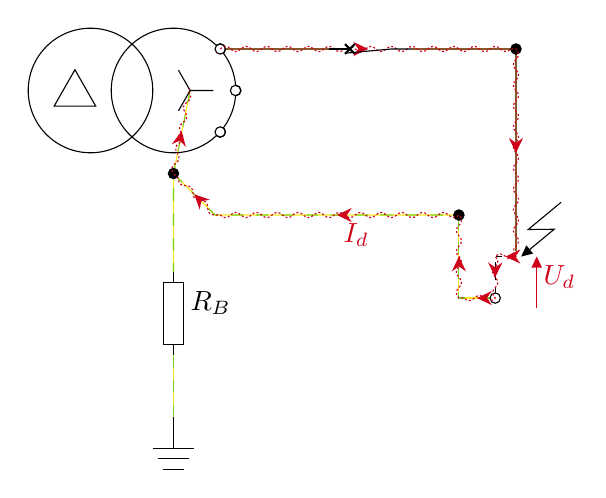
\begin{tikzpicture}[x=0.75pt,y=0.75pt,yscale=-1,xscale=1]
%uncomment if require: \path (0,251); %set diagram left start at 0, and has height of 251

%Straight Lines [id:da9415376086031365] 
\draw [color={rgb, 255:red, 0; green, 0; blue, 0 }  ,draw opacity=1 ] [dash pattern={on 2.25pt off 2.25pt}]  (242.5,132.5) -- (242.5,115) -- (252.5,115) ;
%Straight Lines [id:da5104591094158853] 
\draw [color={rgb, 255:red, 248; green, 231; blue, 28 }  ,draw opacity=1 ]   (87.5,75) -- (107.5,95) -- (225,95) ;
%Straight Lines [id:da1966201814177917] 
\draw [color={rgb, 255:red, 126; green, 211; blue, 33 }  ,draw opacity=1 ] [dash pattern={on 4.5pt off 4.5pt}]  (87.5,75) -- (107.5,95) -- (225,95) ;
%Straight Lines [id:da3955266461919331] 
\draw [color={rgb, 255:red, 248; green, 231; blue, 28 }  ,draw opacity=1 ]   (87.5,162.5) -- (87.5,192.5) ;
%Straight Lines [id:da18836033833143995] 
\draw [color={rgb, 255:red, 248; green, 231; blue, 28 }  ,draw opacity=1 ]   (240,135) -- (225,135) -- (225,95) ;
%Straight Lines [id:da17249205616306007] 
\draw [color={rgb, 255:red, 139; green, 87; blue, 42 }  ,draw opacity=1 ]   (112.5,15) -- (162.5,15) ;
%Straight Lines [id:da11309897556582038] 
\draw [color={rgb, 255:red, 248; green, 231; blue, 28 }  ,draw opacity=1 ]   (95.5,35) -- (87.5,75) -- (87.5,122.5) ;
%Straight Lines [id:da4238452834369957] 
\draw [color={rgb, 255:red, 126; green, 211; blue, 33 }  ,draw opacity=1 ] [dash pattern={on 4.5pt off 4.5pt}]  (95.5,35) -- (87.5,75) -- (87.5,122.5) ;
%Straight Lines [id:da07337279365918903] 
\draw [color={rgb, 255:red, 139; green, 87; blue, 42 }  ,draw opacity=1 ]   (202.5,15) -- (252.5,15) ;
%Shape: Path Data [id:dp3633653751506416] 
\draw   (112.5,55) .. controls (112.5,56.38) and (111.38,57.5) .. (110,57.5) .. controls (109.29,57.5) and (108.65,57.2) .. (108.19,56.72) .. controls (102.81,61.85) and (95.52,65) .. (87.5,65) .. controls (70.93,65) and (57.5,51.57) .. (57.5,35) .. controls (57.5,18.43) and (70.93,5) .. (87.5,5) .. controls (95.52,5) and (102.81,8.15) .. (108.19,13.28) .. controls (108.65,12.8) and (109.29,12.5) .. (110,12.5) .. controls (111.38,12.5) and (112.5,13.62) .. (112.5,15) .. controls (112.5,15.82) and (112.11,16.54) .. (111.5,17) .. controls (114.8,21.39) and (116.92,26.71) .. (117.4,32.5) .. controls (117.43,32.5) and (117.47,32.5) .. (117.5,32.5) .. controls (118.88,32.5) and (120,33.62) .. (120,35) .. controls (120,36.38) and (118.88,37.5) .. (117.5,37.5) .. controls (117.47,37.5) and (117.43,37.5) .. (117.4,37.5) .. controls (116.92,43.29) and (114.8,48.61) .. (111.5,53) .. controls (112.11,53.46) and (112.5,54.18) .. (112.5,55) -- cycle ;
%Shape: Circle [id:dp8103241388904666] 
\draw   (17.5,35) .. controls (17.5,18.43) and (30.93,5) .. (47.5,5) .. controls (64.07,5) and (77.5,18.43) .. (77.5,35) .. controls (77.5,51.57) and (64.07,65) .. (47.5,65) .. controls (30.93,65) and (17.5,51.57) .. (17.5,35) -- cycle ;
%Shape: Triangle [id:dp1236855376591316] 
\draw   (40,25) -- (30,42.5) -- (50,42.5) -- cycle ;
%Shape: Star [id:dp7604780706337534] 
\draw   (106.75,35) -- (95.5,35) -- (89.88,44.81) -- (95.5,35) -- (89.88,25.19) -- (95.5,35) -- cycle ;
%Shape: Circle [id:dp9987526738268633] 
\draw   (107.5,15) .. controls (107.5,13.62) and (108.62,12.5) .. (110,12.5) .. controls (111.38,12.5) and (112.5,13.62) .. (112.5,15) .. controls (112.5,16.38) and (111.38,17.5) .. (110,17.5) .. controls (108.62,17.5) and (107.5,16.38) .. (107.5,15) -- cycle ;
%Shape: Circle [id:dp06603296247595714] 
\draw   (114.9,35) .. controls (114.9,33.62) and (116.02,32.5) .. (117.4,32.5) .. controls (118.78,32.5) and (119.9,33.62) .. (119.9,35) .. controls (119.9,36.38) and (118.78,37.5) .. (117.4,37.5) .. controls (116.02,37.5) and (114.9,36.38) .. (114.9,35) -- cycle ;
%Shape: Circle [id:dp9864995024391362] 
\draw   (107.5,55) .. controls (107.5,53.62) and (108.62,52.5) .. (110,52.5) .. controls (111.38,52.5) and (112.5,53.62) .. (112.5,55) .. controls (112.5,56.38) and (111.38,57.5) .. (110,57.5) .. controls (108.62,57.5) and (107.5,56.38) .. (107.5,55) -- cycle ;

%Straight Lines [id:da23296631733343887] 
\draw [color={rgb, 255:red, 139; green, 87; blue, 42 }  ,draw opacity=1 ]   (252.5,112.5) -- (252.5,17.5) ;
%Straight Lines [id:da04537703273022686] 
\draw [color={rgb, 255:red, 126; green, 211; blue, 33 }  ,draw opacity=1 ] [dash pattern={on 4.5pt off 4.5pt}]  (240,135) -- (225,135) -- (225,95) ;
%Straight Lines [id:da014129266039552002] 
\draw    (87.5,192.5) -- (87.5,207.5) ;
%Straight Lines [id:da0064749529617041945] 
\draw    (77.5,207.5) -- (97.5,207.5) ;
%Straight Lines [id:da15495544426671526] 
\draw    (80,212.5) -- (95,212.5) ;
%Straight Lines [id:da9920646299152576] 
\draw    (82.5,217.5) -- (92.5,217.5) ;

%Straight Lines [id:da3741789060346865] 
\draw [color={rgb, 255:red, 126; green, 211; blue, 33 }  ,draw opacity=1 ] [dash pattern={on 4.5pt off 4.5pt}]  (87.5,162.5) -- (87.5,192.5) ;
%Straight Lines [id:da7734223518041439] 
\draw    (87.5,157.5) -- (87.5,162.5) ;
%Shape: Rectangle [id:dp997793865821069] 
\draw   (92.5,127.5) -- (92.5,157.5) -- (82.5,157.5) -- (82.5,127.5) -- cycle ;
%Straight Lines [id:da3149495431277475] 
\draw    (87.5,122.5) -- (87.5,127.5) ;

%Shape: Circle [id:dp16804091145958433] 
\draw  [fill={rgb, 255:red, 0; green, 0; blue, 0 }  ,fill opacity=1 ] (250,15) .. controls (250,13.62) and (251.12,12.5) .. (252.5,12.5) .. controls (253.88,12.5) and (255,13.62) .. (255,15) .. controls (255,16.38) and (253.88,17.5) .. (252.5,17.5) .. controls (251.12,17.5) and (250,16.38) .. (250,15) -- cycle ;
%Shape: Circle [id:dp448433802683451] 
\draw  [fill={rgb, 255:red, 255; green, 255; blue, 255 }  ,fill opacity=1 ] (240,135) .. controls (240,133.62) and (241.12,132.5) .. (242.5,132.5) .. controls (243.88,132.5) and (245,133.62) .. (245,135) .. controls (245,136.38) and (243.88,137.5) .. (242.5,137.5) .. controls (241.12,137.5) and (240,136.38) .. (240,135) -- cycle ;
%Shape: Circle [id:dp727181862391113] 
\draw  [fill={rgb, 255:red, 0; green, 0; blue, 0 }  ,fill opacity=1 ] (85,75) .. controls (85,73.62) and (86.12,72.5) .. (87.5,72.5) .. controls (88.88,72.5) and (90,73.62) .. (90,75) .. controls (90,76.38) and (88.88,77.5) .. (87.5,77.5) .. controls (86.12,77.5) and (85,76.38) .. (85,75) -- cycle ;
%Shape: Circle [id:dp14350658403367889] 
\draw  [fill={rgb, 255:red, 0; green, 0; blue, 0 }  ,fill opacity=1 ] (222.5,95) .. controls (222.5,93.62) and (223.62,92.5) .. (225,92.5) .. controls (226.38,92.5) and (227.5,93.62) .. (227.5,95) .. controls (227.5,96.38) and (226.38,97.5) .. (225,97.5) .. controls (223.62,97.5) and (222.5,96.38) .. (222.5,95) -- cycle ;
%Straight Lines [id:da09996473378362858] 
\draw [color={rgb, 255:red, 208; green, 2; blue, 27 }  ,draw opacity=1 ] [dash pattern={on 0.75pt off 0.75pt}]  (110,15) .. controls (111.67,13.33) and (113.33,13.33) .. (115,15) .. controls (116.67,16.67) and (118.33,16.67) .. (120,15) .. controls (121.67,13.33) and (123.33,13.33) .. (125,15) .. controls (126.67,16.67) and (128.33,16.67) .. (130,15) .. controls (131.67,13.33) and (133.33,13.33) .. (135,15) .. controls (136.67,16.67) and (138.33,16.67) .. (140,15) .. controls (141.67,13.33) and (143.33,13.33) .. (145,15) .. controls (146.67,16.67) and (148.33,16.67) .. (150,15) .. controls (151.67,13.33) and (153.33,13.33) .. (155,15) .. controls (156.67,16.67) and (158.33,16.67) .. (160,15) .. controls (161.67,13.33) and (163.33,13.33) .. (165,15) .. controls (166.67,16.67) and (168.33,16.67) .. (170,15) .. controls (171.67,13.33) and (173.33,13.33) .. (175,15) .. controls (176.67,16.67) and (178.33,16.67) .. (180,15) .. controls (181.67,13.33) and (183.33,13.33) .. (185,15) .. controls (186.67,16.67) and (188.33,16.67) .. (190,15) .. controls (191.67,13.33) and (193.33,13.33) .. (195,15) .. controls (196.67,16.67) and (198.33,16.67) .. (200,15) .. controls (201.67,13.33) and (203.33,13.33) .. (205,15) .. controls (206.67,16.67) and (208.33,16.67) .. (210,15) .. controls (211.67,13.33) and (213.33,13.33) .. (215,15) .. controls (216.67,16.67) and (218.33,16.67) .. (220,15) .. controls (221.67,13.33) and (223.33,13.33) .. (225,15) .. controls (226.67,16.67) and (228.33,16.67) .. (230,15) .. controls (231.67,13.33) and (233.33,13.33) .. (235,15) .. controls (236.67,16.67) and (238.33,16.67) .. (240,15) .. controls (241.67,13.33) and (243.33,13.33) .. (245,15) .. controls (246.67,16.67) and (248.33,16.67) .. (250,15) -- (252.5,15) -- (252.5,15) .. controls (254.17,16.67) and (254.17,18.33) .. (252.5,20) .. controls (250.83,21.67) and (250.83,23.33) .. (252.5,25) .. controls (254.17,26.67) and (254.17,28.33) .. (252.5,30) .. controls (250.83,31.67) and (250.83,33.33) .. (252.5,35) .. controls (254.17,36.67) and (254.17,38.33) .. (252.5,40) .. controls (250.83,41.67) and (250.83,43.33) .. (252.5,45) .. controls (254.17,46.67) and (254.17,48.33) .. (252.5,50) .. controls (250.83,51.67) and (250.83,53.33) .. (252.5,55) .. controls (254.17,56.67) and (254.17,58.33) .. (252.5,60) .. controls (250.83,61.67) and (250.83,63.33) .. (252.5,65) .. controls (254.17,66.67) and (254.17,68.33) .. (252.5,70) .. controls (250.83,71.67) and (250.83,73.33) .. (252.5,75) .. controls (254.17,76.67) and (254.17,78.33) .. (252.5,80) .. controls (250.83,81.67) and (250.83,83.33) .. (252.5,85) .. controls (254.17,86.67) and (254.17,88.33) .. (252.5,90) .. controls (250.83,91.67) and (250.83,93.33) .. (252.5,95) .. controls (254.17,96.67) and (254.17,98.33) .. (252.5,100) .. controls (250.83,101.67) and (250.83,103.33) .. (252.5,105) .. controls (254.17,106.67) and (254.17,108.33) .. (252.5,110) .. controls (250.83,111.67) and (250.83,113.33) .. (252.5,115) -- (252.5,115) .. controls (250.83,116.67) and (249.17,116.67) .. (247.5,115) .. controls (245.83,113.33) and (244.17,113.33) .. (242.5,115) -- (242.5,115) .. controls (244.17,116.67) and (244.17,118.33) .. (242.5,120) .. controls (240.83,121.67) and (240.83,123.33) .. (242.5,125) .. controls (244.17,126.67) and (244.17,128.33) .. (242.5,130) .. controls (240.83,131.67) and (240.83,133.33) .. (242.5,135) -- (242.5,135) -- (242.5,135) .. controls (240.83,136.67) and (239.17,136.67) .. (237.5,135) .. controls (235.83,133.33) and (234.17,133.33) .. (232.5,135) .. controls (230.83,136.67) and (229.17,136.67) .. (227.5,135) -- (225,135) -- (225,135) .. controls (223.33,133.33) and (223.33,131.67) .. (225,130) .. controls (226.67,128.33) and (226.67,126.67) .. (225,125) .. controls (223.33,123.33) and (223.33,121.67) .. (225,120) .. controls (226.67,118.33) and (226.67,116.67) .. (225,115) .. controls (223.33,113.33) and (223.33,111.67) .. (225,110) .. controls (226.67,108.33) and (226.67,106.67) .. (225,105) .. controls (223.33,103.33) and (223.33,101.67) .. (225,100) .. controls (226.67,98.33) and (226.67,96.67) .. (225,95) -- (225,95) -- (225,95) .. controls (223.33,96.67) and (221.67,96.67) .. (220,95) .. controls (218.33,93.33) and (216.67,93.33) .. (215,95) .. controls (213.33,96.67) and (211.67,96.67) .. (210,95) .. controls (208.33,93.33) and (206.67,93.33) .. (205,95) .. controls (203.33,96.67) and (201.67,96.67) .. (200,95) .. controls (198.33,93.33) and (196.67,93.33) .. (195,95) .. controls (193.33,96.67) and (191.67,96.67) .. (190,95) .. controls (188.33,93.33) and (186.67,93.33) .. (185,95) .. controls (183.33,96.67) and (181.67,96.67) .. (180,95) .. controls (178.33,93.33) and (176.67,93.33) .. (175,95) .. controls (173.33,96.67) and (171.67,96.67) .. (170,95) .. controls (168.33,93.33) and (166.67,93.33) .. (165,95) .. controls (163.33,96.67) and (161.67,96.67) .. (160,95) .. controls (158.33,93.33) and (156.67,93.33) .. (155,95) .. controls (153.33,96.67) and (151.67,96.67) .. (150,95) .. controls (148.33,93.33) and (146.67,93.33) .. (145,95) .. controls (143.33,96.67) and (141.67,96.67) .. (140,95) .. controls (138.33,93.33) and (136.67,93.33) .. (135,95) .. controls (133.33,96.67) and (131.67,96.67) .. (130,95) .. controls (128.33,93.33) and (126.67,93.33) .. (125,95) .. controls (123.33,96.67) and (121.67,96.67) .. (120,95) .. controls (118.33,93.33) and (116.67,93.33) .. (115,95) .. controls (113.33,96.67) and (111.67,96.67) .. (110,95) -- (107.5,95) -- (107.5,95) .. controls (105.14,95) and (103.96,93.82) .. (103.96,91.46) .. controls (103.96,89.11) and (102.78,87.93) .. (100.43,87.93) .. controls (98.07,87.93) and (96.89,86.75) .. (96.89,84.39) .. controls (96.89,82.04) and (95.71,80.86) .. (93.36,80.86) .. controls (91,80.86) and (89.82,79.68) .. (89.82,77.32) -- (87.5,75) -- (87.5,75) .. controls (86.17,73.05) and (86.48,71.42) .. (88.43,70.09) .. controls (90.38,68.76) and (90.69,67.12) .. (89.36,65.17) .. controls (88.03,63.22) and (88.34,61.59) .. (90.29,60.26) .. controls (92.24,58.93) and (92.54,57.3) .. (91.21,55.35) .. controls (89.88,53.4) and (90.19,51.77) .. (92.14,50.44) .. controls (94.09,49.11) and (94.4,47.47) .. (93.07,45.52) .. controls (91.74,43.57) and (92.05,41.94) .. (94,40.61) .. controls (95.95,39.28) and (96.26,37.65) .. (94.93,35.7) -- (95.25,34) -- (95.25,34) ;
\draw [shift={(181.25,15)}, rotate = 180] [fill={rgb, 255:red, 208; green, 2; blue, 27 }  ,fill opacity=1 ][line width=0.08]  [draw opacity=0] (7.14,-3.43) -- (0,0) -- (7.14,3.43) -- (4.74,0) -- cycle    ;
\draw [shift={(252.5,65)}, rotate = 270] [fill={rgb, 255:red, 208; green, 2; blue, 27 }  ,fill opacity=1 ][line width=0.08]  [draw opacity=0] (7.14,-3.43) -- (0,0) -- (7.14,3.43) -- (4.74,0) -- cycle    ;
\draw [shift={(247.5,115)}, rotate = 360] [fill={rgb, 255:red, 208; green, 2; blue, 27 }  ,fill opacity=1 ][line width=0.08]  [draw opacity=0] (7.14,-3.43) -- (0,0) -- (7.14,3.43) -- (4.74,0) -- cycle    ;
\draw [shift={(242.5,125)}, rotate = 270] [fill={rgb, 255:red, 208; green, 2; blue, 27 }  ,fill opacity=1 ][line width=0.08]  [draw opacity=0] (7.14,-3.43) -- (0,0) -- (7.14,3.43) -- (4.74,0) -- cycle    ;
\draw [shift={(233.75,135)}, rotate = 360] [fill={rgb, 255:red, 208; green, 2; blue, 27 }  ,fill opacity=1 ][line width=0.08]  [draw opacity=0] (7.14,-3.43) -- (0,0) -- (7.14,3.43) -- (4.74,0) -- cycle    ;
\draw [shift={(225,115)}, rotate = 450] [fill={rgb, 255:red, 208; green, 2; blue, 27 }  ,fill opacity=1 ][line width=0.08]  [draw opacity=0] (7.14,-3.43) -- (0,0) -- (7.14,3.43) -- (4.74,0) -- cycle    ;
\draw [shift={(166.25,95)}, rotate = 360] [fill={rgb, 255:red, 208; green, 2; blue, 27 }  ,fill opacity=1 ][line width=0.08]  [draw opacity=0] (7.14,-3.43) -- (0,0) -- (7.14,3.43) -- (4.74,0) -- cycle    ;
\draw [shift={(97.5,85)}, rotate = 405] [fill={rgb, 255:red, 208; green, 2; blue, 27 }  ,fill opacity=1 ][line width=0.08]  [draw opacity=0] (7.14,-3.43) -- (0,0) -- (7.14,3.43) -- (4.74,0) -- cycle    ;
\draw [shift={(91.38,54.5)}, rotate = 460.7] [fill={rgb, 255:red, 208; green, 2; blue, 27 }  ,fill opacity=1 ][line width=0.08]  [draw opacity=0] (7.14,-3.43) -- (0,0) -- (7.14,3.43) -- (4.74,0) -- cycle    ;
%Shape: Boxed Line [id:dp3673372749832414] 
\draw    (274.27,88.83) -- (258.39,101.97) -- (270.89,101.86) -- (257.31,113.09) ;
\draw [shift={(255,115)}, rotate = 320.40999999999997] [fill={rgb, 255:red, 0; green, 0; blue, 0 }  ][line width=0.08]  [draw opacity=0] (5.36,-2.57) -- (0,0) -- (5.36,2.57) -- cycle    ;
%Straight Lines [id:da5575509867036751] 
\draw    (170.5,17) -- (192.5,15) -- (202.5,15) ;
%Straight Lines [id:da508912305096757] 
\draw    (172.5,15) -- (162.5,15) ;
\draw [shift={(172.5,15)}, rotate = 225] [color={rgb, 255:red, 0; green, 0; blue, 0 }  ][line width=0.75]    (-3.35,0) -- (3.35,0)(0,3.35) -- (0,-3.35)   ;

%Straight Lines [id:da16958097231268054] 
\draw [color={rgb, 255:red, 208; green, 2; blue, 27 }  ,draw opacity=1 ]   (262.5,118) -- (262.5,140) ;
\draw [shift={(262.5,115)}, rotate = 90] [fill={rgb, 255:red, 208; green, 2; blue, 27 }  ,fill opacity=1 ][line width=0.08]  [draw opacity=0] (5.36,-2.57) -- (0,0) -- (5.36,2.57) -- cycle    ;


% Text Node
\draw (94.5,130.5) node [anchor=north west][inner sep=0.75pt]   [align=left] {$R_B$};
% Text Node
\draw (168.25,98) node [anchor=north west][inner sep=0.75pt]  [color={rgb, 255:red, 208; green, 2; blue, 27 }  ,opacity=1 ] [align=left] {$I_d$};
% Text Node
\draw (264.5,118) node [anchor=north west][inner sep=0.75pt]  [color={rgb, 255:red, 208; green, 2; blue, 27 }  ,opacity=1 ] [align=left] {$U_d$};


\end{tikzpicture}

\end{figure}

%\end{document}



Pour calculer le courant de défaut $I_d$, il existe trois méthode, mais ne sera détaillé dans ce chapitre que la première (plus de précisions sur les deux autres méthode \superref{ann:schema_tn}) :
\begin{itemize}
\item Méthode conventionnelle\,;
\item Méthode des impédances\,;
\item Méthode de composition.
\end{itemize}

\section{Méthode de dimensionnement conventionnelle des protections et des sections de conducteurs\label{sec:schema_tn_methode_conventionnelle}}

Contrairement au SLT TT, il ne faut pas tenir compte de la \emph{résistance de défaut} $R_d$ qui prend en compte la nature du défaut d'isolement (franc ou non-franc) et la résistance de la carcasse métallique car il s'agit d'un court-circuit et elle sera donc très faible.\\
$I_d$ s'apparente donc à un courant de court-circuit et son calcul est basé sur l'hypothèse que la tension de défaut reste supérieur à 80\% ou plus de la tension nominale simple. Cette valeur est issue d'une estimation de la chute de tension due à l'ensemble des impédances en amont de la protection du circuit en défaut. Elle est utilisée, avec l'impédance de la boucle de circuit, pour calculer ce courant de court-circuit.\\ 

Ce facteur est calculé par l'estimation de la chute de tension due à l'ensemble des impédances en amont de cette origine. Dans une majorité des types de pose, les réactances inductive interne et entres les conducteurs sont négligées, ce qui revient à ne considérer que les résistances des conducteurs dans les calculs d'intensité de court-circuit. Cette approximation est considérée comme valable pour les sections de câble jusqu'à \SI{120}{\square\milli\meter}. Au-dessus de cette section, la résistance $R$ des conducteurs est augmentée selon le tableau ci-dessous :

\begin{table}[H]
\caption{Section des conducteurs (schéma TN / méthode conventionnelle)}
\begin{tabularx}{0.8\linewidth}{Q K@{${\enspace{}}+{\enspace{}}$}I}
\toprule
\multicolumn{2}{c}{\thead{Section des conducteurs}} & \multicolumn{2}{c}{\thead{Ajustement de la résistance en \si{\ohm}}} \\
\midrule
S & \SI{150}{\square\milli\meter} & R & 15\% \\
S & \SI{185}{\square\milli\meter} & R & 20\% \\
S & \SI{240}{\square\milli\meter} & R & 25\% \\
\bottomrule
\end{tabularx}
\end{table}

\begin{formule}{Courant de défaut $I_d$ en schéma TN selon la méthode conventionnelle}{courant_defaut_tn_conventionnel}
\begin{align*}
		I_d &= \frac{0,8 \times U_{0}}{R_{PE}+R_{ph}} \\
		I_d &= \frac{0,8 \times U_{0}}{Z_{c}}
\end{align*}

\begin{textvariables}
U_{0}						& tension							& volt			& \volt					& 	Tension nominale simple \\
0,8							& facteur							& 					& 	/						& 	facteur d'approximation de la tension de défaut $U_d$ \\
R_{PE}						& résistance						& ohm			& \ohm					& 	Résistance du conducteur de phase traversé par un courant de défaut $I_d$	\\
R_{ph}						& résistance						& ohm			& \ohm					& 	Résistance du conducteur PE traversé par un courant de défaut $I_d$ \\
Z_{c}						& impédance						& ohm			& \ohm					& Impédance de boucle du circuit en défaut (selon la méthode conventionnelle)\\
\end{textvariables}
\end{formule}

Le courant de défaut $I_d$ fera alors apparaître une \emph{tension de défaut} $U_d$ entre la masse métallique et la terre :

\begin{formule}{Tension de défaut $U_d$ en schéma TN selon la méthode conventionnelle}{}
\begin{align*}
		U_d &= R_{PE} \times I_{d}
\end{align*}

\begin{textvariables}
R_{PE}						& résistance						& ohm			& \ohm					& 	Résistance du conducteur PE traversé par un courant de défaut $I_d$	\\
I_{d}							& intensité							& ampère		& \ampere				& 	Courant de défaut d'isolement \\
\end{textvariables}
\end{formule}

La tension de défaut $U_d$ dans le cas d'un défaut d'isolement en régime TN est \emph{élevée} et donc \emph{dangereuse} si elle est supportée trop longtemps. La norme NF C15-100 a défini des temps de coupure maximum à respecter :

%--------------------------------------
%ELECTROTECHNIQUE - SCHEMA DE LIAISON A LA TERRE
%--------------------------------------

%utiliser les environnement \begin{comment} \end{comment} pour mettre en commentaire le préambule une fois la programmation appelée dans le document maître (!ne pas oublier de mettre en commentaire \end{document}!)

\begin{comment}

\documentclass[a4paper, 11pt, twoside, fleqn]{memoir}

\usepackage{AOCDTF}

\marqueurchapitre
\decoupagechapitre{1} %juste pour éviter les erreurs lors de la compilation des sous-programmations (passera en commentaire)

%lien d'édition des figures Tikz sur le site mathcha.io (rajouter le lien d'une modification effectuée sur la figure tikz avec le nom du modificateur car il n'y a qu'un lien par compte)

%lien éditeur Bruno Douchy : https://www.mathcha.io/editor/zjygnFElSdyhJ72e3zT5ZgqwBT4DKnovswpXn1q

%--------------------------------------
%corps du document
%--------------------------------------

\begin{document} %corps du document
	\openleft %début de chapitre à gauche

\end{comment}

\begin{table}[H]
\caption{Temps de coupure maximal des disjoncteurs en schéma TN\label{tab:schema_tn_temps_coupure}}
\begin{tabularx}{\textwidth}{C C C}
\toprule
\multirow[c]{2}{*}{\thead{Réseaux usuels}} & \multicolumn{2}{c}{\thead{Temps de coupure maximal en \si{\milli\second}}}\\
\cmidrule(lr){2-3} 
	& $U_{L}=\SI{50}{\volt}$ 	& 			$U_{L}=\SI{25}{\volt}$  \\
\midrule
\SI{127}{\volt}/\SI{230}{\volt}		& 800		& 350 \\
\SI{230}{\volt}/\SI{400}{\volt}		& 400		& 200 \\
\SI{400}{\volt}/\SI{690}{\volt}		& 200		& 50 \\
\SI{690}{\volt}/\SI{1000}{\volt}	& 100		& 20 \\
\bottomrule 
\end{tabularx}
\end{table}

%\end{document}



\begin{formule}{Seuil de réglage du disjoncteur $I_m$ en schéma TN}{}
\begin{align*}
		I_{m} &> I_{d}
\end{align*}

\begin{textvariables}
I_{m}						& intensité							& ampère			& \ampere					& 	Intensité de seuil de déclenchement de la protection magnétique du disjoncteur \\
\end{textvariables}
\end{formule}

On peut calculer la longueur maximale d'un circuit d'une installation en schéma TN par la formule suivante :\\

\begin{formule}{Longueur maximale d'un circuit $L_{max}$}{schema_tn_longueur_max_circuit}
\begin{align*}
		L_{max} &= \frac{0,8 \times U_{0} \times S_{ph}}{\rho \times (1+m) \times I_m}\\
		m &= \frac{S_{ph}}{S_{PE}}
\end{align*}
\begin{textvariables}
I_{m}						& intensité							& ampère			& \ampere							& 	Intensité de seuil de déclenchement de la protection magnétique du disjoncteur \\
U_{0}						& tension							& volt				& \volt								& 	Tension nominale simple \\
S_{ph}						& section							& millimètre\up{2}		& \si{\square\milli\meter}	& 	Section du conducteur de phase traversé par un courant de défaut $I_d$ \\
S_{PE}						& section							& millimètre\up{2}		& \si{\square\milli\meter}	& 	Section du conducteur PE traversé par un courant de défaut $I_d$ \\
\rho							& résistivité						& 									& /	& 	Résistivité du conducteur (selon la température et le matériau choisi) :
\begin{tabdescription}
\item[aluminium :] \SI{37.6e-3}{\ohm\square\milli\meter\per\meter}
\item[cuivre :] \SI{22.5e-3}{\ohm\square\milli\meter\per\meter}
\end{tabdescription}\\
m								& facteur		& 			& /										& Facteur de correction à appliquer aux valeurs données dans les abaques de détermination des longueurs selon la section et l'intensité de déclenchement (\superref{subsubsec:facteur_correction_m}) 	 \\
\end{textvariables}
\end{formule}


Pour vérifier rapidement un dimensionnement, les constructeurs de protections ont établis des abaques permettant de déterminer rapidement les longueurs maximale des conducteurs selon l'intensité, la section des conducteurs ou en encore les réglages du seuil de courant de déclenchement du disjoncteur ou encore le type de disjoncteurs. Ces abaques sont issus des norme IEC 60947-2\supercite{IEC:60947-2-2016} et IEC 60898\supercite{IEC:60898-2015}, qui concernent respectivement les disjoncteurs industriels et domestiques. Ils sont détaillés dans l'annexe \superref{ann:schema_tn}.

\begin{exemple}{Calcul du courant de défaut $I_d$ en schéma TN selon la méthode conventionnelle}{}
Si on considère que les conducteurs sont en cuivre, que $U_{0}=\SI{230}{\volt}$, que $L_{ph}=\SI{50}{\meter}$ et est équivalent à $L_{PE}$, que $S_{ph}=\SI{35}{\square\milli\meter}$ et est équivalent à  $S_{PE}$, on peut déduire que le courant de défaut $I_d$ vaut :
\begin{align*}
		Z_{c}	&= 2 \times \rho \times \frac{L}{S}  								& 			I_d		&= \frac{U_0 \times 0,8}{Z_c} \\
					&= 2 \times 22.5 \times 10^{-3} \times \frac{50}{35} 	&						&= \frac{230 \times 0,8}{64,3 \times 10^{-3}} \\
					&= \SI{64,3}{\milli\ohm}						 						& 						&= \SI{2816}{\ampere}
\end{align*}
\end{exemple}

\begin{exemple}{Calcul de la longueur maximale des conducteurs $L_{max}$ en schéma TN selon la méthode conventionnelle}{}
Si on considère que les conducteurs sont en cuivre, que $U_{0}=\SI{230}{\volt}$, que $L{ph}=\SI{50}{\meter}$ et est équivalent à $L{PE}$, que $S_{ph}=\SI{35}{\square\milli\meter}$ et est équivalent à  $S_{PE}$, on peut déduire que le courant de défaut $I_d$ vaut :
\begin{align*}
		Z_{c}	&= 2 \times \rho \times \frac{L}{S}  								& 			I_d		&= \frac{U_0 \times 0,8}{Z_c} \\
					&= 2 \times 22.5 \times 10^{-3} \times \frac{50}{35} 			&				&= \frac{230 \times 0,8}{64,3e \times 10^{-3}} \\
					&= \SI{64,3}{\milli\ohm}						 						& 						&= \SI{2816}{\ampere}
\end{align*}

Il convient de croiser cette valeur de $I_d$ avec les valeurs du seuil de déclenchement du disjoncteur Instantané et Court-retard et leurs temps de coupures respectifs (voir \superref{tab:schema_tn_temps_coupure}) pour valider le dimensionnement et le choix de la protection.
\end{exemple}

\section{Protection avec des DDR en schéma TN}

La protection des circuits à l'aide de DDR en schéma TN est formellement interdite en schéma TN-C car le conducteur PE ne peut pas être sectionné. En schéma TN-C-S, son utilisation implique forcément que les conducteurs PE et N soient séparés en amont du DDR.\\

Les DDR en schéma TN-S sont requis lorsque :
\begin{itemize}
\item l'impédance de la boucle de défaut $Z_c$ n'est pas précisément calculable\,;
\item le courant de défaut est trop faible pour que la protection détecte le défaut comme s'apparentant à un court-circuit dans le temps de déconnexion requis.
\end{itemize}

Un DDR se déclenchant avec un courant de déclenchement de l'ordre que quelques ampères maximum, il convient bien à un circuit terminal d'une installation BT conséquente en schéma TN.

\end{document}
